\documentclass[11pt,a4paper,openany]{book}
\usepackage[T1]{fontenc}
\usepackage[utf8]{inputenc}
\usepackage[sc]{mathpazo}
\linespread{1.06}
\usepackage[scaled=0.9]{helvet}
\renewcommand{\ttdefault}{lmtt}
\usepackage{amsmath,amssymb,amsthm}
\usepackage{microtype}
\usepackage[a4paper,top=2.6cm,bottom=2.8cm,inner=2.8cm,outer=2.8cm]{geometry}
\usepackage[dvipsnames]{xcolor}
\usepackage{graphicx}
\usepackage{caption}
\usepackage{booktabs,tabularx}
\newcolumntype{Y}{>{\raggedright\arraybackslash}X}
\renewcommand{\arraystretch}{1.2}
\usepackage{enumitem}
\usepackage{alltt}
\usepackage[most]{tcolorbox}
\usepackage{titlesec}
\usepackage{fancyhdr}
\usepackage[hidelinks,bookmarksnumbered]{hyperref}
\hypersetup{colorlinks=true,linkcolor=thmc,urlcolor=thmc,citecolor=thmc,
  pdftitle={Regret and Rebalancing},pdfsubject={Online learning with applications to finance}}

% ---- palette (matches the HTML edition, light theme) ----
\definecolor{ink}{HTML}{1A1F24}
\definecolor{muted}{HTML}{58616B}
\definecolor{rulec}{HTML}{D5D9CF}
\definecolor{thmc}{HTML}{1E4E79}\definecolor{thmsoft}{HTML}{E3EAF1}
\definecolor{defc}{HTML}{2F6B4F}\definecolor{defsoft}{HTML}{E5EFE8}
\definecolor{finc}{HTML}{8A5A12}\definecolor{finsoft}{HTML}{F4ECDD}
\definecolor{warnc}{HTML}{9A3B26}\definecolor{warnsoft}{HTML}{F5E6E1}
\definecolor{codebg}{HTML}{EEF0EA}
\definecolor{panel}{HTML}{EAECE5}

% ---- macros used in the math (same as the MathJax config) ----
\newcommand{\R}{\mathbb{R}}
\newcommand{\E}{\mathbb{E}}
\newcommand{\eps}{\varepsilon}
\newcommand{\Reg}{\mathrm{Regret}}
\newcommand{\ind}{\mathbf{1}}
\newcommand{\KL}{\mathrm{KL}}
\DeclareMathOperator*{\argmin}{arg\,min}
\DeclareMathOperator*{\argmax}{arg\,max}
\newcommand{\ip}[2]{\langle #1,#2\rangle}
\newcommand{\norm}[1]{\lVert #1\rVert}
\newcommand{\abs}[1]{\lvert #1\rvert}
\newcommand{\simplex}{\Delta}
\newcommand{\hy}{\hat{y}}
\newcommand{\cK}{\mathcal{K}}
\newcommand{\cS}{\mathcal{S}}

% ---- headings ----
\titleformat{\chapter}[display]{\sffamily\bfseries\color{ink}}
  {\normalsize\color{thmc}\MakeUppercase{\chaptertitlename}\ \thechapter}{4pt}{\huge}
\titlespacing*{\chapter}{0pt}{0pt}{18pt}
\titleformat{\section}{\sffamily\bfseries\Large\color{ink}}{\thesection}{0.8em}{}
\titleformat{\subsection}{\sffamily\bfseries\large\color{ink}}{\thesubsection}{0.8em}{}
\newcommand{\thepartblurb}{}
\titleformat{\part}[display]{\centering\sffamily\bfseries\color{thmc}}{\Large\partname\ \thepart}{12pt}{\Huge}
  [\partblurbbox]
\newcommand{\partblurbbox}{\vspace{2em}{\normalfont\rmfamily\mdseries\itshape\large\color{ink}\begin{minipage}{0.7\linewidth}\centering\thepartblurb\end{minipage}\par}}
\newcommand{\chapsource}[1]{{\small\sffamily\color{muted}#1\par}\medskip}
\pagestyle{fancy}
\fancyhf{}
\fancyhead[LE,RO]{\small\sffamily\thepage}
\fancyhead[RE]{\small\sffamily\color{muted}\leftmark}
\fancyhead[LO]{\small\sffamily\color{muted}\rightmark}
\renewcommand{\headrulewidth}{0pt}
\renewcommand{\chaptermark}[1]{\markboth{#1}{#1}}
\setcounter{tocdepth}{1}
\setlength{\emergencystretch}{3em}
\setlength{\parskip}{0.35em}
\setlist{itemsep=2pt,topsep=4pt}

% ---- boxes ----
\tcbset{bookbox/.style={enhanced,breakable,boxrule=0pt,leftrule=3pt,arc=2pt,
  left=8pt,right=8pt,top=6pt,bottom=6pt,before skip=10pt,after skip=10pt,
  fonttitle=\sffamily\bfseries\small,coltitle=#1,colbacktitle=white!0,
  attach title to upper,after title={\par\smallskip}}}
\newtcolorbox{bthm}[1]{bookbox=thmc,colback=thmsoft,colframe=thmc,title={#1}}
\newtcolorbox{bdef}[1]{bookbox=defc,colback=defsoft,colframe=defc,title={#1}}
\newtcolorbox{bfin}[1]{bookbox=finc,colback=finsoft,colframe=finc,title={#1}}
\newtcolorbox{bwarn}[1]{bookbox=warnc,colback=warnsoft,colframe=warnc,title={#1}}
\newtcolorbox{balg}[1]{bookbox=ink,colback=panel,colframe=muted,title={#1}}
\newtcolorbox{bexample}[1]{bookbox=muted,colback=white,colframe=muted,title={#1}}
\newtcolorbox{goals}{enhanced,breakable,boxrule=0.4pt,arc=2pt,colback=white,colframe=rulec,
  fonttitle=\sffamily\bfseries\small,coltitle=thmc,title={In this chapter},attach title to upper,after title={\par}}
\newtcolorbox{takeaways}{enhanced,breakable,boxrule=0pt,arc=2pt,colback=panel,
  fonttitle=\sffamily\bfseries\small,coltitle=ink,title={Key takeaways},attach title to upper,after title={\par}}
\newenvironment{marginnote}{\par\medskip\noindent\color{muted}\small\sffamily\rule{\linewidth}{0.4pt}\par}{\par\medskip}
\newenvironment{algo}{\par\smallskip\begingroup\footnotesize\begin{alltt}}{\end{alltt}\endgroup\smallskip}

% ---- exercises ----
\newcommand{\extag}[2]{%
  \def\tmp{#1}\def\tmpE{easy}\def\tmpM{med}\def\tmpH{hard}%
  \ifx\tmp\tmpE\def\tagc{defc}\else\ifx\tmp\tmpM\def\tagc{thmc}\else\ifx\tmp\tmpH\def\tagc{warnc}\else\def\tagc{finc}\fi\fi\fi
  \tcbox[on line,boxrule=0pt,arc=2pt,colback=\tagc!12,left=2pt,right=2pt,top=0pt,bottom=0pt,boxsep=1pt]{\sffamily\scriptsize\bfseries\color{\tagc}#2}}
\newcommand{\exercise}[3]{\par\medskip\noindent\textbf{\sffamily #1}\ \ #2\ \ #3\par}
\newenvironment{solutions}{\small}{}
\newcommand{\sol}[2]{\par\smallskip\noindent\textbf{\sffamily #1.}\ #2\par}

\begin{document}
\frontmatter
\begin{titlepage}
\centering
\vspace*{2cm}
{\small\color{muted}\sffamily A self-study textbook · after EECS 598 “Prediction, Learning, and Games”, University of Michigan, Fall 2013\par}
\vspace{2.2cm}
{\fontsize{34}{40}\selectfont\bfseries\color{thmc} Regret and Rebalancing\par}
\vspace{1cm}
\begin{minipage}{0.8\linewidth}\centering\large Online learning from first principles, with applications to portfolios, option pricing and trading. Eighteen chapters, worked proofs, finance sidebars, and exercises with solutions.\end{minipage}
\vspace{1.6cm}
{\large\[\underbrace{\sum_{t=1}^{T}\ell_t(x_t)}_{\text{what you paid}}\;-\;\underbrace{\min_{x\in\mathcal K}\sum_{t=1}^{T}\ell_t(x)}_{\text{best fixed choice in hindsight}}\;=\;o(T)\quad\text{on every sequence.}\]}
\vfill
{\small\sffamily\noindent \begin{minipage}[t]{0.3\linewidth}\raggedright\textbf{Source course}\\ Jacob Abernethy, EECS 598-006, 24 lectures\end{minipage}\hfill\begin{minipage}[t]{0.3\linewidth}\raggedright\textbf{Companion texts}\\ Cesa-Bianchi \& Lugosi (2006); Shafer \& Vovk (2001)\end{minipage}\hfill\begin{minipage}[t]{0.3\linewidth}\raggedright\textbf{Prerequisites}\\ Probability, calculus, basic convex analysis\end{minipage}\par}
\vspace{1cm}
{\small\color{muted} Online edition with interactive demos: \texttt{regret-and-rebalancing.html}\par}
\end{titlepage}

\tableofcontents
\chapter*{How to use this book}\addcontentsline{toc}{chapter}{How to use this book}

Each chapter follows one or more lectures from the course and links to the original scribe notes. Chapters open with what you will learn and close with key takeaways and exercises; solutions are folded under each exercise so you can try first. Boxes are colour-coded: \textcolor{thmc}{\textbf{blue}} for theorems and lemmas, \textcolor{defc}{\textbf{green}} for definitions and protocols, \textcolor{finc}{\textbf{amber}} for finance applications, \textcolor{warnc}{\textbf{red}} for warnings and pitfalls. Exercise tags mark difficulty: \extag{easy}{warm-up} \extag{med}{core} \extag{hard}{challenge} \extag{fin}{finance}.

\textbf{Suggested paths.} For the core theory, read Chapters 1–3, 5, 6, 9 and 10. For finance, add Chapters 4, 11 and 12, then 13–14 for trading decisions under partial feedback, and finish with Part VII (Chapters 17–18), which takes the theory to the trading desk. Part VI (Chapters 15–16) ties the theory together and is the most abstract.

\mainmatter

\def\thepartblurb{How to learn from a crowd of forecasters when nobody promises the future looks like the past.}\part{Prediction with Expert Advice}\label{part1}

\chapter[The online learning game]{The Online Learning Game}\label{ch1}
\chapsource{Based on Lecture 1 (Sept 4, 2013) · \href{https://web.eecs.umich.edu/~jabernet/eecs598course/fall2013/web/notes/lec1_090413.pdf}{scribe notes}}

\begin{goals}
\begin{itemize}
\item The protocol of sequential prediction, and why we analyse it against an adversary.
\item Regret: the yardstick that makes adversarial analysis meaningful.
\item The Halving algorithm and its $\log_2 N$ mistake bound.
\end{itemize}
\end{goals}

\section*{1.1 Why study learning as a game?}\addcontentsline{toc}{section}{1.1 Why study learning as a game?}\label{ch1-why}

Classical statistics assumes data are drawn i.i.d. from a fixed distribution, then asks how well a model fitted on the past generalises to the future. Financial markets, spam filters, ad auctions and opponents in a game all violate that assumption: the data react to you, drift over time, or are chosen by someone with their own objective.

Online learning drops the probabilistic assumption entirely. Data arrive one at a time; after each, the learner must commit to a decision, then sees the outcome and pays a loss. The outcomes can be arbitrary, even chosen by an adversary who knows our algorithm. It sounds hopeless to promise anything in this setting, and yet the central discovery of the field (Hannan, 1957; Blackwell, 1956; Littlestone and Warmuth, 1989) is that we can guarantee to perform nearly as well as the best of a fixed set of strategies, \emph{in hindsight}, on every sequence.

\begin{center}\small
\begin{tabularx}{\linewidth}{lYY}
\toprule
\textbf{Year} & \textbf{Who} & \textbf{Idea} \\
\midrule
1956 & Blackwell & Approachability: a vector-valued minimax theorem \\
1957 & Hannan & Sequential decisions with vanishing regret, no stochastic assumptions \\
1957 & Rosenblatt & The Perceptron \\
1989–94 & Littlestone, Warmuth; Vovk & Weighted Majority; aggregating algorithms \\
1991 & Cover & Universal portfolios \\
1997 & Freund, Schapire & Hedge and AdaBoost \\
2003 & Zinkevich & Online convex optimization \\
2005 & Kalai, Vempala & Follow the Perturbed Leader \\
\bottomrule
\end{tabularx}
\end{center}

The same machinery turns up across this book: computing equilibria of zero-sum games (Chapter 6), boosting weak classifiers (Chapter 7), stochastic gradient descent (Chapter 9), portfolio selection and option pricing (Chapters 11 and 12), bandits (Chapters 13 and 14), and calibrated forecasting (Chapter 16).

\section*{1.2 Prediction with expert advice}\addcontentsline{toc}{section}{1.2 Prediction with expert advice}\label{ch1-protocol}

The simplest version: every morning $N$ pundits predict whether the market will close up ($1$) or down ($0$). We want to aggregate them.

\begin{bdef}{Protocol 1.1 \emph{(binary prediction with experts)}}
For rounds $t = 1, 2, \dots, T$:

\begin{enumerate}
\item Each expert $i\in[N]$ announces advice $f_{i,t}\in\{0,1\}$.
\item The learner (the ``master algorithm'', MA) predicts $\hy_t\in\{0,1\}$.
\item Nature reveals the outcome $y_t\in\{0,1\}$.
\end{enumerate}

The learner's performance is its number of mistakes, $M_T(\mathrm{MA}) = \sum_{t=1}^T \ind[\hy_t\neq y_t]$. Expert $i$'s mistakes $M_T(i)$ are defined the same way.
\end{bdef}

Nature is allowed to be adversarial: $y_t$ may depend on everything that happened before, including the learner's algorithm. We therefore cannot hope to bound $M_T(\mathrm{MA})$ in absolute terms. An adversary can make any deterministic learner wrong on every round by setting $y_t = 1-\hy_t$. What we can do is compare to the experts.

\begin{bdef}{Definition 1.2 \emph{(regret)}}
Given losses $\ell_t(\cdot)$, the regret of the learner with respect to a class of comparators $\mathcal{C}$ is

\[\Reg_T \;=\; \sum_{t=1}^T \ell_t(\text{learner}) \;-\; \min_{c\in\mathcal C}\sum_{t=1}^T \ell_t(c).\]

An algorithm is \textbf{no-regret} (or Hannan consistent) if $\Reg_T = o(T)$ for every sequence, so that its average loss per round is asymptotically no worse than that of the best comparator in hindsight.
\end{bdef}

Regret is the idea that makes the adversarial setting workable. If every expert is terrible, the adversary has made the problem hard and we are not blamed. If some expert is good, we must eventually do nearly as well as it, without knowing in advance which one it is.

\section*{1.3 The realizable case: Halving}\addcontentsline{toc}{section}{1.3 The realizable case: Halving}\label{ch1-halving}

Start with a strong assumption: one expert is perfect, $M_T(i^*) = 0$. Then any expert that errs even once can be discarded forever.

\begin{balg}{Algorithm 1.3 \emph{(Halving)}}
\begin{algo}
C\_1 \ensuremath{\leftarrow} \{1, …, N\}                       \# experts consistent so far
for t = 1, …, T:
    receive advice f\_\{i,t\} for i \ensuremath{\in} C\_t
    predict \ensuremath{\hat{y}}\_t \ensuremath{\leftarrow} majority vote of C\_t    (ties \ensuremath{\to} 1)
    observe y\_t
    C\_\{t+1\} \ensuremath{\leftarrow} \{ i \ensuremath{\in} C\_t : f\_\{i,t\} = y\_t \}
\end{algo}
\end{balg}

\begin{bthm}{Theorem 1.4 \emph{(Halving mistake bound)}}
If at least one expert is perfect, Halving makes at most $\log_2 N$ mistakes, on any sequence.
\end{bthm}

\begin{proof}
We track the size of the version space $C_t$. Initially $\abs{C_1}=N$. The perfect expert is never removed, so $\abs{C_t}\ge1$ for all $t$. Whenever Halving errs, at least half of $C_t$ predicted wrongly and is removed, so $\abs{C_{t+1}}\le\tfrac12\abs{C_t}$. On other rounds $C$ can only shrink. After $M$ mistakes,

\[1\;\le\;\abs{C_{T+1}}\;\le\;N\,2^{-M},\]

so $2^M\le N$, i.e. $M\le\log_2 N$.
\end{proof}

\textbf{Tightness.} Take $N=2^n$ experts indexed by binary strings, with expert $i$ predicting bit $t$ of $i$ on round $t\le n$. Each round the survivors split evenly, and the adversary picks the outcome opposite to Halving's prediction. Halving errs on each of the first $n=\log_2N$ rounds, and exactly one expert (the one matching the adversary's choices) is perfect. No deterministic algorithm can do better on this family, so $\log_2 N$ is optimal.

The proof uses a pattern that recurs throughout the book. We choose a \emph{potential} (here $\abs{C_t}$) that is bounded below because of a good comparator, and that drops by a constant factor whenever the learner suffers. The learner's loss is then bounded by how far the potential can fall.

\begin{bexample}{Example 1.5 \emph{(predictive sorting)}}
$K$ teams have an unknown true ranking $\pi^*\in S_K$. Each round two teams $(i_t,j_t)$ play and we predict the winner; the better-ranked team always wins. Treat each of the $K!$ permutations as an expert. Halving guarantees at most $\log_2 K! = O(K\log K)$ mistakes, the same count as comparisons needed to sort.

The catch is computation. Halving must compare the number of permutations consistent with the observed games that rank $i_t$ above $j_t$ against those that rank it below. That count is the number of linear extensions of a partial order, which is \#P-hard to compute (Brightwell and Winkler, 1991). The course posed as a challenge whether a polynomial-time algorithm can achieve the same mistake bound. It is a first example of a tension that runs through the field: the statistically optimal aggregation over an exponentially large expert class may be computationally intractable, unless the class has structure we can exploit (see Exercise 1.4 and Chapter 4).
\end{bexample}

\begin{bfin}{In finance}
Think of the experts as trading signals: a momentum rule, a mean-reversion rule, an analyst's recommendation, and so on. The assumption that one signal is perfect is absurd for markets, which is why Halving is only a warm-up. The regret framework keeps the right question, though: \emph{can I, with no model of how returns are generated, guarantee performance close to the best signal in my library over the period?} Chapters 2 to 4 answer this for noisy signals, and Chapter 11 answers it for portfolios.
\end{bfin}

\begin{takeaways}
\begin{itemize}
\item Online learning makes no distributional assumption. Performance is measured by regret against a comparator class on every individual sequence.
\item If one expert is perfect, majority vote over the consistent experts makes at most $\log_2N$ mistakes, and this is optimal.
\item Potential-function arguments are the main tool.
\end{itemize}
\end{takeaways}

\section*{Exercises}\addcontentsline{toc}{section}{Exercises}\label{ch1-ex}

\exercise{1.1}{\extag{easy}{warm-up}}{\hypertarget{sol-1.1}{}Suppose at least $K$ of the $N$ experts are perfect. Show Halving makes at most $\log_2(N/K)$ mistakes.}

\exercise{1.2}{\extag{easy}{warm-up}}{\hypertarget{sol-1.2}{}Show that for every deterministic learner there is a sequence on which it makes $T$ mistakes while the best of two experts (one always predicting $0$, one always $1$) makes at most $T/2$.}

\exercise{1.3}{\extag{med}{core}}{\hypertarget{sol-1.3}{}(Randomized Halving.) Instead of majority vote, predict with a uniformly random member of $C_t$. Show the expected number of mistakes is at most $\ln N$ (natural log). Hint: if a fraction $r_t$ of $C_t$ is wrong, the expected mistake is $r_t$ and $\abs{C_{t+1}}=(1-r_t)\abs{C_t}$.}

\exercise{1.4}{\extag{hard}{challenge}}{\hypertarget{sol-1.4}{}(From the course.) Is there an algorithm for predictive sorting with $O(K\log K)$ mistakes and running time polynomial in $K$ and $T$? Hint: you do not have to run Halving exactly. Think about sampling linear extensions approximately (Karzanov and Khachiyan's Markov chain), or about any rule that guarantees each mistake removes a constant fraction of the consistent permutations.}

\subsection*{Solutions}
\begin{solutions}
\sol{1.1}{The $K$ perfect experts are never removed, so $\abs{C_{T+1}}\ge K$. Combined with $\abs{C_{T+1}}\le N2^{-M}$ this gives $2^M\le N/K$.}
\sol{1.2}{Let the adversary set $y_t=1-\hy_t$, which is possible because $\hy_t$ is a deterministic function of the past. The learner errs every round. The two constant experts together err exactly $T$ times, so one of them errs at most $T/2$ times. This is why later chapters randomize or allow fractional predictions.}
\sol{1.3}{$1\le \abs{C_{T+1}} = N\prod_t(1-r_t)\le N\exp(-\sum_t r_t)$ using $1-x\le e^{-x}$. So $\E[M]=\sum_t r_t\le\ln N$. Since $\ln N = 0.69\log_2N$, randomization improves the constant.}
\end{solutions}

\chapter[Weighted Majority]{Weighted Majority and a Convexity Toolkit}\label{ch2}
\chapsource{Based on Lecture 2 (Sept 9, 2013) · \href{https://web.eecs.umich.edu/~jabernet/eecs598course/fall2013/web/notes/lec2_090913.pdf}{scribe notes}}

\begin{goals}
\begin{itemize}
\item The handful of inequalities used in almost every proof in this book.
\item The Weighted Majority Algorithm, which drops the perfect-expert assumption.
\item How to tune a learning rate by balancing two terms.
\end{itemize}
\end{goals}

\section*{2.1 Convexity in one page}\addcontentsline{toc}{section}{2.1 Convexity in one page}\label{ch2-convex}

\begin{bdef}{Definition 2.1 \emph{(convex function)}}
$f:\R^n\to\R$ is convex if for all $x,y$ and $\alpha\in[0,1]$,

\[f\big((1-\alpha)x+\alpha y\big)\;\le\;(1-\alpha)f(x)+\alpha f(y).\]

Equivalently (Jensen's inequality), $f(\E X)\le\E f(X)$ for every random vector $X$ with finite mean. For continuous $f$ it suffices to check $\alpha=\tfrac12$.
\end{bdef}

\begin{bthm}{Proposition 2.2 \emph{(first- and second-order tests)}}
\begin{enumerate}
\item If $f$ is twice differentiable and $\nabla^2 f(x)\succeq 0$ everywhere, then $f$ is convex.
\item If $f$ is differentiable, $f$ is convex iff for all $x,\delta$: $\;f(x+\delta)\ge f(x)+\ip{\nabla f(x)}{\delta}$.
\end{enumerate}

For non-differentiable convex $f$, any vector $g$ with $f(x+\delta)\ge f(x)+\ip{g}{\delta}$ for all $\delta$ is a \emph{subgradient}; the set of them, $\partial f(x)$, is non-empty on the interior of the domain.
\end{bthm}

The first-order condition says a convex function lies above all of its tangent planes. It is the single most-used fact in Part III.

\subsection*{Four scalar inequalities}

These do most of the work in Part I.

\[\begin{aligned}
&\text{(I1)}\quad e^{x}\ \ge\ 1+x &&\text{for all } x\in\R,\\
&\text{(I2)}\quad \ln(1+x)\ \le\ x &&\text{for all } x>-1,\\
&\text{(I3)}\quad e^{sx}\ \le\ 1+(e^{s}-1)x &&\text{for } x\in[0,1],\ s\in\R,\\
&\text{(I4)}\quad -\ln(1-x)\ \le\ x+x^{2} &&\text{for } x\in[0,\tfrac12].
\end{aligned}\]

(I1) is the tangent line of $e^x$ at $0$; (I2) is (I1) after taking logs. (I3) holds because $x\mapsto e^{sx}$ is convex, so on $[0,1]$ it lies below its chord between $(0,1)$ and $(1,e^s)$. For (I4), let $g(x)=x+x^2+\ln(1-x)$. Then $g(0)=0$ and $g'(x)=1+2x-\frac1{1-x}=\frac{x(1-2x)}{1-x}\ge0$ on $[0,\tfrac12]$.

\section*{2.2 The Weighted Majority Algorithm}\addcontentsline{toc}{section}{2.2 The Weighted Majority Algorithm}\label{ch2-wma}

Halving throws an expert away after one mistake. When no expert is perfect that is fatal: every expert is eventually discarded. Littlestone and Warmuth's fix is to \emph{shrink} the weight of an expert that errs rather than delete it.

\begin{balg}{Algorithm 2.3 \emph{(Weighted Majority, WMA)}}
\begin{algo}
input: \ensuremath{\varepsilon} \ensuremath{\in} (0, 1/2]
w\_\{i,1\} \ensuremath{\leftarrow} 1 for all i
for t = 1, 2, …:
    receive f\_\{i,t\} \ensuremath{\in} \{0,1\}
    predict \ensuremath{\hat{y}}\_t \ensuremath{\leftarrow} 1  if  \ensuremath{\Sigma}\_i w\_\{i,t\} f\_\{i,t\} \ensuremath{\ge} ½ \ensuremath{\Sigma}\_i w\_\{i,t\},  else 0
    observe y\_t
    w\_\{i,t+1\} \ensuremath{\leftarrow} w\_\{i,t\} · (1\ensuremath{-}\ensuremath{\varepsilon})\textasciicircum{}\{ 1[f\_\{i,t\} \ensuremath{\neq} y\_t] \}
\end{algo}

The update makes sense for any $\eps\in(0,1]$, and at $\eps=1$ it is exactly Halving; the restriction $\eps\le\tfrac12$ is only needed for the analysis below.
\end{balg}

\begin{bthm}{Theorem 2.4 \emph{(WMA mistake bound)}}
For any sequence, any expert $i$, and $\eps\in(0,\tfrac12]$,

\[M_T(\mathrm{WMA})\;\le\;\frac{2\ln N}{\eps}\;+\;2(1+\eps)\,M_T(i).\]

\end{bthm}

\begin{proof}
Let $\Phi_t=\sum_i w_{i,t}$ be the total weight, so $\Phi_1=N$.

\emph{Lower bound.} Weights are positive, and expert $i$'s weight has been multiplied by $(1-\eps)$ once per mistake, so $\Phi_{T+1}\ge w_{i,T+1}=(1-\eps)^{M_T(i)}$.

\emph{Upper bound.} If WMA errs at round $t$, the experts that were wrong held at least half of $\Phi_t$. Write $\rho\ge\tfrac12$ for their share. Their weight is multiplied by $1-\eps$, so

\[\Phi_{t+1}=\Phi_t\big(1-\rho\eps\big)\le\Phi_t\big(1-\tfrac\eps2\big).\]

On rounds where WMA is correct, $\Phi_{t+1}\le\Phi_t$. Hence $\Phi_{T+1}\le N(1-\eps/2)^{M_T(\mathrm{WMA})}$.

\emph{Combine.} $(1-\eps)^{M_T(i)}\le N(1-\eps/2)^{M_T(\mathrm{WMA})}$. Take $-\ln$ of both sides:

\[\begin{aligned}&M_T(\mathrm{WMA})\cdot\underbrace{\big(-\ln(1-\tfrac\eps2)\big)}_{\ge\ \eps/2\ \text{(I2)}}\\
&\qquad\le\;\ln N+M_T(i)\cdot\underbrace{\big(-\ln(1-\eps)\big)}_{\le\ \eps+\eps^2\ \text{(I4)}}.\end{aligned}\]

So $\tfrac\eps2 M_T(\mathrm{WMA})\le\ln N+(\eps+\eps^2)M_T(i)$. Multiply by $2/\eps$.
\end{proof}

\section*{2.3 Tuning a learning rate}\addcontentsline{toc}{section}{2.3 Tuning a learning rate}\label{ch2-tune}

Bounds of the form $A/\eps+B\eps$ appear constantly. The first term is the cost of learning, which large steps pay less of; the second is the cost of overreacting to noise, which small steps pay less of.

\begin{bthm}{Lemma 2.5 \emph{(balancing)}}
For $A,B>0$, $\min_{\eps>0}\{A/\eps+B\eps\}=2\sqrt{AB}$, attained at $\eps^*=\sqrt{A/B}$. At the optimum the two terms are equal.
\end{bthm}

Apply it to Theorem 2.4 with $A=2\ln N$ and $B=2M_T(i)$ (assuming the resulting $\eps^*\le\tfrac12$):

\[M_T(\mathrm{WMA})\;\le\;2M_T(i)+4\sqrt{M_T(i)\ln N}.\]

The additive overhead is sublinear, but the factor $2$ in front of $M_T(i)$ is not: if the best expert errs on 30\% of days, WMA may err on 60\%. This factor is unavoidable for \emph{deterministic} predictions with $0/1$ loss (Exercise 1.2 already showed why). The next chapter removes it by letting the prediction be a probability, or equivalently by randomizing.

\begin{bwarn}{Tuning requires knowing the future}
$\eps^*$ depends on $M_T(i)$, which we do not know in advance. Two standard fixes are the \emph{doubling trick} (Exercise 2.4) and time-varying rates $\eps_t\propto1/\sqrt t$. Both lose only a constant factor.
\end{bwarn}

\begin{takeaways}
\begin{itemize}
\item Multiplicative down-weighting is Halving made robust to noise.
\item WMA errs at most $2(1+\eps)M_T(i)+\frac{2\ln N}{\eps}$ times.
\item Set a learning rate by balancing the $A/\eps$ and $B\eps$ terms.
\end{itemize}
\end{takeaways}

\section*{Exercises}\addcontentsline{toc}{section}{Exercises}\label{ch2-ex}

\exercise{2.1}{\extag{easy}{warm-up}}{\hypertarget{sol-2.1}{}Prove that the chord definition of convexity implies Jensen's inequality for random variables taking finitely many values.}

\exercise{2.2}{\extag{easy}{warm-up}}{\hypertarget{sol-2.2}{}Tune these bounds in $\eta>0$ (from Homework 1): (a) $T\eta+\frac{\ln N}{\eta}$; (b) $\max(T\eta,\eta^{-2})$; (c) $\frac{T\eps}{\eta}+\frac{N}{\eps}+T\eta$, jointly in $\eps,\eta$.}

\exercise{2.3}{\extag{med}{core}}{\hypertarget{sol-2.3}{}Show that no deterministic algorithm can guarantee $M_T\le c\,M_T(i)+o(T)$ for all sequences with $c<2$, even with $N=2$.}

\exercise{2.4}{\extag{med}{core}}{\hypertarget{sol-2.4}{}(Doubling trick.) Suppose an algorithm with a known horizon $T$ guarantees regret $\le c\sqrt{T}$. Run it on epochs of length $1,2,4,\dots$, restarting each time. Show the total regret on any horizon $T$ is at most $\frac{\sqrt2}{\sqrt2-1}c\sqrt T\approx3.41\,c\sqrt T$.}

\subsection*{Solutions}
\begin{solutions}
\sol{2.1}{Induct on the number of atoms $k$. For $k=2$ it is the definition. For $X$ taking value $x_j$ with probability $p_j$, write $\E X=p_1x_1+(1-p_1)\bar x$ where $\bar x=\sum_{j\ge2}\frac{p_j}{1-p_1}x_j$. Then $f(\E X)\le p_1f(x_1)+(1-p_1)f(\bar x)$, and apply the induction hypothesis to $f(\bar x)$.}
\sol{2.2}{(a) $\eta=\sqrt{\ln N/T}$, value $2\sqrt{T\ln N}$. (b) Equalize: $T\eta=\eta^{-2}$ gives $\eta=T^{-1/3}$ and value $T^{2/3}$. (c) For fixed $\eta$, the first two terms balance at $\eps=\sqrt{N\eta/T}$, giving $2\sqrt{NT/\eta}+T\eta$. Balancing in $\eta$: set derivative $-\sqrt{NT}\eta^{-3/2}+T=0$, so $\eta=(N/T)^{1/3}$, value $3N^{1/3}T^{2/3}$. This $T^{2/3}$ rate is typical of problems with limited feedback (Chapter 13).}
\sol{2.3}{Use the two constant experts and the adversary $y_t=1-\hy_t$. The learner errs $T$ times while $\min_i M_T(i)\le T/2$. A bound with $c<2$ would give $T\le cT/2+o(T)$, a contradiction for large $T$.}
\sol{2.4}{Epoch $m$ has length $2^m$ and regret at most $c\,2^{m/2}$. Regret against the best expert overall is at most the sum of per-epoch regrets, because the sum of per-epoch minima is at most the overall minimum. If $T$ falls in epoch $K$, $2^K\le T$ and the sum is $c\sum_{m=0}^{K}2^{m/2}=c\frac{2^{(K+1)/2}-1}{\sqrt2-1}\le\frac{\sqrt2}{\sqrt2-1}c\sqrt T$.}
\end{solutions}

\chapter[Exponential weights and Hedge]{Exponential Weights and Hedge}\label{ch3}
\chapsource{Based on Lectures 3–4 (Sept 11 and 16, 2013) · \href{https://web.eecs.umich.edu/~jabernet/eecs598course/fall2013/web/notes/lec3_091113.pdf}{notes 3} · \href{https://web.eecs.umich.edu/~jabernet/eecs598course/fall2013/web/notes/lec4_091613.pdf}{notes 4}}

\begin{goals}
\begin{itemize}
\item Exponential Weights for convex losses, with leading constant $1$.
\item The action (Hedge) setting and the $\sqrt{(T/2)\ln N}$ regret bound.
\item Priors over experts, and the softmin potential that underlies everything.
\end{itemize}
\end{goals}

\section*{3.1 From mistakes to losses}\addcontentsline{toc}{section}{3.1 From mistakes to losses}\label{ch3-losses}

We now let predictions live in $[0,1]$ (think of them as probabilities that the market closes up) and measure them with a loss $\ell:[0,1]\times\{0,1\}\to[0,1]$.

\begin{bdef}{Definition 3.1 \emph{(convex loss)}}
A loss $\ell(\hy,y)$ is \emph{convex} if it is convex in its first argument for each $y$. Examples: absolute loss $\abs{\hy-y}$, squared loss $(\hy-y)^2$, and log loss $-y\ln\hy-(1-y)\ln(1-\hy)$ (convex but unbounded, so it is treated separately in Exercise 3.5).
\end{bdef}

Squared loss and log loss are also \emph{proper}: if $y\sim\mathrm{Bernoulli}(q)$, the expected loss is minimised by predicting $\hy=q$. Proper losses reward honest probability forecasts, which is the starting point for calibration (Chapter 16).

\section*{3.2 The Exponential Weights Algorithm}\addcontentsline{toc}{section}{3.2 The Exponential Weights Algorithm}\label{ch3-ewa}

\begin{balg}{Algorithm 3.2 \emph{(Exponential Weights, EWA)}}
\begin{algo}
input: learning rate \ensuremath{\eta} > 0
w\_\{i,1\} \ensuremath{\leftarrow} 1 for all i
for t = 1, 2, …:
    receive f\_\{i,t\} \ensuremath{\in} [0,1]
    predict \ensuremath{\hat{y}}\_t \ensuremath{\leftarrow} \ensuremath{\Sigma}\_i w\_\{i,t\} f\_\{i,t\} / \ensuremath{\Sigma}\_i w\_\{i,t\}
    observe y\_t;   \ensuremath{\ell}\_\{i,t\} \ensuremath{\leftarrow} \ensuremath{\ell}(f\_\{i,t\}, y\_t)
    w\_\{i,t+1\} \ensuremath{\leftarrow} w\_\{i,t\} · exp(\ensuremath{-}\ensuremath{\eta} \ensuremath{\ell}\_\{i,t\})
\end{algo}

Equivalently $w_{i,t}=\exp(-\eta L_{i,t-1})$ where $L_{i,t}=\sum_{s\le t}\ell_{i,s}$ is expert $i$'s cumulative loss.
\end{balg}

The key probabilistic lemma controls the log-moment-generating function of a bounded random variable.

\begin{bthm}{Lemma 3.3}
If $X\in[0,1]$ and $s\in\R$, then $\;\ln\E[e^{sX}]\le(e^s-1)\,\E X$.
\end{bthm}

\begin{proof}
By (I3), $e^{sX}\le1+(e^s-1)X$ pointwise. Take expectations and then logs, and use (I2): $\ln\E e^{sX}\le\ln\big(1+(e^s-1)\E X\big)\le(e^s-1)\E X$.
\end{proof}

\begin{bthm}{Theorem 3.4 \emph{(EWA loss bound)}}
For any convex loss with values in $[0,1]$, any sequence, and any expert $i$,

\[L_{\mathrm{MA},T}\;\le\;\frac{\eta\,L_{i,T}+\ln N}{1-e^{-\eta}}.\]

\end{bthm}

\begin{proof}
Let $W_t=\sum_iw_{i,t}$ and use the potential $\Phi_t=-\ln W_t$. Then

\[\Phi_{t+1}-\Phi_t=-\ln\frac{\sum_iw_{i,t}e^{-\eta\ell_{i,t}}}{W_t}=-\ln\E\big[e^{-\eta X}\big],\]

where $X$ takes the value $\ell_{i,t}$ with probability $p_{i,t}=w_{i,t}/W_t$. Lemma 3.3 with $s=-\eta$ gives

\[\Phi_{t+1}-\Phi_t\;\ge\;(1-e^{-\eta})\sum_ip_{i,t}\,\ell(f_{i,t},y_t)\;\ge\;(1-e^{-\eta})\,\ell\Big(\sum_ip_{i,t}f_{i,t},\,y_t\Big)=(1-e^{-\eta})\,\ell(\hy_t,y_t),\]

where the second inequality is Jensen, using convexity of the loss. Summing over $t$ telescopes:

\[(1-e^{-\eta})L_{\mathrm{MA},T}\le\Phi_{T+1}-\Phi_1=-\ln\sum_je^{-\eta L_{j,T}}+\ln N\le\eta L_{i,T}+\ln N.\]

\end{proof}

\begin{bthm}{Corollary 3.5 \emph{(tuned EWA)}}
If $L^*\ge\min_iL_{i,T}$ is known, choosing $\eta=\ln\big(1+\sqrt{2\ln N/L^*}\big)$ gives

\[L_{\mathrm{MA},T}\;\le\;L^*+\sqrt{2L^*\ln N}+\ln N.\]

\end{bthm}

The leading constant is now $1$. The three terms have a clean reading: what the best expert paid; the price of not knowing which expert is best; and a Halving-like cost of $\ln N$ that remains even when $L^*=0$. Because the overhead scales with $\sqrt{L^*}$, the bound is small when some expert is nearly perfect. Bounds of this kind are called \emph{first-order} or \emph{small-loss} bounds.

\section*{3.3 The softmin potential}\addcontentsline{toc}{section}{3.3 The softmin potential}\label{ch3-potential}

The proof never looked at individual rounds except through $\Phi$, which depends only on the cumulative loss vector $L_t=(L_{1,t},\dots,L_{N,t})$. Define the softmin

\[\Phi_\eta(L)\;=\;-\frac1\eta\ln\sum_{i=1}^Ne^{-\eta L_i},\qquad \min_iL_i-\frac{\ln N}{\eta}\;\le\;\Phi_\eta(L)\;\le\;\min_iL_i.\]

EWA's play is exactly its gradient: $p_t=\nabla\Phi_\eta(L_{t-1})$. The analysis shows ``the learner's loss on a round is at most the increase of the potential, up to a small term''. Summing, the learner's loss is about $\Phi_\eta(L_T)$, which is within $\ln N/\eta$ of the best expert's loss. Chapter 10 explains this as Follow the Regularized Leader with entropy, and the view generalises from the simplex to any convex set.

\section*{3.4 The action setting (Hedge)}\addcontentsline{toc}{section}{3.4 The action setting (Hedge)}\label{ch3-hedge}

In many problems there is no ``prediction'' to average: we must choose an \emph{action}, such as which strategy to trade today or which route to drive.

\begin{bdef}{Protocol 3.6 \emph{(Hedge setting / decision-theoretic online learning)}}
For $t=1,\dots,T$: the learner picks a distribution $p_t\in\simplex_N$; the adversary picks a loss vector $\ell_t\in[0,1]^N$; the learner pays $\ip{p_t}{\ell_t}$ (its expected loss if it samples $I_t\sim p_t$). Regret is $\sum_t\ip{p_t}{\ell_t}-\min_i\sum_t\ell_{i,t}$.
\end{bdef}

Hedge is EWA with $p_{i,t}\propto\exp(-\eta L_{i,t-1})$. Two facts connect the settings:

\begin{itemize}
\item The action setting is harder. With $g(x)=\ell(x,y_t)$ convex, the predictive loss $g(\E X)$ is at most the action loss $\E g(X)$. Any action-setting bound therefore transfers to the predictive setting.
\item The action setting handles non-convex losses, including $0/1$ loss, as long as we are allowed to randomize. That is how the factor 2 of WMA disappears.
\end{itemize}

For a bound that is uniform in $T$ we use a second-order version of Lemma 3.3.

\begin{bthm}{Lemma 3.7 \emph{(Hoeffding's lemma)}}
If $X\in[a,b]$ then for every $s\in\R$, $\;\ln\E e^{sX}\le s\,\E X+\frac{s^2(b-a)^2}{8}$. (Proof in \hyperref[appA]{Appendix A}.)
\end{bthm}

\begin{bthm}{Theorem 3.8 \emph{(Hedge regret)}}
For losses in $[0,1]$ and any $\eta>0$,

\[\sum_{t=1}^T\ip{p_t}{\ell_t}-L_{i,T}\;\le\;\frac{\ln N}{\eta}+\frac{\eta T}{8}\qquad\text{for all }i.\]

With $\eta=\sqrt{8\ln N/T}$ the regret is at most $\sqrt{(T/2)\ln N}$.
\end{bthm}

\begin{proof}
As before, $\ln\frac{W_{t+1}}{W_t}=\ln\E_{I\sim p_t}e^{-\eta\ell_{I,t}}\le-\eta\ip{p_t}{\ell_t}+\eta^2/8$ by Lemma 3.7. Summing, $\ln\frac{W_{T+1}}{W_1}\le-\eta\sum_t\ip{p_t}{\ell_t}+\eta^2T/8$. Also $\ln\frac{W_{T+1}}{W_1}\ge-\eta L_{i,T}-\ln N$. Rearrange and divide by $\eta$. The tuning is Lemma 2.5 with $A=\ln N$, $B=T/8$.
\end{proof}

Two features deserve emphasis. First, regret grows like $\sqrt T$, so average regret vanishes: Hedge is no-regret. Second, the dependence on the number of experts is only $\sqrt{\ln N}$. We can afford exponentially many experts, which is what makes the constructions in Chapters 4, 7 and 11 possible. Chapter 5 shows both dependences are optimal.

\begin{figure}[htbp]
\centering
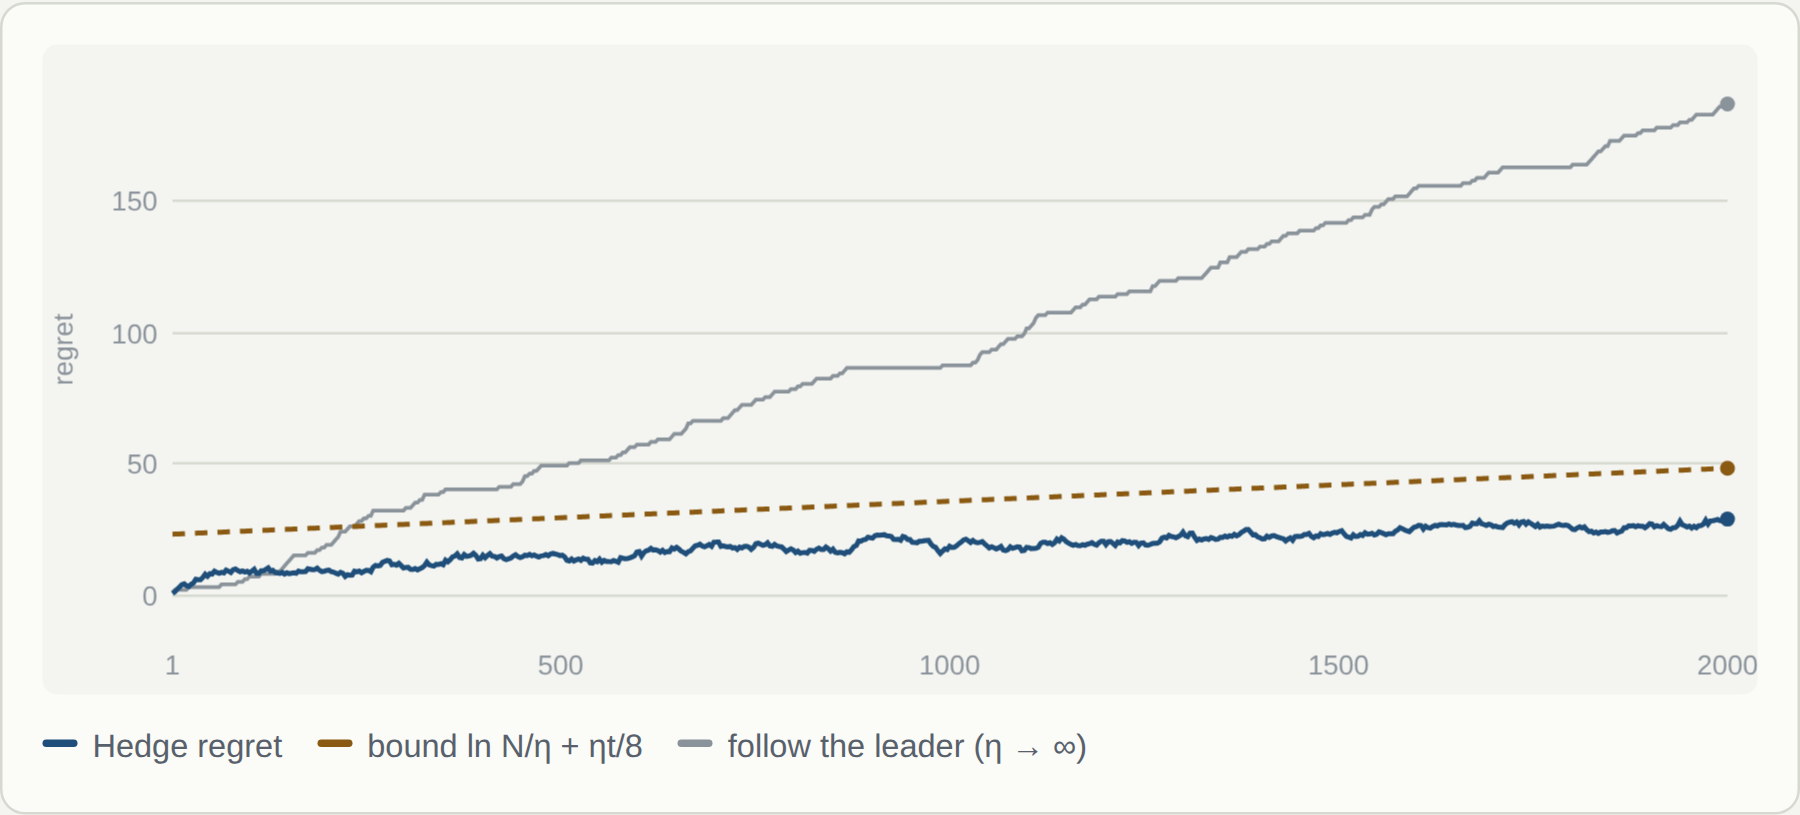
\includegraphics[width=\linewidth]{figures/demo-hedge}
\caption*{\small Simulated market of $N$ signals over $T=2000$ days. Each signal's daily loss is Bernoulli with a mean that drifts; one signal is slightly better on average, and the environment periodically punishes whoever currently leads. Try a very large \ensuremath{\eta} to see Follow the Leader get whipsawed, and a tiny \ensuremath{\eta} to see learning stall. \emph{(A static snapshot at the default settings; the HTML edition has live sliders.)}}
\end{figure}

\section*{3.5 Priors over experts}\addcontentsline{toc}{section}{3.5 Priors over experts}\label{ch3-prior}

Nothing forces uniform initial weights. If we start from $w_{i,1}=\pi_i$ for a prior $\pi\in\simplex_N$, the same proof gives:

\begin{bthm}{Theorem 3.9 \emph{(EWA with a prior)}}

\[\begin{aligned}&L_{\mathrm{MA},T}\\
&\qquad\le\;\frac{\eta L_{i,T}+\ln(1/\pi_i)}{1-e^{-\eta}}\quad\text{and, for Hedge,}\quad \sum_t\ip{p_t}{\ell_t}-L_{i,T}\le\frac{\ln(1/\pi_i)}{\eta}+\frac{\eta T}8.\end{aligned}\]

\end{bthm}

The ``$\ln N$'' was really the description length of the comparator: how many nats it takes to name expert $i$ under the prior. Experts we believe in a priori cost less to compete with. This view has an information-theoretic flavour: regret is the cost of encoding the best expert. It is also exactly what makes infinite or structured expert classes tractable.

\begin{bfin}{In finance}
A fund-of-funds allocator who rebalances capital across $N$ managers each month by multiplying each allocation by $e^{-\eta\cdot(\text{manager's loss})}$ is running Hedge. Theorem 3.8 says: over $T$ months, the allocator's cumulative loss exceeds that of the best single manager by at most $\sqrt{(T/2)\ln N}$, \emph{whatever the markets do}, provided monthly losses are scaled into $[0,1]$. With $N=20$ managers and $T=120$ months, the bound is $\sqrt{60\ln20}\approx13.4$ loss units, or about 0.11 per month. The prior version says a manager you trust more (larger $\pi_i$) is cheaper to track. The catch is the scaling: real returns are unbounded, and a single catastrophic month breaks the $[0,1]$ assumption. Chapter 11 treats multiplicative wealth properly with log-loss.
\end{bfin}

\begin{takeaways}
\begin{itemize}
\item EWA: weights $\propto e^{-\eta\cdot\text{cumulative loss}}$. With convex losses its loss is at most $\frac{\eta L_i+\ln N}{1-e^{-\eta}}$.
\item Hedge: regret $\le\frac{\ln N}\eta+\frac{\eta T}8=\sqrt{(T/2)\ln N}$ at the best $\eta$.
\item With a prior, $\ln N$ becomes $\ln(1/\pi_i)$, the description length of the comparator.
\end{itemize}
\end{takeaways}

\section*{Exercises}\addcontentsline{toc}{section}{Exercises}\label{ch3-ex}

\exercise{3.1}{\extag{easy}{warm-up}}{\hypertarget{sol-3.1}{}Verify that $\nabla\Phi_\eta(L)$ is the Hedge distribution and that $\min_iL_i-\frac{\ln N}\eta\le\Phi_\eta(L)\le\min_iL_i$.}

\exercise{3.2}{\extag{med}{core}}{\hypertarget{sol-3.2}{}(Follow the Leader fails.) Let $N=2$, $\ell_1=(\tfrac12,0)$ and thereafter alternate $(0,1),(1,0),(0,1),\dots$. Show that the algorithm putting all mass on the current leader (ties broken toward expert 1 in round 1) has regret about $T/2$. Which $\eta$ in Hedge corresponds to FTL?}

\exercise{3.3}{\extag{med}{core}}{\hypertarget{sol-3.3}{}Prove Theorem 3.9.}

\exercise{3.4}{\extag{med}{core}}{\hypertarget{sol-3.4}{}(Subsets as experts, from Homework 1.) The experts are all $k$-subsets $S\subseteq[N]$, with loss $\sum_{i\in S}\ell_{i,t}$ (say, the loss of a $k$-stock equally weighted portfolio). Show that EWA's marginal weight $u_i=\sum_{S\ni i}w_S$ can be computed in $O(Nk)$ time, even though there are $\binom Nk$ experts.}

\exercise{3.5}{\extag{hard}{challenge}}{\hypertarget{sol-3.5}{}(Mixability of log loss.) For log loss, show that EWA with $\eta=1$ satisfies $L_{\mathrm{MA},T}\le L_{i,T}+\ln N$, with no $\sqrt T$ term at all. Hint: $e^{-\ell(\hy,y)}=\hy^y(1-\hy)^{1-y}$ and $\hy_t=\sum_ip_{i,t}f_{i,t}$, so $e^{-\ell(\hy_t,y_t)}=\sum_ip_{i,t}e^{-\ell(f_{i,t},y_t)}$.}

\subsection*{Solutions}
\begin{solutions}
\sol{3.1}{$\partial_i\Phi_\eta=\frac{e^{-\eta L_i}}{\sum_je^{-\eta L_j}}$. For the bounds: $e^{-\eta\min L}\le\sum_je^{-\eta L_j}\le Ne^{-\eta\min L}$; apply $-\frac1\eta\ln$.}
\sol{3.2}{After round 1 the leader is expert 2 (loss 0), which then takes loss 1. Now expert 1 leads with 0.5 vs 1, and gets loss 1. The leader always takes the loss of 1, so FTL pays about $T$, while each expert pays about $T/2$. FTL is Hedge with $\eta\to\infty$. Chapter 10 shows that regularization (finite $\eta$) is what stabilises it.}
\sol{3.3}{Now $W_1=\sum_i\pi_i=1$ and $W_{T+1}\ge\pi_ie^{-\eta L_{i,T}}$. The per-round inequality is unchanged. So $(1-e^{-\eta})L_{\mathrm{MA}}\le-\ln W_{T+1}+\ln W_1\le\eta L_{i,T}+\ln(1/\pi_i)$.}
\sol{3.4}{$w_S=\prod_{i\in S}v_i$ with $v_i=e^{-\eta L_i}$, so $\sum_Sw_S=e_k(v)$, the elementary symmetric polynomial. It satisfies the recursion $e_k(v_{1:n})=e_k(v_{1:n-1})+v_ne_{k-1}(v_{1:n-1})$, computable by dynamic programming in $O(nk)$. And $u_i=v_i\,e_{k-1}(v_{-i})$, where $v_{-i}$ drops coordinate $i$. Given the table $e_0(v),\dots,e_k(v)$, the identity $e_j(v)=e_j(v_{-i})+v_i\,e_{j-1}(v_{-i})$ recovers $e_0(v_{-i}),\dots,e_{k-1}(v_{-i})$ in $O(k)$ steps for each $i$, so all marginals cost $O(Nk)$. (In floating point, prefer working in log space or sampling $S$ one element at a time from the DP table.)}
\sol{3.5}{From the hint, $\ell(\hy_t,y_t)=-\ln\frac{W_{t+1}}{W_t}$ exactly. Telescoping gives $L_{\mathrm{MA},T}=-\ln\frac{W_{T+1}}{N}\le L_{i,T}+\ln N$. This is Bayesian model averaging, and it is also the reason Cover's universal portfolio (Chapter 11) has regret logarithmic in $T$.}
\end{solutions}

\chapter[Tracking a moving target]{Tracking a Moving Target: Hyperexperts and Fixed Share}\label{ch4}
\chapsource{Based on Lectures 4–5 (Sept 16 and 18, 2013) · \href{https://web.eecs.umich.edu/~jabernet/eecs598course/fall2013/web/notes/lec5_091813.pdf}{notes 5}}

\begin{goals}
\begin{itemize}
\item Competing against comparators that switch between experts.
\item Why the naive ``all sequences'' prior learns nothing.
\item Fixed Share: a Markov prior over switching sequences, run in $O(N)$ time per round.
\end{itemize}
\end{goals}

\section*{4.1 When the best expert changes}\addcontentsline{toc}{section}{4.1 When the best expert changes}\label{ch4-motivation}

Markets have regimes. A momentum signal may dominate for eighteen months, then a value signal takes over after a crash. Measured against the single best expert over the whole period, Hedge's guarantee is weak in such cases: the best fixed expert may itself be mediocre, and Hedge, having piled weight onto the old leader, may take a long time to move. Indeed, after $T/2$ rounds of expert 1 dominating, expert 2's weight is about $e^{-\eta T/2}$ times smaller, and Hedge needs on the order of another $T/2$ rounds to switch.

The strongest comparator imaginable is the best expert \emph{on each round}, $\sum_t\min_i\ell_{i,t}$. No algorithm can have sublinear regret against it: with two experts and losses $(X_t,1-X_t)$ for random bits $X_t$, every algorithm pays $T/2$ in expectation while the per-round best pays $0$. We need something in between.

\begin{bdef}{Definition 4.1 \emph{(hyperexperts and switches)}}
A \emph{hyperexpert} is a sequence $\mathbf i=(i_1,\dots,i_T)\in[N]^T$ that follows expert $i_t$ on round $t$. Its loss is $L_{\mathbf i}=\sum_t\ell_{i_t,t}$. Its number of switches is $\sigma(\mathbf i)=\abs{\{t<T:i_{t+1}\neq i_t\}}$. \emph{Tracking regret} against the class of hyperexperts with at most $k$ switches is $\sum_t\ip{p_t}{\ell_t}-\min_{\sigma(\mathbf i)\le k}L_{\mathbf i}$.
\end{bdef}

\section*{4.2 A tempting idea that fails}\addcontentsline{toc}{section}{4.2 A tempting idea that fails}\label{ch4-uniform}

There are $N^T$ hyperexperts. Treat each as an expert and run Hedge on them. When we must play a distribution over base experts, we take the marginal: $p_{t,j}\propto v_{t,j}=\sum_{\mathbf i:i_t=j}w_{t,\mathbf i}$.

\begin{bthm}{Claim 4.2}
With uniform initial weights on $[N]^T$, the marginal $p_t$ is uniform on $[N]$ for every $t$, regardless of the losses.
\end{bthm}

\begin{proof}
$w_{t,\mathbf i}=\exp(-\eta\sum_{s<t}\ell_{i_s,s})$ depends only on the prefix $(i_1,\dots,i_{t-1})$. Hence $v_{t,j}=\sum_{i_{1:t-1}}\exp(-\eta\sum_{s<t}\ell_{i_s,s})\cdot N^{T-t}$ for every $j$: the same number.
\end{proof}

Consistent with this, the regret bound $\sqrt{(T/2)\ln N^T}=T\sqrt{(\ln N)/2}$ is linear in $T$ and says nothing. The uniform prior treats a hyperexpert that switches every round as just as plausible as one that never switches, so past data carry no information about the future. The fix is to \emph{put a prior on hyperexperts that prefers few switches}, and use Theorem 3.9.

\section*{4.3 A Markov prior}\addcontentsline{toc}{section}{4.3 A Markov prior}\label{ch4-prior}

\begin{bdef}{Definition 4.3 \emph{(switching prior)}}
Fix $\alpha\in(0,1)$. Draw $i_1$ uniformly. For $t\ge1$, set $i_{t+1}=i_t$ with probability $1-\alpha$; otherwise move to each of the other $N-1$ experts with probability $\frac{\alpha}{N-1}$. Then

\[\Pi(\mathbf i)=\frac1N\Big(\frac{\alpha}{N-1}\Big)^{\sigma(\mathbf i)}(1-\alpha)^{T-1-\sigma(\mathbf i)}.\]

\end{bdef}

By Theorem 3.9, Hedge over hyperexperts with prior $\Pi$ has regret at most $\frac{\ln(1/\Pi(\mathbf i))}{\eta}+\frac{\eta T}{8}$ against every $\mathbf i$, and

\[\ln\frac1{\Pi(\mathbf i)}=\ln N+\sigma\ln\frac{N-1}{\alpha}+(T-1-\sigma)\ln\frac1{1-\alpha}.\]

\begin{bthm}{Theorem 4.4 \emph{(tracking regret)}}
With $\alpha=1/T$, for every hyperexpert with at most $k$ switches, $\ln(1/\Pi(\mathbf i))\le(k+1)\ln(NT)+1$. With $\eta$ tuned for this value,

\[\sum_t\ip{p_t}{\ell_t}-L_{\mathbf i}\;\le\;\sqrt{\tfrac T2\big((k+1)\ln(NT)+1\big)}\;=\;O\big(\sqrt{T\,k\,\ln(NT)}\big).\]

\end{bthm}

\begin{proof}
$\sigma\ln\frac{N-1}{\alpha}\le k\ln(NT)$. For the last term, $\ln\frac1{1-x}\le\frac{x}{1-x}$, so with $x=1/T$, $(T-1-\sigma)\ln\frac{1}{1-1/T}\le(T-1)\cdot\frac1{T-1}=1$. Add $\ln N$ and apply Theorem 3.9 with Lemma 2.5.
\end{proof}

Compare with an oracle that knows where the $k$ switches happen and restarts Hedge on each of the $k+1$ blocks: its regret is $\sum_{b}\sqrt{(T_b/2)\ln N}\le\sqrt{(k+1)(T/2)\ln N}$ by Cauchy–Schwarz. Fixed Share pays only an extra $\ln T$ inside the square root for not knowing the switch times.

\section*{4.4 Fixed Share: the efficient implementation}\addcontentsline{toc}{section}{4.4 Fixed Share: the efficient implementation}\label{ch4-fixedshare}

Maintaining $N^T$ weights is impossible, but the prior is a Markov chain, and marginals of Markov chains can be propagated forward, as in the forward algorithm for hidden Markov models.

\begin{balg}{Algorithm 4.5 \emph{(Fixed Share, Herbster and Warmuth 1998)}}
\begin{algo}
input: \ensuremath{\eta} > 0, \ensuremath{\alpha} \ensuremath{\in} (0,1)
v\_\{j,1\} \ensuremath{\leftarrow} 1/N for all j
for t = 1, 2, …:
    play p\_t = v\_t / \ensuremath{\Sigma}\_j v\_\{t,j\}
    observe \ensuremath{\ell}\_t
    u\_j \ensuremath{\leftarrow} v\_\{t,j\} · exp(\ensuremath{-}\ensuremath{\eta} \ensuremath{\ell}\_\{j,t\})                 \# loss update
    v\_\{t+1,j\} \ensuremath{\leftarrow} (1\ensuremath{-}\ensuremath{\alpha}) u\_j + (\ensuremath{\alpha}/(N\ensuremath{-}1)) \ensuremath{\Sigma}\_\{i\ensuremath{\neq}j\} u\_i    \# share update
\end{algo}

Cost: $O(N)$ per round.
\end{balg}

\begin{bthm}{Proposition 4.6}
Fixed Share plays exactly the marginal distribution of Hedge over hyperexperts with prior $\Pi$. Hence it enjoys Theorem 4.4.
\end{bthm}

\begin{proof}
Let $w_{t,\mathbf i}=\Pi(\mathbf i)\exp(-\eta\sum_{s<t}\ell_{i_s,s})$ and define the prefix weight $\omega_t(i_{1:t})=\Pi(i_{1:t})\exp(-\eta\sum_{s<t}\ell_{i_s,s})$, where $\Pi(i_{1:t})$ is the prior's marginal on the first $t$ coordinates. Summing out future coordinates of a Markov chain gives $v_{t,j}=\sum_{i_{1:t}:\,i_t=j}\omega_t(i_{1:t})$. The Markov property gives the recursion

\[\omega_{t+1}(i_{1:t+1})=\omega_t(i_{1:t})\,e^{-\eta\ell_{i_t,t}}\,P(i_{t+1}\mid i_t).\]

Summing over $i_{1:t}$ with $i_{t+1}=j$ yields $v_{t+1,j}=\sum_iv_{t,i}e^{-\eta\ell_{i,t}}P(j\mid i)$, which is the loss update followed by the share update.
\end{proof}

The share step guarantees every expert keeps weight at least $\frac{\alpha}{N-1}\sum_{i\ne j}u_i$ (at least $\frac{\alpha}{N-1}\sum_iu_i$ whenever $\alpha\le1-\frac1N$, which covers every rate used below), so an expert that was bad for a long time can be picked up within a few rounds once it starts performing. That is precisely the property plain Hedge lacked.

\begin{bfin}{In finance}
Fixed Share is a regime-switching allocator without a regime model. With $N=5$ strategies over $T=2520$ trading days (ten years) and a comparator that switches regimes $k=4$ times, the bound gives roughly $\sqrt{1260\,(5\ln 12600+1)}\approx 246$ loss units, or $0.098$ per day, compared with $0.018$ per day for Hedge against a single fixed strategy. The price of tracking is visible and moderate. In practice $\alpha$ is a ``forgetting rate'': a larger $\alpha$ adapts faster but pays more in stable periods. Choosing it online is itself an experts problem (run Hedge over a grid of $\alpha$ values).
\end{bfin}

\begin{takeaways}
\begin{itemize}
\item Competing with the per-round best is impossible; competing with $k$-switch sequences costs $O(\sqrt{Tk\ln(NT)})$.
\item Uniform priors over huge classes can erase learning. Priors that encode structure are what make large classes useful.
\item A Markov prior lets the exponential-size mixture be computed in $O(N)$ per round.
\end{itemize}
\end{takeaways}

\section*{Exercises}\addcontentsline{toc}{section}{Exercises}\label{ch4-ex}

\exercise{4.1}{\extag{easy}{warm-up}}{\hypertarget{sol-4.1}{}Verify that $\sum_{\mathbf i\in[N]^T}\Pi(\mathbf i)=1$.}

\exercise{4.2}{\extag{med}{core}}{\hypertarget{sol-4.2}{}Show the share update can be written $v_{t+1}=(1-\beta)\,u+\beta\,\frac{\mathbf 1}{N}\sum_iu_i$, and find $\beta$ in terms of $\alpha$ and $N$.}

\exercise{4.3}{\extag{med}{core}}{\hypertarget{sol-4.3}{}Optimise $\alpha$ when $k$ is known. Show that $\alpha=k/(T-1)$ gives $\ln(1/\Pi)\le\ln N+k\ln(N-1)+(T-1)H(\tfrac{k}{T-1})$, where $H$ is binary entropy in nats, and that this is at most $\ln N+k\ln\frac{e(N-1)(T-1)}{k}$.}

\exercise{4.4}{\extag{hard}{challenge}}{\hypertarget{sol-4.4}{}(From Homework 3.) In the portfolio setting of Chapter 11, a ``forgetful'' universal portfolio competes with constant-rebalanced portfolios that change $k$ times. Using the Fixed Share idea, sketch an algorithm and a regret bound of order $(k+1)\,d\ln T$ in log-wealth.}

\subsection*{Solutions}
\begin{solutions}
\sol{4.1}{Group sequences by switch positions and values: there are $N\binom{T-1}{\sigma}(N-1)^\sigma$ sequences with $\sigma$ switches, so the sum is $\sum_\sigma\binom{T-1}{\sigma}\alpha^\sigma(1-\alpha)^{T-1-\sigma}=1$ by the binomial theorem. Or simply note $\Pi$ is the law of a Markov chain.}
\sol{4.2}{$(1-\alpha)u_j+\frac{\alpha}{N-1}(U-u_j)=\big(1-\alpha-\frac{\alpha}{N-1}\big)u_j+\frac{\alpha}{N-1}U$ where $U=\sum_iu_i$. Matching $\frac{\beta}{N}U$ gives $\beta=\frac{\alpha N}{N-1}$, and indeed $1-\beta=1-\alpha-\frac{\alpha}{N-1}$.}
\sol{4.3}{With $\sigma=k$: $k\ln\frac1\alpha+(T-1-k)\ln\frac1{1-\alpha}$ at $\alpha=k/(T-1)$ is exactly $(T-1)H(\alpha)$. Use $H(x)\le x\ln\frac ex$, so $(T-1)H\le k\ln\frac{e(T-1)}k$. This is roughly $\ln\binom{T-1}{k}$, the cost of naming the switch times.}
\end{solutions}

\chapter[Lower bounds]{Lower Bounds: Why $\sqrt{T\ln N}$ Is the Right Answer}\label{ch5}
\chapsource{Based on Lecture 6 (Sept 23, 2013) · \href{https://web.eecs.umich.edu/~jabernet/eecs598course/fall2013/web/notes/lec6_092313.pdf}{scribe notes}}

\begin{goals}
\begin{itemize}
\item Minimax regret as a game between learner and adversary.
\item The probabilistic method: a random adversary is enough to force $\Omega(\sqrt{T\ln N})$ regret.
\end{itemize}
\end{goals}

\section*{5.1 Minimax regret}\addcontentsline{toc}{section}{5.1 Minimax regret}\label{ch5-minimax}

The best guarantee any algorithm can offer is the value of a game in which the learner commits to an algorithm and the adversary then picks the worst loss sequence:

\[V_{T,N}\;=\;\inf_{\text{alg}}\ \sup_{\ell_1,\dots,\ell_T\in[0,1]^N}\Big[\sum_{t=1}^T\ip{p_t}{\ell_t}-\min_i\sum_{t=1}^T\ell_{i,t}\Big].\]

Hedge shows $V_{T,N}\le\sqrt{(T/2)\ln N}$. To show no algorithm does much better, we use the trick that \emph{a maximum is at least an average}: replace the worst-case adversary by a random one, and show that \emph{every} algorithm has large expected regret against it.

\section*{5.2 Two experts}\addcontentsline{toc}{section}{5.2 Two experts}\label{ch5-two}

Let $X_1,\dots,X_T$ be independent fair coin flips and set $\ell_t=(X_t,1-X_t)$.

\begin{proof}[Argument]
\begin{enumerate}
\item Since $p_t$ depends only on $X_{1:t-1}$, and $\E[\ell_t\mid X_{1:t-1}]=(\tfrac12,\tfrac12)$, we get $\E\ip{p_t}{\ell_t}=\tfrac12$ for every algorithm. The learner's expected loss is exactly $T/2$, whatever it does.
\item So $V_{T,2}\ge\E\big[\tfrac T2-\min(S,T-S)\big]$ with $S=\sum_tX_t$, and $\tfrac T2-\min(S,T-S)=\abs{S-\tfrac T2}$.
\item With Rademacher signs $Z_t=2X_t-1$, this is $\tfrac12\E\abs{\sum_tZ_t}$.
\item By the central limit theorem, $\E\abs{\sum_tZ_t}\sim\sqrt{T}\,\E\abs{G}=\sqrt{2T/\pi}$ for $G\sim\mathcal N(0,1)$.
\end{enumerate}

Hence $V_{T,2}\ge\sqrt{T/(2\pi)}\,(1+o(1))$.
\end{proof}

The adversary did nothing clever: pure noise suffices. The learner cannot predict a coin, and in hindsight one of the two experts will have been lucky by about $\sqrt T$. Regret measures that luck.

\section*{5.3 $N$ experts}\addcontentsline{toc}{section}{5.3 $N$ experts}\label{ch5-N}

For even $N$, use $N/2$ independent pairs: $\ell_t=(X^1_t,1-X^1_t,\dots,X^{N/2}_t,1-X^{N/2}_t)$. The learner still pays $T/2$ in expectation, and

\[V_{T,N}\;\ge\;\tfrac12\,\E\max_{j\le N/2}\Big\lvert\sum_tZ^j_t\Big\rvert\;\approx\;\tfrac12\sqrt T\;\E\max_{j\le N/2}\abs{G_j}\;\approx\;\tfrac12\sqrt{T}\sqrt{2\ln(N/2)}.\]

The last step uses the fact that the maximum of $n$ independent standard Gaussians concentrates around $\sqrt{2\ln n}$. A sharper version, using $N$ independent (not paired) experts, gives the exact constant.

\begin{bthm}{Theorem 5.1 \emph{(Cesa-Bianchi and Lugosi 2006, Thm 3.7)}}

\[\lim_{N\to\infty}\ \lim_{T\to\infty}\ \frac{V_{T,N}}{\sqrt{(T/2)\ln N}}\;=\;1.\]

\end{bthm}

So Hedge with a tuned learning rate is \emph{asymptotically optimal including the constant}, a rare situation in learning theory.

\section*{5.4 Regret as a game}\addcontentsline{toc}{section}{5.4 Regret as a game}\label{ch5-game}

This chapter used the adversary's randomness to lower-bound a min-max. Exchanging the order of play is the subject of the minimax theorem in the next chapter, and in Part VI we will see that the learner's side of the game can also be treated geometrically. It is worth noting now that lower bounds in online learning often come from a stochastic adversary, while upper bounds hold for adversarial sequences. When the two match, as here, stochastic data are as hard as adversarial data, and the adversarial model costs nothing in the worst case.

\begin{bfin}{In finance}
If daily signal performance is indistinguishable from coin flips, which is roughly the efficient-markets null, then the best signal in a library of $N$ will beat the coin-flip average by about $\sqrt{(T/2)\ln N}$ loss units just by luck. This is the online-learning version of the data-snooping problem (White, 2000; Harvey, Liu and Zhu, 2016): the best backtest in a large library is biased upward by that amount, and any strategy that selects signals online will trail that best backtest by roughly the same amount. Theorem 5.1 says no allocation rule can beat this, which is a principled haircut to apply to backtested Sharpe ratios.
\end{bfin}

\begin{takeaways}
\begin{itemize}
\item A random adversary lower-bounds the worst case. Against i.i.d. coin-flip losses every learner pays $T/2$ in expectation.
\item The best of $N$ random walks gets ahead by about $\sqrt{2T\ln N}$ steps, i.e. $\sqrt{(T/2)\ln N}$ in loss units, which forces regret $\Omega(\sqrt{T\ln N})$.
\item Hedge's $\sqrt{(T/2)\ln N}$ is optimal, constant included.
\end{itemize}
\end{takeaways}

\section*{Exercises}\addcontentsline{toc}{section}{Exercises}\label{ch5-ex}

\exercise{5.1}{\extag{easy}{warm-up}}{\hypertarget{sol-5.1}{}Show that for $n$ i.i.d. standard Gaussians, $\E\max_jG_j\le\sqrt{2\ln n}$. Hint: for $\lambda>0$, $e^{\lambda\E\max G}\le\E e^{\lambda\max G}\le\sum_j\E e^{\lambda G_j}=ne^{\lambda^2/2}$.}

\exercise{5.2}{\extag{med}{core}}{\hypertarget{sol-5.2}{}For $T=4$, compute $\E\abs{\sum_{t\le4}Z_t}$ exactly and compare with $\sqrt{2T/\pi}$.}

\exercise{5.3}{\extag{hard}{challenge}}{\hypertarget{sol-5.3}{}Show that the bound of Chapter 4 is also tight up to logarithmic factors: any algorithm has tracking regret $\Omega(\sqrt{Tk\ln N})$ against $k$-switch comparators. Hint: split time into $k+1$ blocks and apply the $N$-expert lower bound in each.}

\subsection*{Solutions}
\begin{solutions}
\sol{5.1}{Taking logs, $\E\max G\le\frac{\ln n}{\lambda}+\frac\lambda2$. Minimise at $\lambda=\sqrt{2\ln n}$. This is the same balancing as in Hedge, and it is no coincidence: the proof of Hedge is a deterministic version of this argument.}
\sol{5.2}{$\sum Z\in\{-4,-2,0,2,4\}$ with probabilities $\frac1{16},\frac4{16},\frac6{16},\frac4{16},\frac1{16}$. $\E\abs{\cdot}=\frac{2(4\cdot1+2\cdot4)}{16}=1.5$. $\sqrt{8/\pi}\approx1.60$.}
\end{solutions}

\def\thepartblurb{No-regret learning proves the minimax theorem, computes equilibria, solves linear programs and boosts weak classifiers.}\part{Games, Equilibria and Their Uses}\label{part2}

\chapter[Zero-sum games and minimax]{Zero-Sum Games and the Minimax Theorem}\label{ch6}
\chapsource{Based on Lectures 6–8 (Sept 23 – 30, 2013) · \href{https://web.eecs.umich.edu/~jabernet/eecs598course/fall2013/web/notes/lec7_092513.pdf}{notes 7} · \href{https://web.eecs.umich.edu/~jabernet/eecs598course/fall2013/web/notes/lec8_093013.pdf}{notes 8}}

\begin{goals}
\begin{itemize}
\item Bimatrix games, mixed strategies, best responses and Nash equilibria.
\item Nash's existence theorem via Brouwer.
\item Von Neumann's minimax theorem, proved by letting two Hedge players play each other.
\end{itemize}
\end{goals}

\section*{6.1 Games in normal form}\addcontentsline{toc}{section}{6.1 Games in normal form}\label{ch6-games}

\begin{bdef}{Definition 6.1 \emph{(bimatrix game)}}
A two-player game is a pair of $n\times m$ matrices $(A,B)$. The row player picks $i\in[n]$ and receives $A_{ij}$; the column player picks $j\in[m]$ and receives $B_{ij}$. Mixed strategies $x\in\simplex_n$, $y\in\simplex_m$ give expected payoffs $x^\top Ay$ and $x^\top By$. The game is \textbf{zero-sum} if $B=-A$.
\end{bdef}

\begin{bexample}{Example 6.2 \emph{(Prisoners' Dilemma)}}
Actions: confess (1) or stay silent (2). Payoffs are minus years in prison:

\[A=\begin{pmatrix}-8&0\\-10&-1\end{pmatrix},\qquad B=A^\top=\begin{pmatrix}-8&-10\\0&-1\end{pmatrix}.\]

Confessing is better for each player whatever the other does: $-8>-10$ and $0>-1$. So (confess, confess) is the unique equilibrium, with payoff $(-8,-8)$, although (silent, silent) gives both players $-1$. Individually rational play can be collectively bad.
\end{bexample}

\begin{bexample}{Example 6.3 \emph{(penalty kicks)}}
The kicker (rows) aims left or right and the goalie (columns) dives left or right. The kicker scores unless the goalie guesses right, so with payoff $+1$ for a goal the kicker gets $A=\begin{pmatrix}-1&1\\1&-1\end{pmatrix}$ and $B=-A$. Here, every pure pair has a player who wants to deviate. The only equilibrium is both players mixing $(\tfrac12,\tfrac12)$, with value $0$.
\end{bexample}

\begin{bdef}{Definition 6.4 \emph{(best response, Nash equilibrium)}}
$\mathrm{BR}_1(y)=\argmax_{x\in\simplex_n}x^\top Ay$ and $\mathrm{BR}_2(x)=\argmax_{y\in\simplex_m}x^\top By$. Because payoffs are linear in one's own strategy, a pure best response always exists. A pair $(x^*,y^*)$ is a \textbf{Nash equilibrium} if $x^*\in\mathrm{BR}_1(y^*)$ and $y^*\in\mathrm{BR}_2(x^*)$; equivalently, neither player regrets their choice against any pure deviation: $x^{*\top}Ay^*\ge e_i^\top Ay^*$ for all $i$ and $x^{*\top}By^*\ge x^{*\top}Be_j$ for all $j$. It is an \textbf{$\eps$-equilibrium} if each inequality holds up to $\eps$.
\end{bdef}

\section*{6.2 Nash's theorem}\addcontentsline{toc}{section}{6.2 Nash's theorem}\label{ch6-nash}

\begin{bthm}{Theorem 6.5 \emph{(Nash 1950)}}
Every finite bimatrix game has at least one mixed Nash equilibrium.
\end{bthm}

The proof uses Brouwer's fixed-point theorem: every continuous map from a compact convex set to itself has a fixed point.

\begin{proof}
Define the gains from deviating, $c_i(x,y)=\max(0,e_i^\top Ay-x^\top Ay)$ and $d_j(x,y)=\max(0,x^\top Be_j-x^\top By)$, and the map $f(x,y)=(x',y')$ with

\[x'_i=\frac{x_i+c_i}{1+\sum_kc_k},\qquad y'_j=\frac{y_j+d_j}{1+\sum_kd_k}.\]

$f$ is continuous and maps $\simplex_n\times\simplex_m$ into itself, so it has a fixed point $(x,y)$. Some $k$ with $x_k>0$ has $e_k^\top Ay\le x^\top Ay$ (an average cannot be strictly below every term in its support), so $c_k=0$. At the fixed point $x_k=\frac{x_k}{1+\sum_ic_i}$, which forces $\sum_ic_i=0$. The same argument gives $\sum_jd_j=0$. So nobody gains from deviating.
\end{proof}

The proof is not constructive, and indeed computing a Nash equilibrium of a general bimatrix game is PPAD-complete (Chen and Deng 2006; Daskalakis, Goldberg and Papadimitriou 2006). The zero-sum case is different: equilibria are computable efficiently, and no-regret learning finds them.

\section*{6.3 Von Neumann's minimax theorem}\addcontentsline{toc}{section}{6.3 Von Neumann's minimax theorem}\label{ch6-minimax}

From here on, $M\in[0,1]^{n\times m}$ is a loss matrix: the row player chooses $p\in\simplex_n$ to \emph{minimise} $p^\top Mq$, and the column player chooses $q\in\simplex_m$ to maximise it.

\begin{bthm}{Theorem 6.6 \emph{(von Neumann 1928)}}

\[\min_{p\in\simplex_n}\max_{q\in\simplex_m}p^\top Mq\;=\;\max_{q\in\simplex_m}\min_{p\in\simplex_n}p^\top Mq\;=:\;V.\]

\end{bthm}

The inequality $\min\max\ge\max\min$ is easy: on the left the maximiser moves second and can react to $p$; moving second never hurts. The content of the theorem is the reverse: in zero-sum games \emph{announcing your mixed strategy costs nothing}. There is a $p^*$ with $p^{*\top}Mq\le V$ for every $q$, and a $q^*$ with $p^\top Mq^*\ge V$ for every $p$.

\begin{bthm}{Proof via no-regret learning}
Let the row player run Hedge on loss vectors $\ell_t=Mq_t$, and let the column player run any no-regret algorithm on gain vectors $g_t=M^\top p_t$ (Hedge on gains: $w_{j}\leftarrow w_je^{\eta g_{j,t}}$). Write $\bar p=\frac1T\sum_tp_t$, $\bar q=\frac1T\sum_tq_t$, and $\eps_T=\Reg_T/T=O(\sqrt{\ln(\max(n,m))/T})$.
\end{bthm}

\begin{proof}
The row player's regret bound gives

\[\frac1T\sum_tp_t^\top Mq_t\;\le\;\min_p\frac1T\sum_tp^\top Mq_t+\eps_T\;=\;\min_pp^\top M\bar q+\eps_T\;\le\;\max_q\min_pp^\top Mq+\eps_T.\]

The column player's regret bound gives

\[\frac1T\sum_tp_t^\top Mq_t\;\ge\;\max_q\bar p^\top Mq-\eps_T\;\ge\;\min_p\max_qp^\top Mq-\eps_T.\]

Chaining, $\min\max\le\max\min+2\eps_T$. Let $T\to\infty$.
\end{proof}

The proof gives more than the theorem:

\begin{bthm}{Corollary 6.7 \emph{(equilibrium computation by self-play)}}
The average strategies form a $2\eps_T$-equilibrium: $\max_q\bar p^\top Mq\le V+2\eps_T$ and $\min_pp^\top M\bar q\ge V-2\eps_T$. With Hedge on both sides, $T=O(\ln(nm)/\eps^2)$ rounds suffice for an $\eps$-equilibrium, each costing $O(nm)$ arithmetic. If the column player instead \emph{best-responds}, $q_t\in\argmax_qp_t^\top Mq$, it has non-positive regret and the guarantee improves to $\eps_T$.
\end{bthm}

Note that it is the \emph{averages} $\bar p,\bar q$ that converge. The day-to-day strategies $p_t,q_t$ of two Hedge players typically cycle around the equilibrium without settling. More recent ``optimistic'' variants of Hedge, which add a guess of the next loss to the cumulative loss, converge faster: their averages converge at rate $O(\ln T/T)$ (Daskalakis, Deckelbaum and Kim 2011; Rakhlin and Sridharan 2013) and even $O(1/T)$ (Syrgkanis, Agarwal, Luo and Schapire 2015), and the last iterate itself converges (Daskalakis and Panageas 2019; Wei, Lee, Zhang and Luo 2021).

\begin{bwarn}{Fictitious play}
If both players use Follow the Leader (best response to the opponent's empirical average), we get Brown's fictitious play. Robinson (1951) proved it converges in zero-sum games, but with the rate $T^{-1/(n+m-2)}$. Karlin conjectured the rate is really $O(T^{-1/2})$, as simulations suggest. Daskalakis and Pan (2014) disproved the conjecture when ties are broken adversarially; with consistent tie-breaking it remains open. This is Homework 2, Problem 3(b).
\end{bwarn}

\section*{6.4 Minimax and linear programming}\addcontentsline{toc}{section}{6.4 Minimax and linear programming}\label{ch6-lp}

The value of a zero-sum game is a linear program. Because $\max_q$ of a linear function is attained at a vertex,

\[V=\min_{c\in\R,\,p\in\simplex_n}c\quad\text{subject to}\quad(p^\top M)_j\le c\ \ \text{for } j=1,\dots,m.\]

Its LP dual is the max-min problem, so LP strong duality implies the minimax theorem. The converse also holds, in the sense that any LP can be reduced to a zero-sum game (Dantzig 1951; Adler 2013). The link is the Lagrangian: $\max_{x\ge0}\{d^\top x:Ax\le b\}=\max_{x\ge0}\min_{y\ge0}\,d^\top x+y^\top(b-Ax)$, and exchanging max and min gives the dual $\min_{y\ge0}\{b^\top y:A^\top y\ge d\}$. Chapter 7 uses this to solve LPs with Hedge.

\begin{bfin}{In finance}
Robust portfolio choice is a zero-sum game against nature: the investor picks weights $p$, nature picks a scenario $j$, and the loss is $M_{\cdot j}$. The minimax theorem says the investor's worst-case-optimal mix $p^*$ is also a best response to a \emph{least-favourable prior} $q^*$ over scenarios. That is the mathematical content behind the claim that robust optimisation is Bayesian optimisation under a pessimistic prior. Self-play Hedge computes both $p^*$ and $q^*$ for scenario sets far too large for an off-the-shelf LP solver to handle comfortably, since the iteration count scales only with $\ln m$.
\end{bfin}

\begin{takeaways}
\begin{itemize}
\item Nash equilibria exist (Brouwer) but are hard to compute in general.
\item In zero-sum games $\min\max=\max\min$. Two no-regret learners playing each other converge on average to an equilibrium, at rate $2\Reg_T/T$.
\item Minimax duality and LP duality are two views of the same fact.
\end{itemize}
\end{takeaways}

\section*{Exercises}\addcontentsline{toc}{section}{Exercises}\label{ch6-ex}

\exercise{6.1}{\extag{easy}{warm-up}}{\hypertarget{sol-6.1}{}Find the value and optimal strategies of $M=\begin{pmatrix}0.2&0.7\\0.6&0.3\end{pmatrix}$ (row player minimises).}

\exercise{6.2}{\extag{med}{core}}{\hypertarget{sol-6.2}{}Prove that in a zero-sum game the set of equilibria is a product $P^*\times Q^*$ of convex sets, and all equilibria have the same value. Show this fails for the general-sum game of Example 6.2 modified so that there are two equilibria with different payoffs (for example, a coordination game).}

\exercise{6.3}{\extag{med}{core}}{\hypertarget{sol-6.3}{}(Regularized best responses, from Lecture 8.) Replace best responses by $x'=\argmax_x\{x^\top Ay-\eps\norm{x}^2\}$ and similarly for $y$. Show this map is continuous, that any fixed point is an $\eps$-equilibrium, and deduce Nash's theorem by letting $\eps\to0$.}

\exercise{6.4}{\extag{hard}{project}}{\hypertarget{sol-6.4}{}(Homework 2, Problem 3.) For $M=\begin{pmatrix}5&8&3&1&6\\4&2&6&3&5\\2&4&6&4&1\\1&3&2&5&3\end{pmatrix}$, run for $T=10^4$ rounds: (i) Hedge vs Hedge; (ii) Hedge vs best response; (iii) FTPL vs FTPL with fresh perturbations; (iv) fictitious play. Plot the duality gap $\max_j\bar p^\top Me_j-\min_ie_i^\top M\bar q$ against $T$ on log-log axes. Which method converges fastest in practice?}

\exercise{6.5}{\extag{hard}{challenge}}{\hypertarget{sol-6.5}{}(Homework 3, Problem 1.) Let $X,Y$ be convex compact sets and $f(x,y)$ convex in $x$, concave in $y$, with bounded gradients. Prove $\inf_x\sup_yf=\sup_y\inf_xf$ by letting both players run online gradient descent (Chapter 9), and show that the averaged iterates form an $\eps$-saddle point after $O(1/\eps^2)$ rounds.}

\subsection*{Solutions}
\begin{solutions}
\sol{6.1}{No saddle point, so both mix. The row player equalises columns: $0.2p+0.6(1-p)=0.7p+0.3(1-p)$, so $0.6-0.4p=0.3+0.4p$, $p=3/8$. Value $=0.6-0.15=0.45$. The column player equalises rows: $0.2q+0.7(1-q)=0.6q+0.3(1-q)$, so $0.7-0.5q=0.3+0.3q$, $q=1/2$, value $0.45$.}
\sol{6.2}{$(p,q)$ is an equilibrium iff $p\in P^*=\{p:\max_qp^\top Mq=V\}$ and $q\in Q^*=\{q:\min_pp^\top Mq=V\}$, by the minimax theorem. Each set is a sublevel/superlevel set of a convex/concave function, hence convex. In the coordination game $A=B=\mathrm{diag}(2,1)$, both $(1,1)$ and $(2,2)$ are equilibria, with payoffs 2 and 1, and mixing them is not an equilibrium.}
\sol{6.3}{The objective is strictly concave, so the maximiser is unique, and by Berge's maximum theorem it varies continuously in $y$. At a fixed point $x$ maximises $x^\top Ay-\eps\norm x^2$, and $0\le\norm{x}^2\le1$ on the simplex, so $x^\top Ay\ge e_i^\top Ay-\eps$. Take $\eps_k\to0$; by compactness a subsequence of fixed points converges, and the limit satisfies the equilibrium inequalities by continuity. Using $\ln$-entropy instead of $\norm x^2$ gives ``logit'' or quantal-response equilibria, with softmax best responses: Hedge's update rule.}
\sol{6.5}{Player $x$ runs OGD on $f_t(x)=f(x,y_t)$, player $y$ runs OGD on $-f(x_t,y)$. Both regrets are $O(\sqrt T)$. Exactly as in §6.3, convexity (Jensen) in $x$ and concavity in $y$ give $\sup_yf(\bar x,y)\le\frac1T\sum_tf(x_t,y_t)+\frac{R_T}T\le\inf_xf(x,\bar y)+\frac{2R_T}T$.}
\end{solutions}

\chapter[Linear programs and boosting]{Applications of Minimax: Linear Programs and Boosting}\label{ch7}
\chapsource{Based on Lectures 9–10 (Oct 2 and 7, 2013) · \href{https://web.eecs.umich.edu/~jabernet/eecs598course/fall2013/web/notes/lec9_100213.pdf}{notes 9} · \href{https://web.eecs.umich.edu/~jabernet/eecs598course/fall2013/web/notes/lec10_100713.pdf}{notes 10}}

\begin{goals}
\begin{itemize}
\item A multiplicative-weights solver for LP feasibility whose iteration count ignores the number of constraints.
\item Boosting: why weak learners can always be combined into a strong one (minimax), and how to find the combination (Hedge).
\end{itemize}
\end{goals}

\section*{7.1 Solving linear programs with Hedge}\addcontentsline{toc}{section}{7.1 Solving linear programs with Hedge}\label{ch7-lp}

Any bounded LP can be put in a normalised feasibility form. First add $\sum_ix_i=1$ (rescale, adding a slack coordinate if necessary), which makes $x\in\simplex_n$. Then $a_j^\top x\le b_j$ becomes $(a_j-b_j\mathbf1)^\top x\le0$. An objective $c^\top x\ge d$ becomes one more constraint $(d\mathbf1-c)^\top x\le0$, and binary search on $d$ recovers optimisation at a cost of a $\log(1/\eps)$ factor.

\begin{bdef}{Problem 7.1 \emph{(approximate LP feasibility)}}
Given vectors $\{a_j\}_{j\in J}\subset[-\rho,\rho]^n$, either find $x\in\simplex_n$ with $a_j^\top x\le\eps$ for all $j$, or certify that no $x\in\simplex_n$ has $a_j^\top x\le0$ for all $j$.
\end{bdef}

View it as a game: the $x$-player picks a mixture of coordinates, and an adversary answers with the most violated constraint.

\begin{balg}{Algorithm 7.2 \emph{(multiplicative-weights LP)}}
\begin{algo}
x\_1 \ensuremath{\leftarrow} uniform on [n]
for t = 1, …, T:
    j\_t \ensuremath{\leftarrow} argmax\_j  a\_j\ensuremath{^{\top}} x\_t                 \# most violated constraint (an "oracle")
    if a\_\{j\_t\}\ensuremath{^{\top}} x\_t \ensuremath{\le} \ensuremath{\varepsilon}:  return x\_t
    x\_\{t+1,i\} \ensuremath{\propto} x\_\{t,i\} · exp(\ensuremath{-}\ensuremath{\eta} a\_\{j\_t,i\})   \# Hedge on loss vector a\_\{j\_t\}
return INFEASIBLE
\end{algo}
\end{balg}

\begin{bthm}{Theorem 7.3}
With $T>\frac{2\rho^2\ln n}{\eps^2}$ and the matching $\eta$, Algorithm 7.2 is correct.
\end{bthm}

\begin{proof}
Loss vectors lie in $[-\rho,\rho]^n$, a range of $2\rho$, so Hedge's regret is at most $\rho\sqrt{2T\ln n}$ (Theorem 3.8 rescaled). Suppose a feasible $x^\circ$ exists but the algorithm returns INFEASIBLE. Every round had $a_{j_t}^\top x_t>\eps$, so

\[\begin{aligned}&\eps\;<\;\frac1T\sum_ta_{j_t}^\top x_t\;\le\;\frac1T\sum_ta_{j_t}^\top x^\circ+\rho\sqrt{\frac{2\ln n}{T}}\\
&\qquad\le\;0+\rho\sqrt{\frac{2\ln n}{T}},\end{aligned}\]

which contradicts the choice of $T$.
\end{proof}

The iteration count depends on the dimension only through $\ln n$ and not at all on the number of constraints $\abs{J}$, which may be exponential as long as we can find the most violated one. This is the Plotkin–Shmoys–Tardos framework; Arora, Hazan and Kale (2012) survey its many uses, from multicommodity flow to semidefinite programming. The price is the $1/\eps^2$ dependence, which makes it a tool for fast, low-precision solutions.

\begin{bfin}{In finance: finding a pricing measure}
Suppose $S$ states of the world, and $m$ traded assets with discounted payoff vectors $\pi_j\in\R^S$ and prices $c_j$. By the fundamental theorem of asset pricing (in its one-period, finite-state form), there is no arbitrage iff there is a strictly positive state-price vector, i.e. a risk-neutral measure $q\in\simplex_S$ with $q^\top\pi_j=c_j$ for all $j$. Writing each equality as two inequalities $\pm(\pi_j-c_j\mathbf 1)^\top q\le0$ gives Problem 7.1 (up to strict positivity, which the approximate solver does not enforce). Algorithm 7.2 either returns an approximately consistent pricing measure over, say, $S=10^6$ scenario states in $O(\rho^2\ln S/\eps^2)$ rounds, or its failure certifies (through LP duality) a portfolio that is an $\eps$-arbitrage. The Hedge weights over states behave like a Gibbs or maximum-entropy pricing measure, which connects to the entropy-based calibration of option surfaces used in practice (Avellaneda's weighted Monte Carlo).
\end{bfin}

\section*{7.2 Boosting}\addcontentsline{toc}{section}{7.2 Boosting}\label{ch7-boost}

Can a learner that is only slightly better than guessing be turned into one that is accurate? Kearns and Valiant asked this in 1988; Schapire (1990) and Freund and Schapire (1997, AdaBoost) answered yes. The game-theoretic view makes the answer almost immediate.

\begin{bdef}{Setup}
Training points $x_1,\dots,x_N$ with labels $c(x_i)\in\{0,1\}$; a class $\mathcal H$ of base hypotheses (for example decision stumps $h_{k,\theta}(x)=\ind[x_k\ge\theta]$). Define the $N\times\abs{\mathcal H}$ matrix

\[M_{i,h}=\begin{cases}+1&h(x_i)\neq c(x_i)\\-1&h(x_i)=c(x_i).\end{cases}\]

For a distribution $p$ over points, $p^\top Me_h=2\Pr_{i\sim p}[h\text{ errs}]-1$.
\end{bdef}

\begin{bdef}{Definition 7.4 \emph{(weak learning assumption, WLA$_\gamma$)}}
For every distribution $p$ over the training points there is $h\in\mathcal H$ with $\Pr_{i\sim p}[h(x_i)\neq c(x_i)]\le\frac12-\frac\gamma2$, i.e. $p^\top Me_h\le-\gamma$.
\end{bdef}

\begin{bthm}{Theorem 7.5 \emph{(weak implies strong)}}
Under WLA$_\gamma$ there is a distribution $q$ over $\mathcal H$ whose weighted majority vote is correct on every training point, with margin $\gamma$: $e_i^\top Mq\le-\gamma$ for all $i$.
\end{bthm}

\begin{proof}
WLA$_\gamma$ says $\max_p\min_qp^\top Mq\le-\gamma$. By the minimax theorem, $\min_q\max_pp^\top Mq\le-\gamma$, so some $q$ has $e_i^\top Mq\le-\gamma$ for every point $i$. For point $i$ that means the $q$-weight of hypotheses that err is at most $\frac12-\frac\gamma2$, so the weighted vote is right.
\end{proof}

Existence is not enough; we want to find $q$ with few calls to the weak learner. Let the \emph{data player} run Hedge to find distributions on which the current ensemble is weak, and let the weak learner best-respond.

\begin{balg}{Algorithm 7.6 \emph{(boosting by Hedge)}}
\begin{algo}
p\_1 \ensuremath{\leftarrow} uniform over the N training points
for t = 1, …, T:
    h\_t \ensuremath{\leftarrow} WeakLearner(p\_t)          \# error under p\_t \ensuremath{\le} ½ \ensuremath{-} \ensuremath{\gamma}/2
    for each i:  p\_\{t+1,i\} \ensuremath{\propto} p\_\{t,i\} · exp(\ensuremath{\eta} M\_\{i,h\_t\})
                 \# up-weight points h\_t got wrong, down-weight the rest
output majority vote of h\_1, …, h\_T
\end{algo}
\end{balg}

\begin{bthm}{Theorem 7.7}
If $T>\frac{2\ln N}{\gamma^2}$, the majority vote of $h_1,\dots,h_T$ classifies every training point correctly.
\end{bthm}

\begin{proof}
The data player gains $g_t=Me_{h_t}\in[-1,1]^N$ and has regret at most $\sqrt{2T\ln N}$. So for every $i$,

\[\frac1T\sum_tM_{i,h_t}\;\le\;\frac1T\sum_tp_t^\top Me_{h_t}+\sqrt{\frac{2\ln N}{T}}\;\le\;-\gamma+\sqrt{\frac{2\ln N}{T}}\;<\;0.\]

The left side is (fraction of $h_t$ wrong on $x_i$) minus (fraction right), so the majority is right on $x_i$.
\end{proof}

AdaBoost is this algorithm with a round-dependent step $\eta_t=\frac12\ln\frac{1-\eps_t}{\eps_t}$ (where $\eps_t$ is $h_t$'s weighted error) and a weighted rather than plain majority vote. It adapts to each round's actual edge, and its training error is at most $\prod_t\sqrt{1-\gamma_t^2}\le\exp(-\frac12\sum_t\gamma_t^2)$ where $\gamma_t=1-2\eps_t$. Generalisation beyond the training set follows from margin theory (Schapire, Freund, Bartlett and Lee 1998): the vote's large margin $\gamma$ controls test error independently of $T$.

\begin{bfin}{In finance}
Boosted stumps and trees (AdaBoost, gradient boosting, XGBoost) are among the most common models for cross-sectional return prediction and credit scoring. The game view explains one of their failure modes in finance. The data player concentrates weight on the hardest examples, and in return data those are often outliers or mislabelled events (a stock split read as a crash). Boosting will spend its capacity fitting them. Robust variants cap the weights (the ``smooth boosting'' of Servedio), which in game terms restricts the data player to smooth distributions.
\end{bfin}

\begin{takeaways}
\begin{itemize}
\item Hedge solves LP feasibility to accuracy $\eps$ in $O(\rho^2\ln n/\eps^2)$ rounds, independent of the number of constraints.
\item Weak learnability for every distribution means (by minimax) that one mixture of weak hypotheses is strong.
\item Boosting is Hedge on training points against a best-responding weak learner. $O(\ln N/\gamma^2)$ rounds suffice.
\end{itemize}
\end{takeaways}

\section*{Exercises}\addcontentsline{toc}{section}{Exercises}\label{ch7-ex}

\exercise{7.1}{\extag{med}{core}}{\hypertarget{sol-7.1}{}Show that the converse of Theorem 7.5 holds: if some mixture $q$ has margin $\gamma$ on every point, then WLA$_\gamma$ holds.}

\exercise{7.2}{\extag{med}{core}}{\hypertarget{sol-7.2}{}Derive AdaBoost's step size: with weights $p_t$ and weak error $\eps_t$, find the $\eta$ that minimises the normaliser $Z_t=\sum_ip_{t,i}e^{\eta M_{i,h_t}}$ (correct points, with $M_{i,h_t}=-1$, are down-weighted), and show $\min_\eta Z_t=2\sqrt{\eps_t(1-\eps_t)}$.}

\exercise{7.3}{\extag{fin}{finance}}{\hypertarget{sol-7.3}{}Three states, a bond paying $(1,1,1)$ at price $1$, a stock paying $(0.8,1,1.3)$ at price $1$, and a call on the stock struck at $1$ paying $(0,0,0.3)$. For which call prices $c$ is there no arbitrage? Run the first iteration of Algorithm 7.2 by hand with $c=0.1$, and say what the second will do.}

\subsection*{Solutions}
\begin{solutions}
\sol{7.1}{For any $p$, $p^\top Mq=\sum_ip_ie_i^\top Mq\le-\gamma$. Since $p^\top Mq$ is an average of $p^\top Me_h$ over $h\sim q$, some $h$ has $p^\top Me_h\le-\gamma$. So weak and strong learnability (with margins) are equivalent: this is minimax duality.}
\sol{7.2}{$Z(\eta)=\eps_te^{\eta}+(1-\eps_t)e^{-\eta}$. Setting $Z'=0$: $e^{2\eta}=\frac{1-\eps_t}{\eps_t}$, so $\eta=\frac12\ln\frac{1-\eps_t}{\eps_t}$ and $Z=2\sqrt{\eps_t(1-\eps_t)}=\sqrt{1-\gamma_t^2}$. The training error is at most $\prod_tZ_t$ because the exponential loss upper-bounds the 0/1 loss.}
\sol{7.3}{We need $q\in\simplex_3$ with $0.8q_1+q_2+1.3q_3=1$ and $0.3q_3=c$. From the stock equation, $0.3q_3=0.2q_1$, so $q_1=1.5q_3$ and $q_2=1-2.5q_3$. Strict positivity needs $0<q_3<0.4$, so $c=0.3q_3\in(0,0.12)$. For $c=0.1$: $q_3=1/3$, $q_1=1/2$, $q_2=1/6$. Starting from uniform $q$, the stock constraint $(-0.2,0,0.3)^\top q=0.033>0$ is violated (the others give $0$ and $-0.033$), so Hedge moves weight from state 3 toward state 1: with $\eta=1$, $q_2\propto(e^{0.2},1,e^{-0.3})=(0.412,0.338,0.250)$. At $q_2$ the most violated constraint is the opposite stock inequality, $(0.2,0,-0.3)^\top q_2=0.0075>0$, so the second step pushes weight back into state 3; the iterates oscillate toward $(\tfrac12,\tfrac16,\tfrac13)$.}
\end{solutions}

\chapter[The Perceptron]{The Perceptron}\label{ch8}
\chapsource{Based on Lectures 10–11 (Oct 7 and 9, 2013) · \href{https://web.eecs.umich.edu/~jabernet/eecs598course/fall2013/web/notes/lec10_100713.pdf}{notes 10} · \href{https://web.eecs.umich.edu/~jabernet/eecs598course/fall2013/web/notes/lec11_100913.pdf}{notes 11}}

\begin{goals}
\begin{itemize}
\item Online linear classification and the margin.
\item Two proofs of the $1/\gamma^2$ mistake bound, one of which previews online gradient descent.
\item Using the Perceptron to solve feasibility problems.
\end{itemize}
\end{goals}

\section*{8.1 Online linear classification}\addcontentsline{toc}{section}{8.1 Online linear classification}\label{ch8-setup}

Examples $(x_t,y_t)\in\R^d\times\{-1,+1\}$ arrive one at a time. We predict $\hy_t=\mathrm{sgn}(w_t\cdot x_t)$ and then see $y_t$. The expert class is now continuous: all hyperplanes through the origin.

\begin{bdef}{Definition 8.1 \emph{(margin)}}
Assume $\norm{x_t}_2\le1$. A unit vector $w^*$ separates the data with margin $\gamma>0$ if $y_t\,(w^*\cdot x_t)\ge\gamma$ for all $t$. Geometrically every point lies at distance at least $\gamma$ from the hyperplane $\{w^*\cdot x=0\}$, on the correct side.
\end{bdef}

\begin{balg}{Algorithm 8.2 \emph{(Perceptron, Rosenblatt 1957)}}
\begin{algo}
w\_1 \ensuremath{\leftarrow} 0
for t = 1, …, T:
    predict \ensuremath{\hat{y}}\_t \ensuremath{\leftarrow} sgn(w\_t · x\_t)
    if y\_t (w\_t · x\_t) \ensuremath{\le} 0:          \# mistake
        w\_\{t+1\} \ensuremath{\leftarrow} w\_t + y\_t x\_t
    else:
        w\_\{t+1\} \ensuremath{\leftarrow} w\_t
\end{algo}
\end{balg}

\begin{bthm}{Theorem 8.3 \emph{(Block 1962; Novikoff 1962)}}
If some unit $w^*$ has margin $\gamma$ and $\norm{x_t}\le1$, the Perceptron makes at most $1/\gamma^2$ mistakes, on any sequence of any length.
\end{bthm}

\begin{proof}[Proof 1 (angle)]
Let $M_t$ be the number of mistakes before round $t$. On a mistake round:

\begin{itemize}
\item $w_{t+1}\cdot w^*=w_t\cdot w^*+y_t\,x_t\cdot w^*\ge w_t\cdot w^*+\gamma$. So $w_t\cdot w^*\ge\gamma M_t$.
\item $\norm{w_{t+1}}^2=\norm{w_t}^2+2y_t\,w_t\cdot x_t+\norm{x_t}^2\le\norm{w_t}^2+1$, because $y_tw_t\cdot x_t\le0$ on a mistake. So $\norm{w_t}^2\le M_t$.
\end{itemize}

By Cauchy–Schwarz, $\gamma M\le w\cdot w^*\le\norm w\le\sqrt M$, hence $M\le1/\gamma^2$.
\end{proof}

\begin{proof}[Proof 2 (potential)]
Rescale $u=w^*/\gamma$, so $y_t\,u\cdot x_t\ge1$ and $\norm u=1/\gamma$. Let $\Phi_t=\norm{w_t-u}^2$. On a mistake,

\[\Phi_t-\Phi_{t+1}=2y_t\,u\cdot x_t-2y_t\,w_t\cdot x_t-\norm{x_t}^2\;\ge\;2-0-1=1.\]

$\Phi$ never increases, starts at $\norm u^2=1/\gamma^2$ and stays nonnegative, so there are at most $1/\gamma^2$ mistakes.
\end{proof}

The bound does not depend on the dimension $d$ or on $T$. It depends only on how ``easy'' the data are, measured by the margin. This is why the Perceptron works with kernels in infinite-dimensional feature spaces, where only inner products $x_s\cdot x_t=k(x_s,x_t)$ are ever needed.

\section*{8.2 The Perceptron as gradient descent}\addcontentsline{toc}{section}{8.2 The Perceptron as gradient descent}\label{ch8-ogd}

Proof 2 is a distance-to-comparator argument, the template of Chapter 9. Define the perceptron loss $\ell_t(w)=\max(0,-y_t\,w\cdot x_t)$. It is convex, with subgradient $-y_tx_t$ when $y_tw\cdot x_t<0$ and $0$ when $y_tw\cdot x_t>0$ (at the kink, $0$ and $-y_tx_t$ are both subgradients). The Perceptron is therefore online (sub)gradient descent with step size $1$, choosing the subgradient $-y_tx_t$ at the kink $w\cdot x_t=0$: $w_{t+1}=w_t-\nabla\ell_t(w_t)$. The mistake bound is an early instance of the regret bounds for gradient descent in Part III.

A caution from the lecture: after $T$ rounds, $w_{T+1}$ need not classify all of $x_1,\dots,x_T$ correctly. A late update can break an earlier example. To get a consistent separator from a batch, cycle through the data until a full pass makes no mistakes; the mistake bound guarantees this happens within $1/\gamma^2$ updates.

\section*{8.3 Feasibility via the Perceptron}\addcontentsline{toc}{section}{8.3 Feasibility via the Perceptron}\label{ch8-lp}

Given $a_1,\dots,a_m\in\R^d$, find $x$ with $a_i\cdot x>0$ for all $i$. Let the ``wiggle room'' be $\nu^*=\sup_{\norm x=1}\min_i\frac{a_i\cdot x}{\norm{a_i}}$.

\begin{bthm}{Proposition 8.4 \emph{(Homework 2, Problem 2)}}
Repeatedly pick any violated constraint $i$ and update $x\leftarrow x+a_i/\norm{a_i}$. If $\nu^*>0$, a feasible $x$ is found after at most $1/(\nu^*)^2$ updates.
\end{bthm}

This is the Perceptron on examples $(a_i/\norm{a_i},+1)$ with margin $\nu^*$. Compare with Chapter 7: multiplicative weights over the simplex give $\ln n/\eps^2$ iterations, while additive updates over the Euclidean ball give $1/\nu^2$. The difference between the two is the choice of geometry (entropy versus squared norm), which Chapter 10 makes precise. Dunagan and Vempala (2004) turned this idea, plus a rescaling step, into a polynomial-time LP algorithm.

\begin{bfin}{In finance}
Perceptron-style online linear classifiers are a classic baseline for directional prediction (``up or down tomorrow'') from a vector of features such as lagged returns, volume or sentiment scores. The theory also warns about applying them there: the mistake bound needs a margin, and directional daily returns are close to non-separable. For non-separable data the Perceptron's mistakes are bounded by $\min_u\big(\norm u^2+2\sum_t\max(0,1-y_tu\cdot x_t)\big)$ up to constants, i.e. by the hinge loss of the best linear rule, which in efficient markets is not much better than chance. The honest use of these methods is as online regressors of \emph{small edges}, analysed with the convex-loss regret bounds of Part III rather than with mistake counts.
\end{bfin}

\begin{takeaways}
\begin{itemize}
\item With margin $\gamma$, the Perceptron makes at most $1/\gamma^2$ mistakes, independent of dimension and horizon.
\item The potential-function proof is the gradient-descent analysis of Part III in miniature.
\item Additive (Euclidean) and multiplicative (entropic) updates are two geometries for the same kind of problem.
\end{itemize}
\end{takeaways}

\section*{Exercises}\addcontentsline{toc}{section}{Exercises}\label{ch8-ex}

\exercise{8.1}{\extag{easy}{warm-up}}{\hypertarget{sol-8.1}{}Show that the $1/\gamma^2$ bound is tight: for $d\ge1/\gamma^2$ construct a sequence forcing $1/\gamma^2$ mistakes. Hint: use $x_t=e_t$ and $w^*=\gamma\sum_te_t$ for $t\le1/\gamma^2$.}

\exercise{8.2}{\extag{med}{core}}{\hypertarget{sol-8.2}{}Extend Theorem 8.3 to $\norm{x_t}\le R$: show at most $(R/\gamma)^2$ mistakes.}

\exercise{8.3}{\extag{med}{core}}{\hypertarget{sol-8.3}{}(Kernel Perceptron.) Show that $w_t=\sum_{s\in\mathcal M_t}y_sx_s$, where $\mathcal M_t$ is the set of mistake rounds before $t$, and hence that predictions need only kernel evaluations $k(x_s,x_t)$.}

\exercise{8.4}{\extag{hard}{challenge}}{\hypertarget{sol-8.4}{}(Non-separable case.) For any $u$, show the Perceptron's mistake count $M$ satisfies $M\le\norm u^2+2\sum_{t\in\mathcal M}\max(0,1-y_tu\cdot x_t)$ when $\norm{x_t}\le1$. Hint: redo Proof 2 without assuming $y_tu\cdot x_t\ge1$.}

\subsection*{Solutions}
\begin{solutions}
\sol{8.1}{With $k=1/\gamma^2$ orthonormal examples, $w^*=\frac1{\sqrt k}\sum_{t\le k}y_te_t$ is a unit vector with margin $1/\sqrt k=\gamma$ for any labels. Before seeing $x_t=e_t$, the Perceptron's $w_t$ is orthogonal to $e_t$, so it predicts using $\mathrm{sgn}(0)$ and the adversary chooses $y_t$ to make it wrong. It errs $k$ times.}
\sol{8.2}{The norm step becomes $\norm{w_{t+1}}^2\le\norm{w_t}^2+R^2$, so $\norm{w}\le R\sqrt M$ and $\gamma M\le R\sqrt M$.}
\sol{8.3}{By induction from $w_1=0$ and the update rule. Then $w_t\cdot x_t=\sum_{s\in\mathcal M_t}y_s\,x_s\cdot x_t$.}
\sol{8.4}{On a mistake, $\Phi_t-\Phi_{t+1}\ge2y_tu\cdot x_t-1\ge1-2\max(0,1-y_tu\cdot x_t)$. Summing over mistake rounds, $M-2\sum_{t\in\mathcal M}h_t\le\Phi_1=\norm u^2$.}
\end{solutions}

\def\thepartblurb{One framework that contains experts, classification and portfolios, and two algorithm families that solve it.}\part{Online Convex Optimization}\label{part3}

\chapter[Online gradient descent]{Online Convex Optimization and Gradient Descent}\label{ch9}
\chapsource{Based on Lectures 12–14 and 17 (Oct 16 – Nov 4, 2013; Lecture 12 by guest lecturer Ambuj Tewari), with examples from Lectures 15–16 · \href{https://web.eecs.umich.edu/~jabernet/eecs598course/fall2013/web/notes/lec12_101613.pdf}{notes 12} · \href{https://web.eecs.umich.edu/~jabernet/eecs598course/fall2013/web/notes/lec14_102313.pdf}{notes 14} · \href{https://web.eecs.umich.edu/~jabernet/eecs598course/fall2013/web/notes/lec17_110413.pdf}{notes 17}}

\begin{goals}
\begin{itemize}
\item The OCO protocol and how it contains everything so far.
\item Online gradient descent and its $DG\sqrt T$ regret; $O(\log T)$ with strong convexity.
\item From regret to optimisation and to statistical risk (online-to-batch).
\end{itemize}
\end{goals}

\section*{9.1 The protocol}\addcontentsline{toc}{section}{9.1 The protocol}\label{ch9-protocol}

\begin{quote}\itshape
``The great watershed in optimization isn't between linearity and nonlinearity, but convexity and nonconvexity.'' (R. T. Rockafellar)
\end{quote}

\begin{bdef}{Protocol 9.1 \emph{(online convex optimization, Zinkevich 2003)}}
A convex, closed, bounded decision set $\cK\subseteq\R^d$. For $t=1,\dots,T$: the learner plays $x_t\in\cK$; the adversary reveals a convex $f_t:\cK\to\R$; the learner pays $f_t(x_t)$. Regret against a comparator $u\in\cK$ is

\[\Reg_T(u)=\sum_{t=1}^Tf_t(x_t)-\sum_{t=1}^Tf_t(u),\qquad \Reg_T=\max_{u\in\cK}\Reg_T(u).\]

\end{bdef}

``Converging to the optimum'' is meaningless here because the objective keeps changing. Regret is the replacement.

\begin{center}\small
\begin{tabularx}{\linewidth}{YYY}
\toprule
\textbf{Problem} & \textbf{Decision set $\cK$} & \textbf{Loss $f_t(x)$} \\
\midrule
Hedge / experts & $\simplex_N$ & $\ip{\ell_t}{x}$, $\ell_t\in[0,1]^N$ \\
Prediction with experts & $\simplex_N$ & $\ell(\ip{x}{f_t},y_t)$, convex $\ell$ \\
Online regression & $\{w:\norm w\le W\}$ & $\tfrac12(\ip{w}{z_t}-y_t)^2$ \\
Online classification & $\{w:\norm w\le W\}$ & hinge $\max(0,1-y_t\ip{w}{z_t})$ or logistic $\ln(1+e^{-y_t\ip{w}{z_t}})$ \\
Portfolio selection & $\simplex_n$ & $-\ln\ip{x}{r_t}$, price relatives $r_t\in\R^n_{>0}$ \\
Zero-sum game & $\simplex_n$ & $x^\top Mq_t$ \\
\bottomrule
\end{tabularx}
\end{center}

A convex loss composed with a linear map is convex, so all rows are OCO problems.

\section*{9.2 Follow the Leader fails again}\addcontentsline{toc}{section}{9.2 Follow the Leader fails again}\label{ch9-ftl}

The obvious algorithm plays $x_t\in\argmin_{x\in\cK}\sum_{s<t}f_s(x)$. On $\cK=[-1,1]$ with $f_t(x)=c_tx$, $c_1=-\tfrac12$, then $c_t=+1,-1,+1,\dots$, the cumulative sum alternates between $-\tfrac12$ and $+\tfrac12$, so FTL jumps between $+1$ and $-1$ and always lands on the wrong side: it pays about $T$ while $x=0$ pays $0$. FTL is unstable when losses are flat. Two cures follow: take small steps (this chapter), or add curvature (Chapter 10).

\section*{9.3 Online gradient descent}\addcontentsline{toc}{section}{9.3 Online gradient descent}\label{ch9-ogd}

\begin{balg}{Algorithm 9.2 \emph{(online gradient descent, OGD)}}
\begin{algo}
input: step size \ensuremath{\eta} > 0, x\_1 \ensuremath{\in} K
for t = 1, …, T:
    play x\_t, observe f\_t, compute g\_t \ensuremath{\in} \ensuremath{\partial}f\_t(x\_t)
    y\_\{t+1\} \ensuremath{\leftarrow} x\_t \ensuremath{-} \ensuremath{\eta} g\_t
    x\_\{t+1\} \ensuremath{\leftarrow} \ensuremath{\Pi}\_K(y\_\{t+1\})        \# Euclidean projection onto K
\end{algo}
\end{balg}

Only a (sub)gradient at one point is needed per round, so OGD is cheap. Projection onto a convex set has the property that makes the analysis work: it never increases distance to points of the set, $\norm{\Pi_\cK(y)-u}\le\norm{y-u}$ for all $u\in\cK$.

\begin{bthm}{Theorem 9.3 \emph{(Zinkevich 2003)}}
Suppose $\norm{g_t}_2\le G$ and $\mathrm{diam}(\cK)=\max_{x,y\in\cK}\norm{x-y}_2\le D$. Then for all $u\in\cK$,

\[\Reg_T(u)\;\le\;\frac{D^2}{2\eta}+\frac{\eta G^2T}{2},\qquad\text{and with }\eta=\frac{D}{G\sqrt T},\quad \Reg_T\le DG\sqrt T.\]

\end{bthm}

\begin{proof}
Fix $u$. By non-expansiveness of the projection,

\[\norm{x_{t+1}-u}^2\le\norm{x_t-\eta g_t-u}^2=\norm{x_t-u}^2-2\eta\ip{g_t}{x_t-u}+\eta^2\norm{g_t}^2.\]

Rearranging, $\ip{g_t}{x_t-u}\le\frac{\norm{x_t-u}^2-\norm{x_{t+1}-u}^2}{2\eta}+\frac\eta2G^2$. By convexity, $f_t(x_t)-f_t(u)\le\ip{g_t}{x_t-u}$. Summing, the distance terms telescope to at most $\frac{\norm{x_1-u}^2}{2\eta}\le\frac{D^2}{2\eta}$.
\end{proof}

This is the Perceptron's potential argument (Chapter 8, Proof 2) with a general loss. Two remarks. First, the proof only used $\ip{g_t}{x_t-u}$, so it bounds regret for the \emph{linearised} losses $\ip{g_t}{x}$, which dominates regret for the convex losses. Linear losses are therefore the hardest case, and much of the theory can assume them. Second, a time-varying step $\eta_t=\frac{D}{G\sqrt t}$ gives $\Reg_T\le\frac32DG\sqrt T$ without knowing $T$.

\begin{bwarn}{The geometry matters}
On the experts problem, $\cK=\simplex_N$ has $D=\sqrt2$, but a loss vector in $[0,1]^N$ has Euclidean norm up to $G=\sqrt N$. OGD gives $O(\sqrt{NT})$, exponentially worse in $N$ than Hedge's $O(\sqrt{T\ln N})$. On portfolios, $\nabla(-\ln\ip{x}{r})=-r/\ip{x}{r}$ is unbounded near the boundary of the simplex, so Theorem 9.3 does not apply at all. Chapter 10 fixes the first problem by changing the geometry, and Chapter 11 fixes the second by exploiting curvature.
\end{bwarn}

\section*{9.4 Curvature helps: logarithmic regret}\addcontentsline{toc}{section}{9.4 Curvature helps: logarithmic regret}\label{ch9-strong}

\begin{bdef}{Definition 9.4 \emph{(strong convexity)}}
$f$ is $\alpha$-strongly convex if $f(y)\ge f(x)+\ip{\nabla f(x)}{y-x}+\frac\alpha2\norm{y-x}^2$ for all $x,y$. For twice-differentiable $f$ this means $\nabla^2f\succeq\alpha I$.
\end{bdef}

\begin{bthm}{Theorem 9.5 \emph{(Hazan, Agarwal and Kale 2007)}}
If every $f_t$ is $\alpha$-strongly convex and $\norm{g_t}\le G$, OGD with $\eta_t=\frac1{\alpha t}$ has $\Reg_T\le\frac{G^2}{2\alpha}(1+\ln T)$.
\end{bthm}

\begin{proof}
Strong convexity gives $f_t(x_t)-f_t(u)\le\ip{g_t}{x_t-u}-\frac\alpha2\norm{x_t-u}^2$. Using the same one-step inequality with $\eta_t$,

\[\sum_t\big(f_t(x_t)-f_t(u)\big)\le\sum_t\norm{x_t-u}^2\Big(\frac1{2\eta_t}-\frac1{2\eta_{t-1}}-\frac\alpha2\Big)+\frac{G^2}2\sum_t\eta_t,\]

with $1/\eta_0:=0$. With $\eta_t=1/(\alpha t)$ the bracket is exactly $0$, and $\sum_t\frac1{\alpha t}\le\frac{1+\ln T}{\alpha}$.
\end{proof}

\begin{bexample}{Example 9.6 \emph{(online Gaussian mean estimation, Lecture 15)}}
Observe $z_t\in\R^d$ with $\norm{z_t}\le D$ and pay log loss under $\mathcal N(\mu_t,I)$, i.e. $f_t(\mu)=\frac12\norm{z_t-\mu}^2$ plus a constant; this is $1$-strongly convex. FTL plays the running mean $\mu_t=\frac1{t-1}\sum_{s<t}z_s$, which is also OGD with $\eta_t=1/t$. Theorem 9.5 or a direct calculation (Exercise 9.3) gives regret $O(D^2\ln T)$ against the best fixed mean in hindsight.
\end{bexample}

\section*{9.5 From regret to optimisation and to statistics}\addcontentsline{toc}{section}{9.5 From regret to optimisation and to statistics}\label{ch9-batch}

\subsection*{Offline convex optimisation}

To minimise a fixed convex $F$, feed OCO the linearisations $f_t(x)=F(x_t)+\ip{\nabla F(x_t)}{x-x_t}$. Then $f_t(x_t)=F(x_t)$ and $f_t\le F$ by convexity, so for $\bar x=\frac1T\sum_tx_t$ and $x^*=\argmin F$:

\[F(\bar x)\le\frac1T\sum_tF(x_t)=\frac1T\sum_tf_t(x_t)\le\frac1T\sum_tf_t(x^*)+\frac{\Reg_T}{T}\le F(x^*)+\frac{\Reg_T}T.\]

With OGD this is the projected subgradient method with its classical $DG/\sqrt T$ rate.

\subsection*{Online-to-batch conversion}

In statistical learning, examples $z_1,\dots,z_n$ are i.i.d. from an unknown $\mathcal D$, and we want small risk $r(w)=\E_{z\sim\mathcal D}\,\ell(w,z)$. Run OCO on $f_t(w)=\ell(w,z_t)$ and output $\bar w=\frac1n\sum_tw_t$.

\begin{bthm}{Theorem 9.7 \emph{(Cesa-Bianchi, Conconi and Gentile 2004)}}
For every $u$, $\;\E\,r(\bar w)\le r(u)+\E\frac{\Reg_n}{n}$.
\end{bthm}

\begin{proof}
By Jensen, $r(\bar w)\le\frac1n\sum_tr(w_t)$. Since $w_t$ depends only on $z_{1:t-1}$ and $z_t$ is a fresh draw, $\E\,r(w_t)=\E\,\ell(w_t,z_t)$. So $\E\,r(\bar w)\le\E\frac1n\sum_t\ell(w_t,z_t)\le\E\frac1n\sum_t\ell(u,z_t)+\E\frac{\Reg_n}n=r(u)+\E\frac{\Reg_n}n$.
\end{proof}

A single pass of OGD over the data (which is stochastic gradient descent) therefore attains excess risk $O(DG/\sqrt n)$, matching what uniform-convergence arguments give for empirical risk minimisation, with a one-line proof and no capacity arguments.

\begin{bfin}{In finance}
Online least squares is the backbone of adaptive hedging. To hedge a position with $d$ instruments, choose hedge ratios $w_t$ each day and pay $f_t(w)=\frac12(\text{P\&L}_t^{\text{position}}+\ip{w}{\text{P\&L}_t^{\text{hedges}}})^2$. OGD adjusts the hedge ratios by a step against the gradient of yesterday's squared residual, an LMS filter. Theorem 9.3 guarantees that the cumulative squared tracking error is within $O(\sqrt T)$ of the best fixed hedge ratios in hindsight, with no assumption that returns are stationary. If you add a ridge penalty $\frac\lambda2\norm w^2$ to each loss, the losses become $\lambda$-strongly convex and Theorem 9.5 improves this to $O(\ln T)$ against the best ridge-penalised hedge.
\end{bfin}

\begin{takeaways}
\begin{itemize}
\item OCO unifies experts, classification, regression, portfolios and games.
\item OGD: $\Reg_T\le DG\sqrt T$. With $\alpha$-strongly convex losses and $\eta_t=1/(\alpha t)$: $\frac{G^2}{2\alpha}(1+\ln T)$.
\item Regret bounds give optimisation rates and statistical risk bounds for free.
\item Euclidean geometry is wrong for the simplex. That is the motivation for Chapter 10.
\end{itemize}
\end{takeaways}

\section*{Exercises}\addcontentsline{toc}{section}{Exercises}\label{ch9-ex}

\exercise{9.1}{\extag{easy}{warm-up}}{\hypertarget{sol-9.1}{}Show that for a closed convex $\cK$ and $u\in\cK$, $\norm{\Pi_\cK(y)-u}\le\norm{y-u}$. Hint: the optimality condition for the projection $p=\Pi_\cK(y)$ is $\ip{y-p}{u-p}\le0$ for all $u\in\cK$.}

\exercise{9.2}{\extag{med}{core}}{\hypertarget{sol-9.2}{}Prove the $\frac32DG\sqrt T$ bound for OGD with $\eta_t=\frac{D}{G\sqrt t}$.}

\exercise{9.3}{\extag{med}{core}}{\hypertarget{sol-9.3}{}For Example 9.6, use Lemma 10.1 (the FTL–BTL lemma in the next chapter) and the identity $z_t-\mu_{t+1}=(1-\frac1t)(z_t-\mu_t)$ to show regret $\le\sum_t\frac{\norm{z_t-\mu_t}^2}{t}\le4D^2(1+\ln T)$.}

\exercise{9.4}{\extag{hard}{challenge}}{\hypertarget{sol-9.4}{}(Lecture 16 open problem, dynamic regret.) Show that OGD with fixed $\eta$ satisfies, against any comparator sequence $u_1,\dots,u_T$, $\sum_t f_t(x_t)-f_t(u_t)\le\frac{7D^2}{4\eta}+\frac{D}{\eta}\sum_t\norm{u_{t+1}-u_t}+\frac{\eta G^2T}2$ (Zinkevich 2003). What $\eta$ should you use if the path length is $P$?}

\subsection*{Solutions}
\begin{solutions}
\sol{9.1}{$\norm{y-u}^2=\norm{y-p}^2+\norm{p-u}^2+2\ip{y-p}{p-u}\ge\norm{p-u}^2$, because the cross term is $-2\ip{y-p}{u-p}\ge0$.}
\sol{9.2}{Summing the one-step inequality with varying $\eta_t$: $\sum_t\frac{\norm{x_t-u}^2-\norm{x_{t+1}-u}^2}{2\eta_t}\le\frac{D^2}{2}\sum_t\big(\frac1{\eta_t}-\frac1{\eta_{t-1}}\big)=\frac{D^2}{2\eta_T}=\frac{DG\sqrt T}2$ by Abel summation, and $\frac{G^2}2\sum_t\eta_t\le\frac{G^2}{2}\cdot\frac DG\cdot2\sqrt T=DG\sqrt T$.}
\sol{9.3}{Regret $\le\sum_t[f_t(\mu_t)-f_t(\mu_{t+1})]=\frac12\sum_t\big(1-(1-\frac1t)^2\big)\norm{z_t-\mu_t}^2\le\sum_t\frac1t\norm{z_t-\mu_t}^2$, and $\norm{z_t-\mu_t}\le2D$.}
\sol{9.4}{Repeat the proof with $u_t$ in place of $u$; the telescoping now leaves $\frac{1}{2\eta}\sum_t(\norm{x_{t+1}-u_t}^2-\norm{x_{t+1}-u_{t+1}}^2)\le\frac{1}{2\eta}\sum_t2D\norm{u_{t+1}-u_t}$ plus boundary terms. Balancing gives $\eta\propto\sqrt{D(D+P)/(G^2T)}$ and regret $O(G\sqrt{D(D+P)T})$. Compare Fixed Share (Chapter 4).}
\end{solutions}

\chapter[Follow the Regularized Leader]{Follow the Regularized Leader}\label{ch10}
\chapsource{Based on Lectures 12, 15–17 (Oct 16 – Nov 4, 2013) · \href{https://web.eecs.umich.edu/~jabernet/eecs598course/fall2013/web/notes/lec15_102813.pdf}{notes 15} · \href{https://web.eecs.umich.edu/~jabernet/eecs598course/fall2013/web/notes/lec16_103013.pdf}{notes 16} · \href{https://web.eecs.umich.edu/~jabernet/eecs598course/fall2013/web/notes/lec17_110413.pdf}{notes 17}}

\begin{goals}
\begin{itemize}
\item The Be-the-Leader lemma: why FTL's regret is controlled by its stability.
\item FTRL: stabilise FTL with a strongly convex regularizer. Quadratic gives OGD; entropy gives Hedge.
\item Bregman divergences and the general regret bound.
\item Follow the Perturbed Leader: regularization by randomness.
\end{itemize}
\end{goals}

\section*{10.1 Be the Leader}\addcontentsline{toc}{section}{10.1 Be the Leader}\label{ch10-btl}

Consider a ``cheating'' algorithm that gets to see $f_t$ before choosing: $\hat x_t\in\argmin_{x}\sum_{s\le t}f_s(x)$. Note $\hat x_t=x_{t+1}$, the next FTL iterate.

\begin{bthm}{Lemma 10.1 \emph{(Be the Leader; Kalai and Vempala 2005)}}
(a) For every $u\in\cK$, $\sum_{t=1}^Tf_t(x_{t+1})\le\sum_{t=1}^Tf_t(u)$.\newline 
(b) Hence $\Reg_T(\mathrm{FTL})\le\sum_{t=1}^T\big(f_t(x_t)-f_t(x_{t+1})\big)$.
\end{bthm}

\begin{proof}
(a) Induct on $T$. For $T=1$, $x_2$ minimises $f_1$. Assuming the claim for $T-1$, apply it with $u=x_{T+1}$ and add $f_T(x_{T+1})$:

\[\sum_{t=1}^{T}f_t(x_{t+1})\le\sum_{t=1}^Tf_t(x_{T+1})=\min_u\sum_{t=1}^Tf_t(u).\]

(b) Subtract (a) from $\sum_tf_t(x_t)$.
\end{proof}

FTL has low regret exactly when it is \emph{stable}, i.e. consecutive leaders are close. On flat (linear) losses the leader can jump across the whole domain in one step; on curved losses it cannot. That was the moral of Example 9.6.

\section*{10.2 Adding a regularizer}\addcontentsline{toc}{section}{10.2 Adding a regularizer}\label{ch10-ftrl}

\begin{balg}{Algorithm 10.2 \emph{(Follow the Regularized Leader, FTRL)}}
Given a convex regularizer $R:\cK\to\R$ and $\eta>0$, play

\[x_t\;=\;\argmin_{x\in\cK}\;\Big\{\sum_{s=1}^{t-1}f_s(x)+\frac1\eta R(x)\Big\}.\]

\end{balg}

FTRL is FTL on the sequence $f_0=R/\eta,f_1,f_2,\dots$ with a fictitious round-$0$ loss. Lemma 10.1 applied to that sequence gives the master bound.

\begin{bthm}{Theorem 10.3 \emph{(FTRL master bound)}}

\[\Reg_T(u)\;\le\;\frac{R(u)-R(x_1)}{\eta}\;+\;\sum_{t=1}^T\big(f_t(x_t)-f_t(x_{t+1})\big).\]

\end{bthm}

The regularizer costs a \emph{range term} $\frac{R(u)-\min R}{\eta}$ but buys a \emph{stability term}: consecutive iterates of a strongly convex objective cannot move far. By convexity and Hölder's inequality,

\[f_t(x_t)-f_t(x_{t+1})\le\ip{g_t}{x_t-x_{t+1}}\le\norm{g_t}_*\,\norm{x_t-x_{t+1}},\]

where $\norm\cdot_*$ is the dual norm. If $R$ is $1$-strongly convex with respect to $\norm\cdot$, one can show $\norm{x_t-x_{t+1}}\le\eta\norm{g_t}_*$ (Exercise 10.3). This gives the general theorem:

\begin{bthm}{Theorem 10.4}
If $R$ is $1$-strongly convex with respect to a norm $\norm\cdot$ on $\cK$, the losses are convex with $\norm{g_t}_*\le G$, and $R(u)-\min_\cK R\le B^2$, then

\[\Reg_T\;\le\;\frac{B^2}{\eta}+\eta G^2T\;=\;2BG\sqrt T\quad\text{at }\eta=\frac{B}{G\sqrt T}.\]

\end{bthm}

The whole game is to choose a norm in which the losses are small and the regularizer's range is small. Two choices recover our earlier algorithms.

\begin{center}\small
\begin{tabularx}{\linewidth}{YYYYYl}
\toprule
\textbf{Regularizer $R$} & \textbf{Norm pair} & \textbf{Range $B^2$} & \textbf{Gradient bound $G$} & \textbf{Algorithm} & \textbf{Regret} \\
\midrule
$\tfrac12\norm{x}_2^2$ & $\ell_2$ / $\ell_2$ & $D^2/2$ & $\norm{g}_2$ & lazy OGD & $O(DG_2\sqrt T)$ \\
$\sum_ix_i\ln x_i$ on $\simplex_N$ & $\ell_1$ / $\ell_\infty$ & $\ln N$ & $\norm{g}_\infty\le1$ & Hedge & $O(\sqrt{T\ln N})$ \\
$-\sum_i\ln x_i$ (log-barrier) & local norms & $O(N\ln T)$ after shrinking & scale-free & used for bandits \& portfolios & see Ch. 11, 14 \\
\bottomrule
\end{tabularx}
\end{center}

\subsection*{Quadratic regularizer: OGD again}

With linear losses $f_t(x)=\ip{g_t}{x}$ and $R(x)=\frac12\norm{x-x_1}^2$, FTRL is $x_{t+1}=\Pi_\cK\big(x_1-\eta\sum_{s\le t}g_s\big)$. This is the ``lazy'' projection variant of OGD (also called dual averaging). Unconstrained, it coincides with OGD; with projections the two differ slightly but share the same bound. With linear losses and no constraint, the stability term is exactly $\ip{g_t}{x_t-x_{t+1}}=\eta\norm{g_t}^2$, so $\Reg_T(u)\le\frac{\norm{u-x_1}^2}{2\eta}+\eta\sum_t\norm{g_t}^2$ (Theorem 10.6 sharpens the second term by a factor $2$).

\subsection*{Entropic regularizer: Hedge again}

On $\simplex_N$ with $f_t(x)=\ip{\ell_t}{x}$ and $R(x)=\sum_ix_i\ln x_i$, the Lagrangian condition $L_{i,t-1}+\frac1\eta(1+\ln x_i)+\lambda=0$ gives $x_{t,i}\propto e^{-\eta L_{i,t-1}}$: exactly Hedge. Negative entropy is $1$-strongly convex with respect to $\norm\cdot_1$ on the simplex (Pinsker's inequality), its range is $\ln N$, and $\norm{\ell_t}_\infty\le1$. Theorem 10.4 gives $2\sqrt{T\ln N}$, within a constant of Theorem 3.8. This is the answer to ``why did Hedge beat OGD on the simplex?'': the simplex is small in $\ell_1$, and losses are small in $\ell_\infty$.

\section*{10.3 Bregman divergences}\addcontentsline{toc}{section}{10.3 Bregman divergences}\label{ch10-bregman}

\begin{bdef}{Definition 10.5 \emph{(Bregman divergence)}}
For a differentiable convex $R$, $\;D_R(x,y)=R(x)-R(y)-\ip{\nabla R(y)}{x-y}$: the gap between $R$ and its tangent plane at $y$, evaluated at $x$.
\end{bdef}

\begin{itemize}
\item $D_R\ge0$, with equality iff $x=y$ when $R$ is strictly convex. It is generally not symmetric.
\item $R=\frac12\norm x^2$: $D_R(x,y)=\frac12\norm{x-y}^2$.
\item $R=\sum_ix_i\ln x_i$ on the simplex: $D_R(x,y)=\KL(x\,\|\,y)=\sum_ix_i\ln\frac{x_i}{y_i}$.
\item Locally $D_R(x,y)\approx\frac12(x-y)^\top\nabla^2R(y)(x-y)$.
\end{itemize}

\begin{bthm}{Theorem 10.6 \emph{(FTRL with linear losses, Bregman form)}}
For linear losses and unconstrained (or interior) iterates, with $x_1=\argmin R$,

\[\begin{aligned}&\Reg_T(u)=\frac1\eta\Big(R(u)-R(x_1)-D_R(u,x_{T+1})+\sum_{t=1}^TD_R(x_t,x_{t+1})\Big)\\
&\qquad\le\;\frac1\eta\Big(R(u)-R(x_1)+\sum_{t=1}^TD_R(x_t,x_{t+1})\Big).\end{aligned}\]

\end{bthm}

The identity form (Exercise 10.4) is illuminating: regret equals the regularizer's range plus the ``movement'' of the iterates measured in the regularizer's own geometry. It is the online analogue of mirror descent (Nemirovski and Yudin 1983; Beck and Teboulle 2003), and for linear losses the two algorithm families coincide.

\section*{10.4 Follow the Perturbed Leader}\addcontentsline{toc}{section}{10.4 Follow the Perturbed Leader}\label{ch10-ftpl}

Instead of a deterministic regularizer, randomise the cumulative losses and follow the leader of the perturbed sequence. This needs only a linear optimisation oracle over $\cK$, which is valuable when $\cK$ is combinatorial (paths, spanning trees, rankings).

\begin{balg}{Algorithm 10.7 \emph{(FTPL, Kalai and Vempala 2005; Homework 2)}}
\begin{algo}
draw X uniform on [0, b]\textasciicircum{}N           \# once, at the start
for t = 1, …, T:
    play p\_t \ensuremath{\leftarrow} argmin\_\{p \ensuremath{\in} \ensuremath{\Delta}\_N\}  p · (X + \ensuremath{\Sigma}\_\{s<t\} \ensuremath{\ell}\_s)
\end{algo}
\end{balg}

\begin{bthm}{Theorem 10.8}
Against an oblivious adversary, FTPL with $b=\sqrt{NT}$ has $\E\,\Reg_T\le2\sqrt{NT}$.
\end{bthm}

\begin{proof}[Proof sketch (Homework 2, Problem 1)]
\begin{enumerate}
\item The ``be the perturbed leader'' algorithm $\tilde p_t=\argmin p\cdot(X+\sum_{s\le t}\ell_s)$ has regret at most $b$, by Lemma 10.1 applied with $f_0=X$.
\item FTPL's regret is BTPL's regret plus $\sum_t(p_t-\tilde p_t)\cdot\ell_t$.
\item $X+L_{t-1}$ and $X+L_t$ are uniform on two cubes of side $b$ offset by $\ell_t\in[0,1]^N$. They overlap in all but a fraction $\le N/b$ of their volume, and where they overlap the argmin is the same, so $\E[(p_t-\tilde p_t)\cdot\ell_t]\le N/b$.
\item Total: $b+NT/b$, minimised at $b=\sqrt{NT}$.
\end{enumerate}
\end{proof}

With better perturbations the dependence on $N$ improves to $\sqrt{T\ln N}$. In fact, perturbing each cumulative loss by an independent Gumbel variable with scale $1/\eta$ makes the leader's distribution exactly the Hedge distribution (the Gumbel-max trick), so Hedge \emph{is} a Follow the Perturbed Leader algorithm. Randomness and regularization are two ways of producing the same stability.

\begin{bfin}{In finance}
The regularizer is a choice of what ``a small change in the portfolio'' means. Quadratic regularization penalises trades in absolute weight, which is reasonable for long-short books with roughly linear transaction costs. Entropic regularization makes the update multiplicative (a given gradient moves a 1\% weight to 2\% exactly when it moves a 20\% weight to 40\%), which suits long-only allocations across many assets and keeps every asset's weight positive. The log-barrier penalises approaching zero weight very heavily, which suits problems where the loss blows up at the boundary, such as log-wealth. FTRL's $1/\eta$ is literally a turnover budget: smaller $\eta$ means less trading and higher range cost; larger $\eta$ means more trading and more exposure to noise.
\end{bfin}

\begin{takeaways}
\begin{itemize}
\item FTL's regret is bounded by its instability $\sum_t f_t(x_t)-f_t(x_{t+1})$.
\item FTRL trades a range cost $\frac{R(u)-\min R}{\eta}$ for stability. The general bound is $2BG\sqrt T$ with the norm pair matched to the problem.
\item Quadratic regularizer gives OGD; entropy gives Hedge; the log-barrier underlies bandit and portfolio methods.
\item Random perturbations are an alternative regularizer (FTPL), and with Gumbel noise they reproduce Hedge exactly.
\end{itemize}
\end{takeaways}

\section*{Exercises}\addcontentsline{toc}{section}{Exercises}\label{ch10-ex}

\exercise{10.1}{\extag{easy}{warm-up}}{\hypertarget{sol-10.1}{}(Lecture 16 exercise.) Show that FTRL with negative-entropy regularizer and linear losses on $\simplex_N$ is exactly EWA with rate $\eta$.}

\exercise{10.2}{\extag{easy}{warm-up}}{\hypertarget{sol-10.2}{}Compute $D_R(x,y)$ for $R(x)=\sum_ix_i\ln x_i-x_i$ on $\R^N_{>0}$ (unnormalised entropy).}

\exercise{10.3}{\extag{med}{core}}{\hypertarget{sol-10.3}{}Prove the stability lemma used for Theorem 10.4: if $F_t(x)=\sum_{s<t}f_s(x)+R(x)/\eta$ and $R$ is $1$-strongly convex in $\norm\cdot$, then $\norm{x_t-x_{t+1}}\le\eta\norm{g_t}_*$ for linear $f_t$.}

\exercise{10.4}{\extag{hard}{challenge}}{\hypertarget{sol-10.4}{}Prove the identity in Theorem 10.6. Hint: with linear losses, $\nabla R(x_{t+1})=\nabla R(x_t)-\eta g_t$ in the unconstrained case, and use the three-point identity $D_R(u,x_t)-D_R(u,x_{t+1})=\ip{\nabla R(x_{t+1})-\nabla R(x_t)}{u-x_{t+1}}+D_R(x_{t+1},x_t)$.}

\exercise{10.5}{\extag{hard}{challenge}}{\hypertarget{sol-10.5}{}(Homework 2(h).) Show that if $G_1,\dots,G_N$ are i.i.d. standard Gumbel, then $\Pr\big[i=\argmin_j(L_j-G_j/\eta)\big]=\frac{e^{-\eta L_i}}{\sum_je^{-\eta L_j}}$.}

\subsection*{Solutions}
\begin{solutions}
\sol{10.1}{See §10.2. The minimiser is interior because entropy's gradient blows up at the boundary, so only the equality constraint's multiplier $\lambda$ is needed, and normalisation fixes $\lambda$.}
\sol{10.2}{$\nabla R(y)=\ln y$. $D_R(x,y)=\sum_i\big(x_i\ln\frac{x_i}{y_i}-x_i+y_i\big)$, the generalised KL divergence. On the simplex the last two terms cancel.}
\sol{10.3}{$F_t$ is $\frac1\eta$-strongly convex, minimised at $x_t$, so $F_t(x_{t+1})\ge F_t(x_t)+\frac1{2\eta}\norm{x_{t+1}-x_t}^2$. Likewise $F_{t+1}(x_t)\ge F_{t+1}(x_{t+1})+\frac1{2\eta}\norm{x_t-x_{t+1}}^2$. Adding and using $F_{t+1}=F_t+f_t$: $f_t(x_t)-f_t(x_{t+1})\ge\frac1\eta\norm{x_t-x_{t+1}}^2$. The left side is at most $\norm{g_t}_*\norm{x_t-x_{t+1}}$. Divide.}
\sol{10.5}{Equivalently $i=\argmax_j(-\eta L_j+G_j)$. With Gumbel CDF $F(g)=e^{-e^{-g}}$, $\Pr[\argmax=i]=\int f(g)\prod_{j\neq i}F(g+a_i-a_j)\,dg$ where $a_j=-\eta L_j$. Substituting $u=e^{-g}$ turns this into $\int_0^\infty e^{-u\sum_je^{a_j-a_i}}du=\frac{e^{a_i}}{\sum_je^{a_j}}$.}
\end{solutions}

\def\thepartblurb{Portfolios that compete with the best rebalancing rule in hindsight, and prices that come from hedging games rather than from probability models.}\part{Finance}\label{part4}

\chapter[Universal portfolios]{Universal Portfolios}\label{ch11}
\chapsource{Based on Lectures 11 and 13 (Oct 9 and 21, 2013) · \href{https://web.eecs.umich.edu/~jabernet/eecs598course/fall2013/web/notes/lec11_100913.pdf}{notes 11} · \href{https://web.eecs.umich.edu/~jabernet/eecs598course/fall2013/web/notes/lec13_102113.pdf}{notes 13}}

\begin{goals}
\begin{itemize}
\item Why maximise log-wealth: the Kelly criterion from betting on horses.
\item Constant-rebalanced portfolios, and why the best one can beat every stock.
\item Cover's universal portfolio: within a factor $T^{\,n-1}$ of the best CRP's wealth on every market sequence.
\item Faster methods: exponentiated gradient and Online Newton Step.
\end{itemize}
\end{goals}

\section*{11.1 Betting on horses: why log-wealth}\addcontentsline{toc}{section}{11.1 Betting on horses: why log-wealth}\label{ch11-kelly}

$m$ horses run a race. Horse $i$ wins with probability $p_i$ and pays odds $o_i$ (a unit bet returns $o_i$ if it wins). We bet a fraction $b_i$ of wealth on each horse, $b\in\simplex_m$. After one race wealth is multiplied by $b_Io_I$, where $I$ is the winner.

Maximising \emph{expected} wealth, $\sum_ip_io_ib_i$, puts everything on $\argmax_ip_io_i$, and after enough races we are bankrupt with probability tending to one. Over many independent races wealth grows like $\exp\big(n\,\E\ln(b_Io_I)\big)$, so the long-run growth rate is the expected \emph{log} return:

\[\E\ln(b_Io_I)=\sum_ip_i\ln o_i+\sum_ip_i\ln b_i=\sum_ip_i\ln o_i-H(p)-\KL(p\,\|\,b).\]

\begin{bthm}{Proposition 11.1 \emph{(Kelly 1956)}}
The growth-optimal bet is $b^*=p$: bet in proportion to the win probabilities, whatever the odds. The growth rate falls short of the optimum by exactly $\KL(p\,\|\,b)$ when betting $b$.
\end{bthm}

Betting is prediction under log loss. The regret of a betting strategy, measured in log-wealth, is the log-loss regret of a forecaster (Exercise 3.5). The rest of the chapter extends this from horses (exactly one asset pays) to stocks (all assets pay something).

\section*{11.2 Constant-rebalanced portfolios}\addcontentsline{toc}{section}{11.2 Constant-rebalanced portfolios}\label{ch11-crp}

\begin{bdef}{Definition 11.2}
There are $n$ assets. The \emph{price relative} of asset $i$ on day $t$ is $r_{t,i}=\frac{\text{price}_{t+1}(i)}{\text{price}_t(i)}>0$. A portfolio $x_t\in\simplex_n$ multiplies wealth by $\ip{x_t}{r_t}$. A \textbf{constant-rebalanced portfolio} $\mathrm{CRP}(x)$ trades back to the same weights $x$ each day, so

\[W_T(x)=\prod_{t=1}^T\ip{x}{r_t}.\]

Log-wealth regret against the best CRP is $\;\Reg_T=\max_{x\in\simplex_n}\ln W_T(x)-\sum_t\ln\ip{x_t}{r_t}$. This is OCO with the loss $f_t(x)=-\ln\ip{x}{r_t}$.
\end{bdef}

\begin{bexample}{Example 11.3 \emph{(volatility pumping)}}
Cash has $r_{t,1}=1$. A volatile stock alternates $r_{t,2}=2,\tfrac12,2,\tfrac12,\dots$ Each asset alone ends where it started. The $(\tfrac12,\tfrac12)$ CRP multiplies wealth by $\tfrac12(1+2)=1.5$ on up days and $\tfrac12(1+\tfrac12)=0.75$ on down days: $1.125$ every two days, so its wealth grows as $1.125^{T/2}$, exponentially. Rebalancing sells after rises and buys after falls, harvesting volatility. The best CRP in hindsight can therefore beat the best single stock by an exponential factor, which makes it a far more demanding benchmark than ``the best expert''.
\end{bexample}

The best CRP is a natural benchmark for a second reason: if returns are i.i.d., the best CRP is the growth-optimal (log-optimal) portfolio among \emph{all} non-anticipating strategies (Breiman 1961; Algoet and Cover 1988). Matching it on every sequence therefore means matching the Kelly investor who knows the distribution, without knowing it.

\section*{11.3 Cover's universal portfolio}\addcontentsline{toc}{section}{11.3 Cover's universal portfolio}\label{ch11-cover}

Cover's idea is buy-and-hold over experts. Split initial wealth uniformly across all CRPs $x\in\simplex_n$, and let each sub-account run on its own with no transfers between them. Total wealth is the average:

\[W_T(\mathrm{UP})=\frac{\int_{\simplex_n}W_T(x)\,dx}{\int_{\simplex_n}dx}.\]

Equivalently, on day $t$ hold the wealth-weighted average of all CRPs:

\[x_t=\frac{\int_{\simplex_n}x\,W_{t-1}(x)\,dx}{\int_{\simplex_n}W_{t-1}(x)\,dx}.\]

This is exactly EWA with $\eta=1$ over a continuum of experts under log loss, i.e. Bayesian averaging, as in Exercise 3.5.

\begin{bthm}{Theorem 11.4 \emph{(Cover 1991; explicit bound Cover and Ordentlich 1996)}}
For every sequence of price relatives and every $x^*\in\simplex_n$,

\[\ln W_T(x^*)-\ln W_T(\mathrm{UP})\;\le\;(n-1)\ln(T+1)+1.\]

\end{bthm}

\begin{proof}
Fix $x^*$ and $\eps\in(0,1)$. Consider the shrunken simplex $B_\eps=\{(1-\eps)x^*+\eps v:v\in\simplex_n\}$.

\begin{enumerate}
\item \emph{Volume.} $B_\eps$ is a copy of $\simplex_n$ scaled by $\eps$ in $n-1$ dimensions, so $\mathrm{vol}(B_\eps)=\eps^{n-1}\mathrm{vol}(\simplex_n)$.
\item \emph{Wealth.} For $x=(1-\eps)x^*+\eps v\in B_\eps$, $\ip{x}{r_t}\ge(1-\eps)\ip{x^*}{r_t}$ because $\ip{v}{r_t}>0$. So $W_T(x)\ge(1-\eps)^TW_T(x^*)$.
\end{enumerate}

Hence $W_T(\mathrm{UP})\ge\frac{1}{\mathrm{vol}(\simplex_n)}\int_{B_\eps}W_T(x)\,dx\ge\eps^{n-1}(1-\eps)^TW_T(x^*)$. Take $\eps=\frac1{T+1}$. Then $(1-\eps)^T=(1+\frac1T)^{-T}\ge e^{-1}$, and taking logs gives the claim.
\end{proof}

Several features stand out:

\begin{itemize}
\item No assumption on the returns at all: not bounded, not stationary, not independent. The only thing used is $r_t>0$.
\item No tuning parameter. $\eps$ appears only in the analysis.
\item Regret is logarithmic in $T$, much better than $\sqrt T$. The reason is the curvature of log loss, which Section 11.4 makes explicit. Per day, the growth rate of UP is within $\frac{(n-1)\ln T}{T}\to0$ of the best CRP's.
\item Using the Dirichlet$(\tfrac12,\dots,\tfrac12)$ prior instead of the uniform one improves the constant to $\frac{n-1}2\ln T+O(1)$, which is minimax optimal (Cover and Ordentlich 1996).
\item The cost is computation: an integral over the simplex each day. Kalai and Vempala (2002) showed it can be approximated in polynomial time by sampling with a random walk. Transaction costs can be handled (Blum and Kalai 1999).
\end{itemize}

\begin{figure}[htbp]
\centering
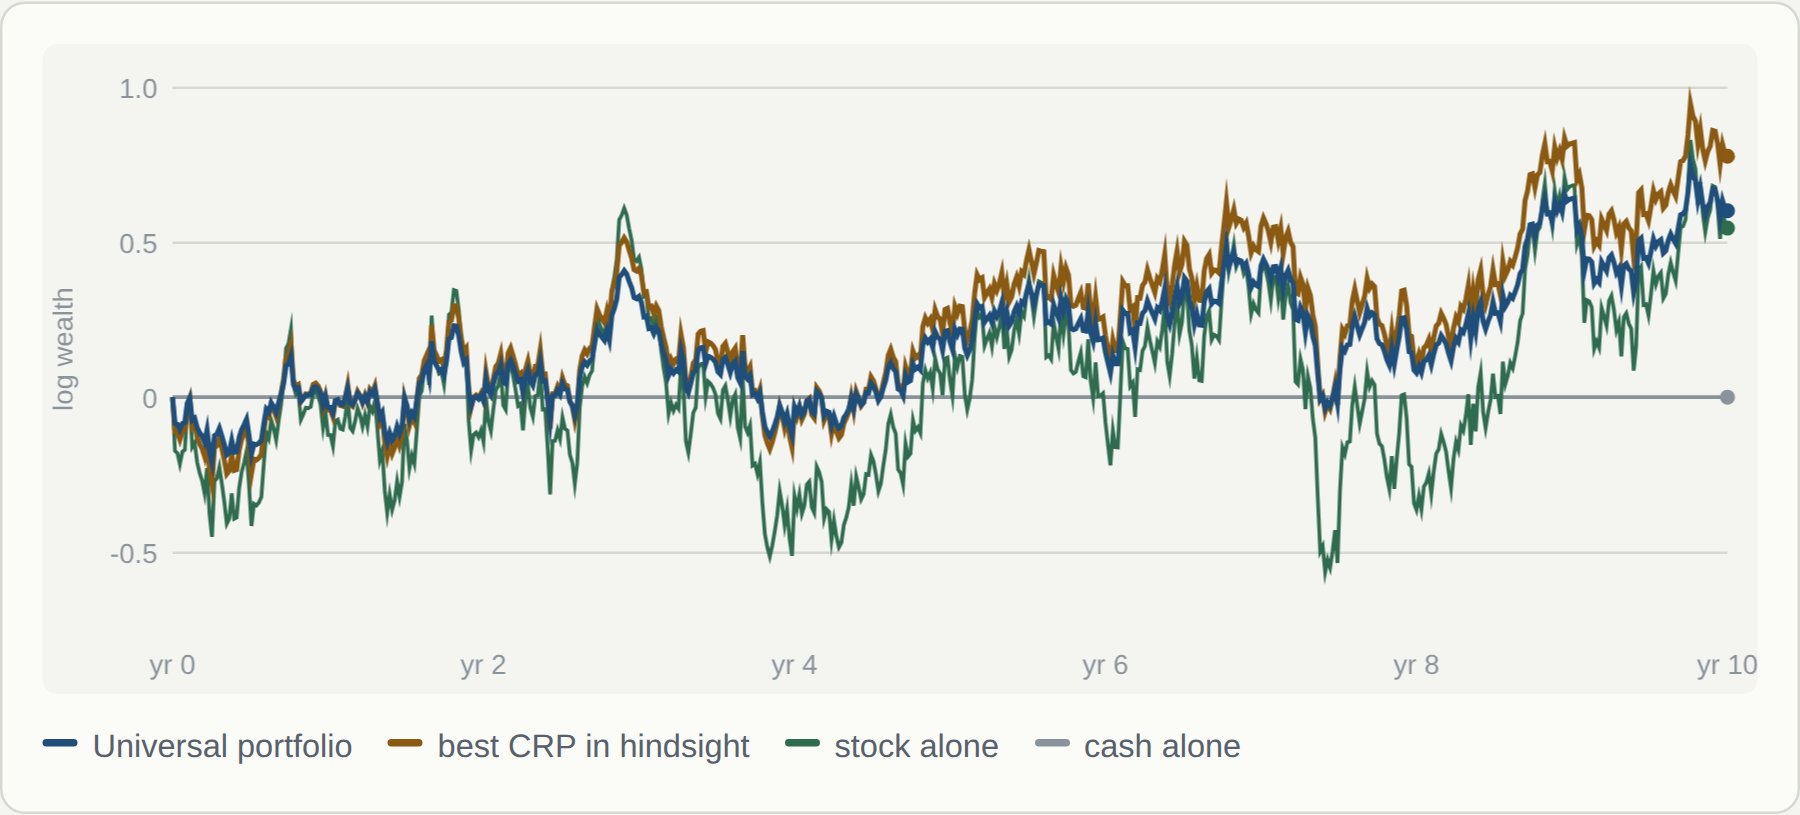
\includegraphics[width=\linewidth]{figures/demo-up}
\caption*{\small Two assets over ten years of daily data (2,520 days): cash, and a volatile stock whose log-price fluctuates around a trend with the chosen annual growth (it mean-reverts with a half-life of about four months). The universal portfolio is computed exactly by averaging all constant-rebalanced portfolios on a grid of 201 stock weights. With zero trend the stock ends roughly where it started, yet rebalanced portfolios grow steadily: that is volatility pumping, and the universal portfolio captures most of it without knowing the best mix. Press ``New market'' for other paths. \emph{(A static snapshot at the default settings; the HTML edition has live sliders.)}}
\end{figure}

\section*{11.4 Faster algorithms}\addcontentsline{toc}{section}{11.4 Faster algorithms}\label{ch11-fast}

\subsection*{Exponentiated gradient}

Helmbold, Schapire, Singer and Warmuth (1998) apply the entropic mirror step to the linearised loss. With gradient $\nabla f_t(x_t)=-r_t/\ip{x_t}{r_t}$ the update is

\[x_{t+1,i}\;\propto\;x_{t,i}\exp\Big(\eta\frac{r_{t,i}}{\ip{x_t}{r_t}}\Big).\]

It costs $O(n)$ per day. If all price relatives lie in $[c,C]$ with $c>0$, the gradients are bounded by $C/c$, and Theorem 10.4 gives regret $O\big(\frac Cc\sqrt{T\ln n}\big)$. The price for speed is a $\sqrt T$ rate and a dependence on how extreme the returns can be.

\subsection*{Exp-concavity and Online Newton Step}

\begin{bdef}{Definition 11.5 \emph{(exp-concave)}}
$f$ is $\alpha$-exp-concave if $e^{-\alpha f}$ is concave. The portfolio loss $f_t(x)=-\ln\ip{x}{r_t}$ is $1$-exp-concave, since $e^{-f_t}=\ip{x}{r_t}$ is linear.
\end{bdef}

Exp-concavity is weaker than strong convexity (it gives curvature only in the direction of the gradient) but it is enough for logarithmic regret. Online Newton Step (Hazan, Agarwal and Kale 2007) is OGD preconditioned by the running sum of gradient outer products $A_t=\eps I+\sum_{s\le t}g_sg_s^\top$:

\[x_{t+1}=\Pi^{A_t}_{\simplex_n}\big(x_t-\tfrac1\gamma A_t^{-1}g_t\big),\]

where the projection is in the norm $\norm{y}_{A_t}=\sqrt{y^\top A_ty}$. For $\alpha$-exp-concave losses with bounded gradients it has regret $O\big((\frac1\alpha+GD)\,n\ln T\big)$ at $O(n^2)$ cost per step, plus the projection. For portfolios it needs a lower bound on price relatives (or a mixing step with the uniform portfolio). Cover's theorem is thus one instance of a general principle: \emph{curvature buys logarithmic regret}.

\begin{center}\small
\begin{tabularx}{\linewidth}{YYYY}
\toprule
\textbf{Algorithm} & \textbf{Regret vs best CRP} & \textbf{Cost per day} & \textbf{Assumptions} \\
\midrule
Universal portfolio & $(n-1)\ln T+O(1)$ & integral over $\simplex_n$ & none \\
Exponentiated gradient & $O(\frac Cc\sqrt{T\ln n})$ & $O(n)$ & $r_{t,i}\in[c,C]$ \\
Online Newton Step & $O(n\ln T)$ up to constants & $O(n^2)$ plus projection & bounded gradients \\
\bottomrule
\end{tabularx}
\end{center}

\begin{bwarn}{Reality check}
The best CRP is a benchmark, not a strategy. Rebalancing daily into volatile, uncorrelated assets does pump volatility, but real markets have transaction costs, and the best CRP over real stock data is often concentrated in a few assets that happened to do well. Studies of these algorithms on historical data (e.g. Borodin, El-Yaniv and Gogan 2004; Li and Hoi 2014) find that the universal portfolio typically tracks a diversified CRP closely but rarely beats simple benchmarks after costs. The guarantee is about \emph{robustness}: you never do much worse than the best rebalancing rule, whatever happens.
\end{bwarn}

\begin{takeaways}
\begin{itemize}
\item Log-wealth is the right objective for repeated investment; the Kelly bet is $b^*=p$.
\item The best constant-rebalanced portfolio can beat every asset exponentially.
\item Cover's universal portfolio is EWA over all CRPs. Its regret $(n-1)\ln T+O(1)$ holds on every sequence with no parameters.
\item Exp-concavity of $-\ln\ip{x}{r}$ is the reason for logarithmic regret.
\end{itemize}
\end{takeaways}

\section*{Exercises}\addcontentsline{toc}{section}{Exercises}\label{ch11-ex}

\exercise{11.1}{\extag{fin}{finance}}{\hypertarget{sol-11.1}{}Three horses with win probabilities $(0.5,0.3,0.2)$ and odds $(1.8,3,6)$. (a) Is there an arbitrage? (b) Find the Kelly bet and its growth rate. (c) What is the growth rate of betting everything on the horse with the highest expected payoff?}

\exercise{11.2}{\extag{fin}{finance}}{\hypertarget{sol-11.2}{}Continuing 11.1, allow keeping a fraction $c$ in cash. Show that the optimal strategy bets only on horse 3, with fraction $f$ solving $\max_f\;0.2\ln(1-f+6f)+0.8\ln(1-f)$, and find $f$.}

\exercise{11.3}{\extag{med}{core}}{\hypertarget{sol-11.3}{}For Example 11.3, find the best CRP $x=(1-\theta,\theta)$ in hindsight and its growth per two days.}

\exercise{11.4}{\extag{med}{core}}{\hypertarget{sol-11.4}{}Show that $f(x)=-\ln\ip{x}{r}$ is convex but not strongly convex on $\simplex_n$, and verify that it is $1$-exp-concave.}

\exercise{11.5}{\extag{hard}{challenge}}{\hypertarget{sol-11.5}{}Show that the universal portfolio's wealth equals $\E_{x\sim\mathrm{Unif}(\simplex_n)}[W_T(x)]$, and use Laplace's method to argue that when the best CRP $x^*$ is interior and $\ln W_T(x)$ is strongly concave with curvature $\propto T$ near $x^*$, the regret is $\frac{n-1}2\ln T+O(1)$ rather than $(n-1)\ln T$.}

\subsection*{Solutions}
\begin{solutions}
\sol{11.1}{(a) $\sum1/o_i=0.556+0.333+0.167=1.056\ge1$, so no sure profit from betting on every horse. (b) $b^*=(0.5,0.3,0.2)$. Growth rate $=0.5\ln0.9+0.3\ln0.9+0.2\ln1.2=0.8\ln0.9+0.2\ln1.2=-0.0843+0.0365=-0.048$ per race. Negative: with these odds you should not bet at all if you may keep cash. (c) Expected payoffs $0.9,0.9,1.2$: all on horse 3 has growth rate $-\infty$ (bankruptcy with probability $0.8$ each race). Adding a cash option, the Kelly bet becomes a mix of cash and horse 3 only; finding it is Exercise 11.2.}
\sol{11.2}{Horses 1 and 2 have $p_io_i<1$, so money on them is better kept in cash. Betting $f$ on horse 3 multiplies wealth by $1+5f$ if it wins and $1-f$ otherwise. Setting the derivative to zero, $\frac{0.2\cdot5}{1+5f}=\frac{0.8}{1-f}$, so $1-f=0.8+4f$ and $f=0.04$. The Kelly fraction is $4\%$, matching the classic formula $f=\frac{p\,o-1}{o-1}=\frac{0.2}{5}$. The growth rate is $0.2\ln1.2+0.8\ln0.96\approx0.0038$ per race: small but positive.}
\sol{11.3}{Maximise $(1+\theta)(1-\theta/2)$: derivative $1-\theta/2-(1+\theta)/2=\frac12-\theta=0$, $\theta=\frac12$, growth factor $1.125$ per two days.}
\sol{11.4}{$\nabla^2f=\frac{rr^\top}{\ip{x}{r}^2}\succeq0$ has rank one, so it is flat in every direction orthogonal to $r$: convex, not strongly convex. $e^{-f}=\ip xr$ is linear, hence concave.}
\end{solutions}

\chapter[Probability as a game, options]{Probability as a Game, and Pricing Options}\label{ch12}
\chapsource{Based on Lecture 14 (Oct 23, 2013; with Rafael Frongillo) · \href{https://web.eecs.umich.edu/~jabernet/eecs598course/fall2013/web/notes/lec14_102313.pdf}{scribe notes} · Shafer and Vovk, \emph{Probability and Finance: It's Only a Game!} (2001), ch. 1}

\begin{goals}
\begin{itemize}
\item No-arbitrage pricing by replication on one- and two-period trees.
\item Shafer and Vovk's game-theoretic probability: upper and lower prices defined by hedging, with no probability measure.
\item A strong law of large numbers proved by a betting strategy, which turns out to be a universal portfolio.
\item Regret bounds as option-price bounds, and Black–Scholes as the value of a game.
\end{itemize}
\end{goals}

\begin{marginnote}
The dollar figures in the scribed examples for this lecture did not survive in the PDF. The numbers below are our own; they illustrate the same three phenomena (unique price, price interval, dynamic hedging restoring a unique price).
\end{marginnote}

\section*{12.1 Pricing by replication}\addcontentsline{toc}{section}{12.1 Pricing by replication}\label{ch12-trees}

Interest rates are zero throughout. A stock trades at $S_0=100$.

\begin{bexample}{Example 12.1 \emph{(one period, two outcomes)}}
Tomorrow $S_1\in\{80,120\}$. A call option struck at $100$ pays $(S_1-100)^+\in\{0,20\}$. Hold $\Delta$ shares and $c$ in cash, so tomorrow's value is $c+\Delta(S_1-100)$ (buying shares at $100$ costs nothing net if financed by borrowing). Matching both outcomes:

\[c+\Delta(80-100)=0,\qquad c+\Delta(120-100)=20\quad\Longrightarrow\quad\Delta=\tfrac12,\ c=10.\]

The option is worth exactly $10$. At a price of $12$ we would sell it, put $10$ into the replicating portfolio and pocket $2$ for sure; at $8$ we would do the reverse. The price $10$ is also $\E_q[(S_1-100)^+]$ under the unique ``risk-neutral'' $q$ with $\E_q[S_1]=S_0$, here $q=(\tfrac12,\tfrac12)$. The real-world probability of an up-move plays no role.
\end{bexample}

\begin{bexample}{Example 12.2 \emph{(one period, three outcomes)}}
Now $S_1\in\{80,100,120\}$ with payoff $(0,0,20)$. Three equations, two unknowns: no exact replication. The cheapest \emph{super-hedge} is the line through $(80,0)$ and $(120,20)$, which costs $10$ at $S=100$ and dominates the payoff at every outcome. The most expensive \emph{sub-hedge} is the line through $(80,0)$ and $(100,0)$, worth $0$. Any price in $[0,10]$ is arbitrage-free; outside it there is a sure profit. Probability-free reasoning gives an interval, not a number.
\end{bexample}

\begin{bexample}{Example 12.3 \emph{(two periods)}}
Split the day: by noon $S\in\{90,110\}$, by close each moves $\pm10$, reaching $\{80,100,120\}$ as before. Work backwards. At the $110$ node, outcomes $100\mapsto0$ and $120\mapsto20$ give $\Delta=1$ and value $10$. At the $90$ node both outcomes pay $0$: value $0$, $\Delta=0$. At the root, the ``payoffs'' are $0$ at $90$ and $10$ at $110$, so $\Delta=\tfrac12$ and the price is $5$. Trading at noon restores a unique price, inside the interval of Example 12.2. As trading becomes continuous, this binomial construction converges to Black–Scholes (Cox, Ross and Rubinstein 1979).
\end{bexample}

\begin{figure}[htbp]
\centering
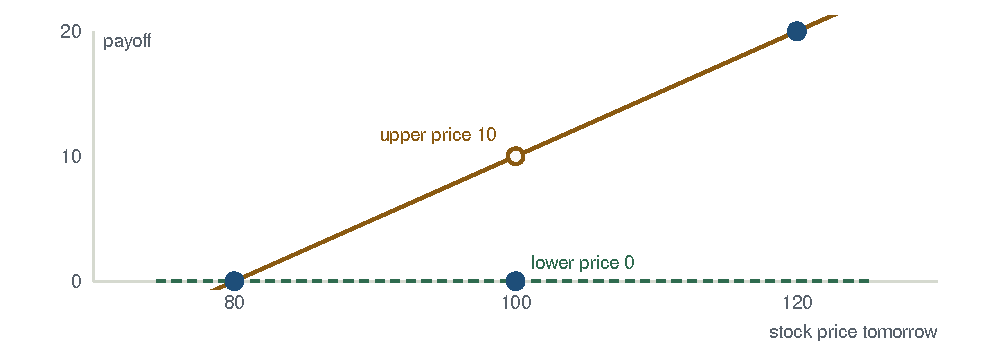
\includegraphics[width=\linewidth]{figures/ch12-fig1}
\caption*{\small Example 12.2 in pictures. Each hedge (cash plus $\Delta$ shares) is a line; its intercept at today's price is its cost. The upper price is the lowest line above all payoff points, the lower price the highest line below them. With two outcomes the points are always collinear and the two prices coincide.}
\end{figure}

\section*{12.2 Game-theoretic probability}\addcontentsline{toc}{section}{12.2 Game-theoretic probability}\label{ch12-sv}

Shafer and Vovk turn the picture above into a foundation for probability. There is no probability measure, only a game between two players.

\begin{bdef}{Definition 12.4 \emph{(the protocol)}}
\begin{itemize}
\item A tree of \emph{situations}. The root is $\square$; the move $\omega$ from situation $t$ leads to $t\omega$; leaves are terminal.
\item \textbf{World} chooses the moves. \textbf{Skeptic} chooses a strategy $P$, a bet $P(t)$ in each situation.
\item Skeptic's \emph{capital process} starts at $\mathcal K^P(\square)=0$ and changes linearly with World's move: $\mathcal K^P(t\omega)=\mathcal K^P(t)+P(t)\,\omega$. (In Example 12.1, $\omega=S_1-S_0$ and $P=\Delta$.)
\item A \emph{martingale} is $\alpha+\mathcal K^P$ for some initial capital $\alpha$ and strategy $P$.
\end{itemize}
\end{bdef}

\begin{bdef}{Definition 12.5 \emph{(upper and lower expectation)}}
For a payoff $x$ on terminal situations,

\[\begin{gathered}\overline{\E}[x]=\inf\{\alpha:\exists P\ \forall\text{ terminal }t,\ \alpha+\mathcal K^P(t)\ge x(t)\},\\
\underline{\E}[x]=\sup\{\alpha:\exists P\ \forall t,\ \alpha+\mathcal K^P(t)\le x(t)\}.\end{gathered}\]

When they agree, the common value is the (game-theoretic) expectation $\E[x]$. For an event $E$, the upper and lower probabilities are $\overline{\mathbb P}[E]=\overline\E[\ind_E]$ and $\underline{\mathbb P}[E]=\underline\E[\ind_E]$.
\end{bdef}

The upper expectation is the super-hedging price and the lower expectation the sub-hedging price. Written as

\[\overline\E[x]=\inf_P\ \sup_{t}\ \big(x(t)-\mathcal K^P(t)\big),\]

it is a minimax regret: Skeptic tries to track the payoff $x$ with trading gains, and $\overline\E[x]$ is the smallest worst-case shortfall. An event has upper probability zero if Skeptic can start with capital $1$, never go into debt, and become arbitrarily rich if the event happens. \emph{``Probability zero'' means ``you could get rich betting against it''.}

\section*{12.3 A strong law of large numbers by betting}\addcontentsline{toc}{section}{12.3 A strong law of large numbers by betting}\label{ch12-slln}

\begin{bthm}{Theorem 12.6 \emph{(game-theoretic SLLN, Shafer and Vovk 2001)}}
In the protocol where, at each round $i=1,2,\dots$, Skeptic bets $P_i$ and then World picks $\omega_i\in[-1,1]$, Skeptic has a strategy that starts with capital $1$, never goes negative, and whose capital is unbounded on every path where $\frac1n\sum_{i\le n}\omega_i\not\to0$. In other words, $\overline{\mathbb P}\big[\tfrac1n\sum_i\omega_i\not\to0\big]=0$.
\end{bthm}

\begin{proof}
\emph{One bettor.} Bet the fraction $\eps\in[-\tfrac12,\tfrac12]$ of current capital each round, so capital after $n$ rounds is $K^\eps_n=\prod_{i\le n}(1+\eps\omega_i)>0$. Since $\ln(1+x)\ge x-x^2$ for $\abs x\le\frac12$,

\[\ln K^\eps_n\;\ge\;\eps S_n-\eps^2n,\qquad S_n=\sum_{i\le n}\omega_i.\]

\emph{Many bettors.} Split initial capital: weight $2^{-k-1}$ each to the bettors with $\eps=+2^{-k}$ and $\eps=-2^{-k}$, $k=1,2,\dots$. Each account stays positive, so total capital $K_n\ge2^{-k-1}K_n^{\pm2^{-k}}$ for every $k$.

\emph{Conclusion.} If $\limsup S_n/n>\delta>0$, pick $k$ with $2^{-k}<\delta/2$. Along the subsequence where $S_n>\delta n$, $\ln K_n^{2^{-k}}\ge n\,2^{-k}(\delta-2^{-k})\to\infty$, so $K_n$ is unbounded. The case $\liminf S_n/n<0$ uses the negative bettors.
\end{proof}

Look at the structure of that proof: a mixture of constant-fraction betting strategies, with fixed prior weights, compared to the best of them in hindsight, in log-wealth. It is exactly the argument behind Cover's universal portfolio (Chapter 11) and EWA with a prior (Theorem 3.9). The law of large numbers, seen from the game-theoretic side, \emph{is} a no-regret statement: a universal bettor gets rich whenever any simple bettor does, so if the averages do not converge, some simple bettor, and hence the universal one, gets rich.

\section*{12.4 Regret bounds are option-price bounds}\addcontentsline{toc}{section}{12.4 Regret bounds are option-price bounds}\label{ch12-options}

Reverse the roles. Suppose an online algorithm trading a stock and cash, starting with capital $1$, guarantees on every price path in some class $\mathcal S$ that its final wealth is at least $\beta\max\big(S_T/S_0,\,1\big)$ for some $\beta\in(0,1]$. This is a multiplicative no-regret guarantee against the two ``experts'' hold-the-stock and hold-cash. Consider the claim that pays $\max(S_T/S_0,1)$, and suppose it is priced above $1/\beta$. Sell it, run the algorithm with capital $1/\beta$, and keep the difference: at maturity the algorithm's wealth covers the payoff on every path in $\mathcal S$. So, with no probability model,

\[\begin{gathered}\text{price}\big[\max(S_T/S_0,1)\big]\;\le\;\frac1\beta,\\
\text{and since}\quad \frac{(S_T-S_0)^+}{S_0}=\max\Big(\frac{S_T}{S_0},1\Big)-1,\quad \frac{\text{call}_{K=S_0}}{S_0}\le\frac1\beta-1.\end{gathered}\]

DeMarzo, Kremer and Mansour (2006) made this precise. Take $\mathcal S$ to be paths whose quadratic variation $\sum_t(\ln S_{t+1}-\ln S_t)^2$ is at most $Q$, the path-wise analogue of $\sigma^2T$. A Hedge-type algorithm over the two assets has log-wealth regret of order $\sqrt Q$, so $\beta=e^{-O(\sqrt Q)}$ and the at-the-money call is worth at most $S_0\big(e^{O(\sqrt Q)}-1\big)\approx O(\sqrt Q)\,S_0$. Compare Black–Scholes: the at-the-money call is worth about $0.4\,S_0\,\sigma\sqrt T=0.4\,S_0\sqrt Q$. The $\sqrt T$ of regret and the $\sigma\sqrt T$ of option prices are the same phenomenon.

The lecture's co-instructor Rafael Frongillo, with Abernethy and others, took this to its conclusion (Abernethy, Frongillo and Wibisono 2012; Abernethy, Bartlett, Frongillo and Wibisono 2013). Define the minimax price of an option as the value of a hedging game in which Nature moves the price subject to a quadratic-variation budget and a bound on each jump, and the Investor hedges. As the jump bound tends to zero, the value of this game converges to the Black–Scholes price. Black–Scholes then needs no Brownian motion: it is the price of a game against an adversary with a volatility budget.

\begin{bfin}{Why this matters in practice}
\begin{itemize}
\item Model-free bounds (super- and sub-hedging prices) are what a trader can defend when they do not trust a model. Examples 12.2 and 12.3 show they can be wide or tight depending on what is tradeable.
\item The volatility budget $Q$ plays the role of implied volatility. Robust hedging strategies driven by realised quadratic variation, such as variance swaps and ``hedging with a volatility band'', are practical relatives of these ideas.
\item No-regret algorithms, read backwards, are hedging strategies. Every regret bound in this book has a financial meaning as the capital needed to super-replicate some payoff.
\end{itemize}
\end{bfin}

\begin{takeaways}
\begin{itemize}
\item Replication gives unique prices when the market is complete, and a price interval otherwise.
\item Upper and lower expectations are super- and sub-hedging prices, i.e. minimax regret problems for Skeptic.
\item The strong law of large numbers is a universal-portfolio argument.
\item Regret bounds give option-price upper bounds; with a quadratic-variation budget the game's value tends to Black–Scholes.
\end{itemize}
\end{takeaways}

\section*{Exercises}\addcontentsline{toc}{section}{Exercises}\label{ch12-ex}

\exercise{12.1}{\extag{fin}{finance}}{\hypertarget{sol-12.1}{}In Example 12.1, price a put struck at $100$ by replication, and verify put–call parity $C-P=S_0-K$.}

\exercise{12.2}{\extag{fin}{finance}}{\hypertarget{sol-12.2}{}In Example 12.2, find all risk-neutral measures $q$ on $\{80,100,120\}$ (with $\E_qS_1=100$) and show that $\{\E_q[\text{payoff}]\}$ is exactly $[0,10]$ (open or closed, depending on whether $q$ must be strictly positive).}

\exercise{12.3}{\extag{med}{core}}{\hypertarget{sol-12.3}{}Show the martingale property: in a one-step game where the lower and upper expectation of World's move $\omega$ are both $0$, every capital process $s=\alpha+\mathcal K^P$ satisfies $\E[s(t\omega)\mid t]=s(t)$.}

\exercise{12.4}{\extag{hard}{challenge}}{\hypertarget{sol-12.4}{}Using Hedge with $N=2$ experts (``stock'' and ``cash'') on log-returns bounded by $\delta$ per step, derive a bound of the form $\ln W_T\ge\max(\ln S_T/S_0,0)-c\sqrt{Q\ln2}-O(\delta)$ and deduce an explicit upper bound on the at-the-money call price in terms of $Q$.}

\subsection*{Solutions}
\begin{solutions}
\sol{12.1}{Put payoff $(20,0)$: $\Delta=-\frac12$, $c=0-(-\tfrac12)(120-100)=10$. So $P=10$, and $C-P=0=S_0-K$.}
\sol{12.2}{$q=(a,1-2a,a)$ for $a\in[0,\tfrac12]$. $\E_q[\text{payoff}]=20a\in[0,10]$. With strictly positive $q$, $a\in(0,\tfrac12)$ and the set is $(0,10)$. This is the duality between super-hedging and risk-neutral pricing (LP duality again).}
\sol{12.3}{$s(t\omega)=s(t)+P(t)\omega$ is affine in $\omega$ with slope $P(t)$. Super-hedge it with initial capital $s(t)$ and bet $P(t)$; sub-hedge it the same way. Both prices equal $s(t)$.}
\end{solutions}

\def\thepartblurb{Learning when you only see the outcome of what you chose.}\part{Bandits}\label{part5}

\chapter[Stochastic bandits]{Stochastic Bandits: Explore, Exploit, Be Optimistic}\label{ch13}
\chapsource{Based on Lectures 18–19 (Nov 6 and 11, 2013) · \href{https://web.eecs.umich.edu/~jabernet/eecs598course/fall2013/web/notes/lec18_110613.pdf}{notes 18} · \href{https://web.eecs.umich.edu/~jabernet/eecs598course/fall2013/web/notes/lec19_111113.pdf}{notes 19}}

\begin{goals}
\begin{itemize}
\item The bandit feedback model and pseudo-regret.
\item Explore-then-commit and its $O(N\ln(NT)/\Delta^2)$ regret.
\item UCB: optimism in the face of uncertainty, $O(\sum_j\ln T/\Delta_j)$ regret.
\end{itemize}
\end{goals}

\section*{13.1 Bandit feedback}\addcontentsline{toc}{section}{13.1 Bandit feedback}\label{ch13-setting}

So far the learner saw the loss of every expert each round. In many problems it sees only the loss of the action it took: the fill price of the venue it routed to, the click-through of the ad it showed, the return of the strategy it funded. This is the \emph{multi-armed bandit} problem, named after slot machines (``one-armed bandits'').

\begin{bdef}{Protocol 13.1 \emph{(bandit)}}
$N$ arms. On round $t$ each arm has a loss $X_{i,t}\in[0,1]$. The learner picks $I_t$ (possibly at random) and observes and pays \emph{only} $X_{I_t,t}$. In the \textbf{stochastic} setting, $X_{i,t}$ are i.i.d. over $t$ with mean $\mu_i$; in the \textbf{adversarial} setting (Chapter 14) they are arbitrary. With $i^*=\argmin_i\mu_i$ and gaps $\Delta_j=\mu_j-\mu_{i^*}$, the (pseudo-)regret is

\[\bar R_T=\E\sum_{t=1}^T\big(\mu_{I_t}-\mu_{i^*}\big)=\sum_{j\neq i^*}\Delta_j\,\E[T_j(T)],\]

where $T_j(t)$ is the number of times arm $j$ was played in the first $t$ rounds.
\end{bdef}

The last identity is the key to every analysis in this chapter: regret is controlled by how often we pull each suboptimal arm. The tension is between \emph{exploration} (pull uncertain arms to learn about them) and \emph{exploitation} (pull the arm that looks best).

\begin{bthm}{Lemma 13.2 \emph{(Hoeffding's inequality)}}
If $Z_1,\dots,Z_m$ are i.i.d. in $[0,1]$ with mean $\mu$, then $\Pr\big[\abs{\tfrac1m\sum_jZ_j-\mu}\ge\eps\big]\le2e^{-2m\eps^2}$, and each one-sided deviation has probability at most $e^{-2m\eps^2}$. (Proof in \hyperref[appA]{Appendix A}.)
\end{bthm}

\section*{13.2 Explore then commit}\addcontentsline{toc}{section}{13.2 Explore then commit}\label{ch13-etc}

\begin{balg}{Algorithm 13.3 \emph{(explore-then-commit, ETC)}}
\begin{algo}
input: m \ensuremath{\ge} 1
for each arm i: play it m times, let \ensuremath{\hat{\mu}}\_i be its average loss   \# t = 1..Nm
for t > Nm: play \ensuremath{\hat\imath} = argmin\_i \ensuremath{\hat{\mu}}\_i
\end{algo}
\end{balg}

\begin{bthm}{Theorem 13.4}
If every suboptimal arm has gap at least $\Delta>0$, ETC with $m=\big\lceil\frac2{\Delta^2}\ln(2NT)\big\rceil$ has $\bar R_T\le1+Nm\le 1+N+\frac{2N\ln(2NT)}{\Delta^2}$.
\end{bthm}

\begin{proof}
Exploration costs at most $Nm$ since losses are in $[0,1]$. If ETC commits to a wrong arm $j$, then $\hat\mu_j\le\hat\mu_{i^*}$, so $\Delta\le\mu_j-\mu_{i^*}\le(\mu_j-\hat\mu_j)+(\hat\mu_{i^*}-\mu_{i^*})\le2\max_i\abs{\hat\mu_i-\mu_i}$. By Hoeffding and a union bound, $\Pr[\text{wrong commit}]\le2Ne^{-m\Delta^2/2}\le\frac1T$ for our $m$. The exploitation phase then costs at most $T\cdot\frac1T=1$ in expectation.
\end{proof}

ETC has two weaknesses. It needs to know $\Delta$ (or $T$) to set $m$, and it spends the same effort on an arm that is obviously bad after two pulls as on one that is hard to distinguish from the best. The $1/\Delta^2$ dependence is the price: without knowing $\Delta$, tuning for the worst case gives $O(T^{2/3})$ regret (Exercise 13.2).

\section*{13.3 Upper confidence bounds}\addcontentsline{toc}{section}{13.3 Upper confidence bounds}\label{ch13-ucb}

UCB resolves the tension with one principle: \emph{act as if the world is as favourable as is plausible given the data}. For losses, ``favourable'' means the lowest plausible mean. An arm is played either because its estimate is good (exploitation) or because it is uncertain (exploration), and uncertainty shrinks with every pull.

\begin{balg}{Algorithm 13.5 \emph{(UCB1, Auer, Cesa-Bianchi and Fischer 2002; loss form)}}
\begin{algo}
play each arm once
for t = N+1, …, T:
    I\_t \ensuremath{\leftarrow} argmin\_j  [ \ensuremath{\hat{\mu}}\_j \ensuremath{-} sqrt( 2 ln t / T\_j(t\ensuremath{-}1) ) ]
\end{algo}

The bonus $\sqrt{2\ln t/T_j}$ is the width of a Hoeffding confidence interval at confidence level $1-t^{-4}$.
\end{balg}

\begin{bthm}{Theorem 13.6}
For every suboptimal arm $j$, $\;\E[T_j(T)]\le\frac{8\ln T}{\Delta_j^2}+1+\frac{\pi^2}3$. Hence

\[\bar R_T\;\le\;\sum_{j:\Delta_j>0}\Big(\frac{8\ln T}{\Delta_j}+\big(1+\tfrac{\pi^2}{3}\big)\Delta_j\Big).\]

\end{bthm}

\begin{proof}
Write $c_{t,s}=\sqrt{2\ln t/s}$ and let $\ell=\lceil8\ln T/\Delta_j^2\rceil$. If arm $j$ is chosen at round $t$ after it has already been pulled $s\ge\ell$ times, while the optimal arm has been pulled $s^*$ times, then $\hat\mu_{j,s}-c_{t,s}\le\hat\mu_{*,s^*}-c_{t,s^*}$. At least one of three things must then hold:

\begin{enumerate}
\item $\hat\mu_{*,s^*}-c_{t,s^*}>\mu_*$: the optimal arm's lower confidence bound is too high;
\item $\hat\mu_{j,s}+c_{t,s}<\mu_j$: arm $j$'s estimate is too low;
\item $\mu_j-2c_{t,s}<\mu_*$, i.e. $\Delta_j<2c_{t,s}$.
\end{enumerate}

(If none holds, $\hat\mu_{j,s}-c_{t,s}\ge\mu_j-2c_{t,s}\ge\mu_*\ge\hat\mu_{*,s^*}-c_{t,s^*}$, and ties aside $j$ is not chosen.) Event 3 is impossible when $s\ge\ell$, because then $2c_{t,s}\le2\sqrt{2\ln T/\ell}\le\Delta_j$. By Hoeffding, events 1 and 2 each have probability at most $e^{-2s\cdot2\ln t/s}=t^{-4}$ for fixed $s,s^*$. So

\[\E[T_j(T)]\le\ell+\sum_{t=1}^\infty\sum_{s=1}^{t}\sum_{s^*=1}^{t}2t^{-4}\le\ell+\sum_{t\ge1}2t^{-2}=\ell+\frac{\pi^2}3.\]

\end{proof}

Compare with ETC: the dependence on each gap is $1/\Delta_j$ rather than $1/\Delta^2$, no parameters need tuning, and each arm's exploration adapts to its own gap. Taking the worst case over gaps gives a distribution-free bound of $O(\sqrt{NT\ln T})$ (Exercise 13.3).

\begin{bthm}{Theorem 13.7 \emph{(Lai and Robbins 1985, informal)}}
For any algorithm that has $o(T^a)$ regret on every instance for every $a>0$, and Bernoulli arms,

\[\liminf_{T\to\infty}\frac{\E[T_j(T)]}{\ln T}\;\ge\;\frac{1}{\KL(\mu_j\,\|\,\mu^*)}\quad\text{for each suboptimal }j,\]

where $\KL$ is between Bernoulli distributions. Since $\KL(\mu_j\|\mu^*)\le\frac{\Delta_j^2}{\mu^*(1-\mu^*)}$, this shows UCB's $\ln T/\Delta_j$ per-arm regret is optimal up to constants. Refinements such as KL-UCB and Thompson sampling achieve the exact constant.
\end{bthm}

\begin{bfin}{In finance}
Order routing is a natural stochastic bandit. A broker splits child orders across $N$ venues or algorithms, and observes the implementation shortfall only for the venue actually used. UCB routes most flow to the venue with the best observed shortfall while guaranteeing that every venue is re-tested at a rate of order $\ln t$, so a venue whose quality improves is eventually noticed. Two caveats from the theory apply. First, the i.i.d. assumption is doubtful: venue quality depends on market conditions and on your own flow. Second, regret $\sum_j\ln T/\Delta_j$ blows up when venues are nearly identical, which is also when choosing among them matters least. When the environment may be adversarial (other traders learning about your routing), use the methods of Chapter 14.
\end{bfin}

\begin{takeaways}
\begin{itemize}
\item Bandit regret equals $\sum_j\Delta_j\E[T_j(T)]$: control how often bad arms are pulled.
\item Explore-then-commit: $O(N\ln(NT)/\Delta^2)$, but needs the gap.
\item UCB: optimism gives $O(\sum_j\ln T/\Delta_j)$, matching the Lai–Robbins lower bound up to constants.
\end{itemize}
\end{takeaways}

\section*{Exercises}\addcontentsline{toc}{section}{Exercises}\label{ch13-ex}

\exercise{13.1}{\extag{easy}{warm-up}}{\hypertarget{sol-13.1}{}With $N=5$, $\Delta=0.05$ and $T=10^6$, compute the exploration length of ETC from Theorem 13.4 and compare with UCB's bound on $\E[T_j(T)]$ for an arm with gap $0.05$.}

\exercise{13.2}{\extag{med}{core}}{\hypertarget{sol-13.2}{}Show that ETC with $m$ chosen without knowledge of $\Delta$ can guarantee $\bar R_T=O(T^{2/3}(N\ln T)^{1/3})$. Hint: an arm with gap below $\eps$ costs at most $\eps T$ even if chosen.}

\exercise{13.3}{\extag{med}{core}}{\hypertarget{sol-13.3}{}Derive UCB's distribution-free bound $\bar R_T=O(\sqrt{NT\ln T})$. Hint: split arms into those with $\Delta_j<\delta$ and the rest.}

\exercise{13.4}{\extag{hard}{project}}{\hypertarget{sol-13.4}{}Simulate ETC, $\eps$-greedy, UCB1 and Thompson sampling (Beta–Bernoulli) on 10 Bernoulli arms with means spaced $0.02$ apart. Plot regret against $\ln T$. Which slopes match Theorems 13.6 and 13.7?}

\subsection*{Solutions}
\begin{solutions}
\sol{13.1}{ETC: $m=\lceil\frac{2}{0.0025}\ln(10^7)\rceil=\lceil800\times16.118\rceil=12{,}895$ pulls of each arm, total $64{,}475$. UCB: $\frac{8\ln10^6}{0.0025}\approx44{,}210$ pulls for that arm, plus a constant. The constants in UCB's analysis are loose; in practice it pulls such an arm far fewer times.}
\sol{13.2}{With $m$ pulls per arm, all estimates are within $\sqrt{\ln(2NT)/(2m)}$ w.h.p., so the committed arm has gap at most $2\sqrt{\ln(2NT)/(2m)}$. Regret $\le Nm+T\sqrt{2\ln(2NT)/m}+1$. Balancing gives $m\approx(T/N)^{2/3}(\ln(NT))^{1/3}$ and regret $O(N^{1/3}T^{2/3}(\ln NT)^{1/3})$.}
\sol{13.3}{Arms with $\Delta_j<\delta$ contribute at most $\delta T$. The rest contribute at most $\sum_j\frac{8\ln T}{\Delta_j}+O(N)\le\frac{8N\ln T}{\delta}+O(N)$. Set $\delta=\sqrt{8N\ln T/T}$.}
\end{solutions}

\chapter[Adversarial bandits]{Adversarial Bandits: EXP3 and Beyond}\label{ch14}
\chapsource{Based on Lectures 19–21 (Nov 11 – 18, 2013) · \href{https://web.eecs.umich.edu/~jabernet/eecs598course/fall2013/web/notes/lec20_111313.pdf}{notes 20} · \href{https://web.eecs.umich.edu/~jabernet/eecs598course/fall2013/web/notes/lec21_111813.pdf}{notes 21}}

\begin{goals}
\begin{itemize}
\item Importance-weighted loss estimates and why they are enough.
\item From $T^{3/4}$ to $T^{2/3}$ to $\sqrt T$: $\eps$-exploration versus EXP3.
\item The $\Omega(\sqrt{NT})$ lower bound, and bandits over combinatorial and convex sets.
\end{itemize}
\end{goals}

\section*{14.1 Estimating what you did not see}\addcontentsline{toc}{section}{14.1 Estimating what you did not see}\label{ch14-est}

With adversarial losses, a deterministic learner is hopeless: the adversary puts loss $1$ on whatever arm it will pick and $0$ elsewhere. So the learner must randomise, picking $I_t\sim p_t$. It then sees one coordinate of $\ell_t$ and needs a stand-in for the rest.

\begin{bdef}{Definition 14.1 \emph{(importance-weighted estimator)}}

\[\tilde\ell_{t,i}=\frac{\ell_{t,I_t}}{p_{t,I_t}}\ind[I_t=i].\]

It is unbiased: $\E_{I_t\sim p_t}\tilde\ell_{t,i}=p_{t,i}\cdot\frac{\ell_{t,i}}{p_{t,i}}=\ell_{t,i}$.
\end{bdef}

\begin{bthm}{Lemma 14.2 \emph{(unbiased estimates suffice)}}
Let $\mathcal F_{t-1}$ be the history before round $t$. If $p_t$ is $\mathcal F_{t-1}$-measurable and $\E[\tilde\ell_t\mid\mathcal F_{t-1}]=\ell_t$, then for any fixed $u\in\simplex_N$ (oblivious adversary), $\E\sum_t\ip{\tilde\ell_t}{p_t-u}=\E\sum_t\ip{\ell_t}{p_t-u}$.
\end{bthm}

So any full-information algorithm run on the estimates inherits its regret bound in expectation, \emph{except} that the bounds of Part I assumed losses in $[0,1]$, while $\tilde\ell_{t,i}$ can be as large as $1/p_{t,i}$. The whole difficulty of adversarial bandits is controlling the size of these estimates.

\section*{14.2 A first attempt: separate exploration}\addcontentsline{toc}{section}{14.2 A first attempt: separate exploration}\label{ch14-eps}

With probability $\eps$, explore: play a uniformly random arm and set $\tilde\ell_t=\frac{N}{\eps}\ell_{t,I_t}e_{I_t}$. Otherwise exploit: play Hedge on past estimates and set $\tilde\ell_t=0$. The estimate is unbiased and bounded by $N/\eps$. Plugging this range into the Hedge bound gives regret $O\big(\eps T+\frac{\ln N}\eta+\eta T\frac{N^2}{\eps^2}\big)=O\big(T^{3/4}\sqrt N(\ln N)^{1/4}\big)$. A finer analysis uses the second-moment term $\sum_ip_{t,i}\tilde\ell_{t,i}^2$ that appears in the proof of Theorem 14.4 below; its expectation here is at most $\eps\cdot\frac1N\sum_ip_{t,i}\frac{N^2}{\eps^2}\le\frac N\eps$. That gives $O\big(\eps T+\frac{\ln N}\eta+\frac{\eta TN}{\eps}\big)=O\big(T^{2/3}(N\ln N)^{1/3}\big)$. Both are worse than $\sqrt T$ because exploration rounds are wasted: they pay loss without exploiting, and exploiting rounds teach nothing.

\section*{14.3 EXP3}\addcontentsline{toc}{section}{14.3 EXP3}\label{ch14-exp3}

\begin{balg}{Algorithm 14.3 \emph{(EXP3, Auer, Cesa-Bianchi, Freund and Schapire 2002)}}
\begin{algo}
input: \ensuremath{\eta} > 0;  \ensuremath{\tilde{L}}\_\{i,0\} \ensuremath{\leftarrow} 0
for t = 1, …, T:
    p\_\{t,i\} \ensuremath{\leftarrow} exp(\ensuremath{-}\ensuremath{\eta} \ensuremath{\tilde{L}}\_\{i,t\ensuremath{-}1\}) / \ensuremath{\Sigma}\_j exp(\ensuremath{-}\ensuremath{\eta} \ensuremath{\tilde{L}}\_\{j,t\ensuremath{-}1\})
    draw I\_t \ensuremath{\sim} p\_t;  observe \ensuremath{\ell}\_\{t,I\_t\}
    \ensuremath{\tilde{L}}\_\{I\_t,t\} \ensuremath{\leftarrow} \ensuremath{\tilde{L}}\_\{I\_t,t\ensuremath{-}1\} + \ensuremath{\ell}\_\{t,I\_t\} / p\_\{t,I\_t\}      \# other arms unchanged
\end{algo}

EXP3 = ``exponential weights for exploration and exploitation''. Every round both exploits and gathers information.
\end{balg}

\begin{bthm}{Theorem 14.4}
Against an oblivious adversary with losses in $[0,1]$, EXP3 satisfies $\E\,\Reg_T\le\frac{\ln N}{\eta}+\frac{\eta NT}{2}$. With $\eta=\sqrt{\frac{2\ln N}{NT}}$, $\;\E\,\Reg_T\le\sqrt{2NT\ln N}$.
\end{bthm}

\begin{proof}
Use the softmin potential $\Phi_t=-\frac1\eta\ln\sum_ie^{-\eta\tilde L_{i,t-1}}$. As in Chapter 3,

\[\Phi_{t+1}-\Phi_t=-\frac1\eta\ln\E_{i\sim p_t}e^{-\eta\tilde\ell_{t,i}}.\]

Because estimates are nonnegative we can use $e^{-x}\le1-x+\frac{x^2}2$ for $x\ge0$, then $-\ln(1-y)\ge y$:

\[\Phi_{t+1}-\Phi_t\;\ge\;\sum_ip_{t,i}\tilde\ell_{t,i}-\frac\eta2\sum_ip_{t,i}\tilde\ell_{t,i}^2.\]

This is the step that avoids needing $\tilde\ell\le1$: only nonnegativity is used, and the price is a \emph{second-moment} term. Now take expectations over $I_t$:

\[\begin{gathered}\E\sum_ip_{t,i}\tilde\ell_{t,i}=\ip{p_t}{\ell_t},\\
\E\sum_ip_{t,i}\tilde\ell_{t,i}^2=\sum_ip_{t,i}\cdot p_{t,i}\frac{\ell_{t,i}^2}{p_{t,i}^2}=\sum_i\ell_{t,i}^2\le N.\end{gathered}\]

The $1/p$ blow-up is exactly cancelled by weighting with $p$. Summing over $t$, $\E[\Phi_{T+1}-\Phi_1]\ge\E\sum_t\ip{p_t}{\ell_t}-\frac{\eta NT}2$. On the other side, $\Phi_1=-\frac{\ln N}\eta$ and $\Phi_{T+1}\le\tilde L_{u,T}$ for any arm $u$, with $\E\tilde L_{u,T}=L_{u,T}$. Rearrange.
\end{proof}

The comparison with full information is instructive: Hedge's regret is $\sqrt{(T/2)\ln N}$; EXP3 pays an extra $\sqrt N$, the price of seeing one coordinate out of $N$. That price is unavoidable.

\begin{bthm}{Theorem 14.5 \emph{(lower bound; Auer et al. 2002; Homework 3)}}
For every algorithm there is a stochastic instance with $\bar R_T\ge c\sqrt{NT}$ for a universal constant $c>0$.
\end{bthm}

\begin{proof}[Idea]
All arms are fair coins (loss $\tfrac12$ in expectation) except a secret arm with mean $\tfrac12-\eps$. Identifying a biased coin among $N$ requires about $N/\eps^2$ flips in total, because each arm needs about $1/\eps^2$ samples to be distinguished from fair (the KL divergence per sample is $\Theta(\eps^2)$). An algorithm with regret $\ll\eps T$ must play the secret arm most of the time, so it effectively identifies it, which is impossible if $T\ll N/\eps^2$. Setting $\eps=\sqrt{N/T}$ gives regret $\Omega(\eps T)=\Omega(\sqrt{NT})$.
\end{proof}

Refinements: the $\sqrt{\ln N}$ gap between the bounds is closed by the INF algorithm (Audibert and Bubeck 2009), which is FTRL with the regularizer $-\sum_i\sqrt{x_i}$. EXP3's regret holds only in expectation; its variance is large, and EXP3.P adds explicit exploration to get high-probability bounds.

\section*{14.4 Bandits on combinatorial and convex sets}\addcontentsline{toc}{section}{14.4 Bandits on combinatorial and convex sets}\label{ch14-linear}

Suppose each round we choose an $s$–$t$ path in a graph with $d$ edges and pay the sum of edge delays, observing only the total delay of our path. Paths are exponentially many, so EXP3 over paths has regret $\sqrt{2(\#\text{paths})\,T\ln(\#\text{paths})}$, which is useless. The fix is to work in the convex hull of path indicator vectors (the flow polytope $\cK\subset\R^d$) with linear losses $\ip{f_t}{x}$, and run FTRL on estimated loss vectors:

\[x_t=\argmin_{x\in\cK}\ \sum_{s<t}\ip{\tilde f_s}{x}+\frac1\eta R(x),\quad\text{then play a random path }y_t\text{ with }\E y_t=x_t.\]

Since regret is linear in the losses for a fixed comparator, unbiased estimates again suffice in expectation. The problem is again the size of $\tilde f_t$: near the boundary of $\cK$ we must divide by small numbers.

Abernethy, Hazan and Rakhlin (2008) solved this by choosing $R$ to be a \textbf{self-concordant barrier} for $\cK$ (for a polytope $\{x:a_k^\top x\le b_k\}$, the log-barrier $-\sum_k\ln(b_k-a_k^\top x)$) and measuring everything in the local norm $\norm{v}_{x}=\sqrt{v^\top\nabla^2R(x)v}$. The key geometric fact is that the Dikin ellipsoid $\{y:\norm{y-x}_x\le1\}$ lies inside $\cK$. Their algorithm, SCRiBLe, plays a random endpoint of one of the ellipsoid's principal axes, $y_t=x_t\pm\lambda_i^{-1/2}e_i$ (where $\lambda_i,e_i$ are eigenpairs of $\nabla^2R(x_t)$), and sets $\tilde f_t=d\,\ip{f_t}{y_t}\,\xi_t\lambda_i^{1/2}e_i$ with $\xi_t=\pm1$ the chosen sign. This estimate is unbiased and has local dual norm at most $d$, and the result is

\[\E\,\Reg_T=O\big(d\sqrt{\theta\,T\ln T}\big),\]

where $\theta$ is the barrier's self-concordance parameter ($\theta=m$ for the log-barrier of $m$ constraints). This was the first efficient $\sqrt T$ algorithm for bandit linear optimization.

\begin{bfin}{In finance}
Adversarial bandits suit trading problems where your own actions change the environment, or where competitors adapt. Examples include choosing which of $N$ execution algorithms to use for each parent order (other participants may detect and front-run a predictable choice), or setting quotes as a market maker (you observe only whether your quote was hit, not what would have happened at other prices). EXP3 guarantees average performance within $\sqrt{2N\ln N/T}$ per round of the best fixed choice, against any behaviour of the other side, provided that behaviour does not react to your internal random draws. The randomisation is a feature: an unpredictable router is harder to exploit.
\end{bfin}

\begin{takeaways}
\begin{itemize}
\item Importance weighting $\tilde\ell_{t,i}=\ell_{t,I_t}\ind[I_t=i]/p_{t,i}$ gives unbiased estimates; regret bounds transfer in expectation.
\item EXP3 is Hedge on these estimates. The second moment $\sum_ip_{t,i}\tilde\ell_{t,i}^2$ has expectation at most $N$, giving $\sqrt{2NT\ln N}$.
\item $\Omega(\sqrt{NT})$ is unavoidable: bandit feedback costs a factor $\sqrt N$.
\item For structured action sets, FTRL with a self-concordant barrier and ellipsoid sampling gives $O(d\sqrt{\theta T\ln T})$.
\end{itemize}
\end{takeaways}

\section*{Exercises}\addcontentsline{toc}{section}{Exercises}\label{ch14-ex}

\exercise{14.1}{\extag{easy}{warm-up}}{\hypertarget{sol-14.1}{}Verify $e^{-x}\le1-x+\frac{x^2}2$ for $x\ge0$, and show it fails for $x<0$. Why does EXP3's proof need losses (not gains)?}

\exercise{14.2}{\extag{med}{core}}{\hypertarget{sol-14.2}{}Carry out the tuning of the $\eps$-exploration algorithm in §14.2 with the improved variance bound, and find the resulting rate.}

\exercise{14.3}{\extag{med}{core}}{\hypertarget{sol-14.3}{}Show that $\E[\tilde\ell_{t,i}^2]=\ell_{t,i}^2/p_{t,i}$, and give an example where the variance of $\tilde L_{i,T}$ is of order $T^2$ for some arm. Why doesn't this ruin Theorem 14.4?}

\exercise{14.4}{\extag{hard}{challenge}}{\hypertarget{sol-14.4}{}(Homework 3, Problem 3.) Assume any procedure using fewer than $cN/\eps^2$ coin flips identifies the odd coin with probability at most $\frac34$. Show that no bandit algorithm can have regret $O(T^{1/2}N^{1/2-\delta})$ for any $\delta>0$.}

\subsection*{Solutions}
\begin{solutions}
\sol{14.1}{$g(x)=1-x+\frac{x^2}2-e^{-x}$ has $g(0)=0$, $g'(x)=-1+x+e^{-x}\ge0$ by (I1). For $x<0$ the third-order term has the wrong sign (e.g. $x=-3$: $e^3=20.1>8.5$). With gains, the estimates enter the exponent with a positive sign and can be huge, so the quadratic bound fails. The gain version of EXP3 needs explicit exploration to cap $1/p$.}
\sol{14.2}{Minimise $\eps T+\frac{\ln N}{\eta}+\frac{\eta TN}{\eps}$. Over $\eta$: $2\sqrt{TN\ln N/\eps}$. Then $\eps T+2\sqrt{TN\ln N}\,\eps^{-1/2}$ is minimised at $\eps=(N\ln N/T)^{1/3}$, giving $3\,T^{2/3}(N\ln N)^{1/3}$. Compare EXP3: using every round both to exploit and to learn removes the $T^{2/3}$.}
\sol{14.3}{$\E\tilde\ell^2=p\cdot\ell^2/p^2$. If an arm's probability drops to $1/T$ while its loss is $1$, each round adds variance of order $T$, for a total of order $T^2$. The proof never needs the variance of $\tilde L_i$ itself, only the $p$-weighted second moment $\sum_ip_{t,i}\tilde\ell_{t,i}^2$, which is small because arms with tiny $p$ get tiny weight.}
\end{solutions}

\def\thepartblurb{A vector-valued minimax theorem that ties the whole course together.}\part{Approachability, Calibration and Equilibrium}\label{part6}

\chapter[Blackwell approachability]{Blackwell's Approachability Theorem}\label{ch15}
\chapsource{Based on Lectures 21–23 (Nov 18 – Dec 2, 2013) · \href{https://web.eecs.umich.edu/~jabernet/eecs598course/fall2013/web/notes/lec21_111813.pdf}{notes 21} · \href{https://web.eecs.umich.edu/~jabernet/eecs598course/fall2013/web/notes/lec22_112013.pdf}{notes 22}}

\begin{goals}
\begin{itemize}
\item Games with vector payoffs, and why the minimax theorem fails for them in one shot.
\item Blackwell's theorem: what cannot be guaranteed in one round can be guaranteed on average.
\item Blackwell's projection strategy and its $O(1/\sqrt T)$ rate; no-regret learning as a special case; a second proof via OCO.
\end{itemize}
\end{goals}

\section*{15.1 Vector payoffs}\addcontentsline{toc}{section}{15.1 Vector payoffs}\label{ch15-vector}

Let $r:\simplex_n\times\simplex_m\to\R^d$ be \textbf{biaffine}: $r(p,q)=\sum_{i,j}p_iq_j\,r(e_i,e_j)$. The learner picks $p$, the adversary picks $q$, and the learner wants the payoff to land in a closed convex target set $S\subseteq\R^d$.

When $d=1$ and $S=(-\infty,c]$, von Neumann says: if for every $q$ some $p$ gets $r(p,q)\le c$, then a single $p$ works against every $q$. The analogous statement for vectors is false.

\begin{bexample}{Example 15.1}
$n=m=2$, identify $p,q$ with their first coordinates, $r(p,q)=(p,q)\in[0,1]^2$, and $S=\{(x,y):x=y\}$. For every $q$ the response $p=q$ lands in $S$. But no fixed $p$ lands in $S$ for every $q$.

Yet in the repeated game the learner can play $p_t=q_{t-1}$, and the average payoff $\big(\frac1T\sum_tq_{t-1},\frac1T\sum_tq_t\big)$ is within $O(1/T)$ of the diagonal. Repetition rescues the duality.
\end{bexample}

\section*{15.2 Halfspaces are enough}\addcontentsline{toc}{section}{15.2 Halfspaces are enough}\label{ch15-halfspace}

\begin{bthm}{Lemma 15.2 \emph{(three equivalent conditions)}}
For closed convex $S$, the following are equivalent:

\begin{enumerate}
\item \emph{Response-satisfiability:} $\forall q\ \exists p:\ r(p,q)\in S$.
\item \emph{Halfspace-forcing:} for every closed halfspace $H\supseteq S$, $\exists p\ \forall q:\ r(p,q)\in H$.
\item For every closed halfspace $H\supseteq S$, $\forall q\ \exists p:\ r(p,q)\in H$.
\end{enumerate}
\end{bthm}

\begin{proof}
(2)\ensuremath{\Leftrightarrow}(3): write $H=\{x:\ip{v}{x}\le c\}$. Then $\ip{v}{r(p,q)}=p^\top M^vq$ with $M^v_{ij}=\ip{v}{r(e_i,e_j)}$, a scalar zero-sum game, and the minimax theorem swaps the quantifiers.
(1)\ensuremath{\Rightarrow}(3): immediate, since $S\subseteq H$.
(3)\ensuremath{\Rightarrow}(1): if some $q_0$ had $r(p,q_0)\notin S$ for all $p$, the compact convex set $\{r(p,q_0):p\in\simplex_n\}$ would be disjoint from $S$, and a separating hyperplane would give a halfspace $H\supseteq S$ that no $r(p,q_0)$ enters, contradicting (3).
\end{proof}

\section*{15.3 The theorem and Blackwell's strategy}\addcontentsline{toc}{section}{15.3 The theorem and Blackwell's strategy}\label{ch15-bat}

\begin{bthm}{Theorem 15.3 \emph{(Blackwell 1956)}}
If $S$ is closed convex and response-satisfiable, the learner has an adaptive strategy $p_t=f(q_1,\dots,q_{t-1})$ such that for every sequence $q_1,q_2,\dots$,

\[d\Big(\bar r_T,\,S\Big)\to0,\qquad \bar r_T=\frac1T\sum_{t=1}^Tr(p_t,q_t).\]

Quantitatively, if $\norm{r(p,q)-s}\le B$ for all $p,q$ and $s\in S$ near the payoffs, then $d(\bar r_T,S)\le B/\sqrt T$.
\end{bthm}

\begin{balg}{Algorithm 15.4 \emph{(Blackwell's projection strategy)}}
\begin{algo}
play any p\_1, observe q\_1
for t = 1, 2, …:
    if  \ensuremath{\bar{r}}\_t \ensuremath{\in} S:  play any p\_\{t+1\}
    else:
        \ensuremath{\pi} \ensuremath{\leftarrow} \ensuremath{\Pi}\_S(\ensuremath{\bar{r}}\_t)                               \# closest point of S
        v \ensuremath{\leftarrow} \ensuremath{\bar{r}}\_t \ensuremath{-} \ensuremath{\pi}                                 \# outward normal
        H \ensuremath{\leftarrow} \{ x : \ensuremath{\langle}v, x \ensuremath{-} \ensuremath{\pi}\ensuremath{\rangle} \ensuremath{\le} 0 \}                  \# halfspace \ensuremath{\supseteq} S, tangent at \ensuremath{\pi}
        play p\_\{t+1\} forcing r(p\_\{t+1\}, q) \ensuremath{\in} H for all q   \# Lemma 15.2 (2)
    observe q\_\{t+1\}
\end{algo}

Finding $p_{t+1}$ means solving the scalar game $\min_p\max_q\ip{v}{r(p,q)}$: one small LP per round.
\end{balg}

\begin{figure}[htbp]
\centering
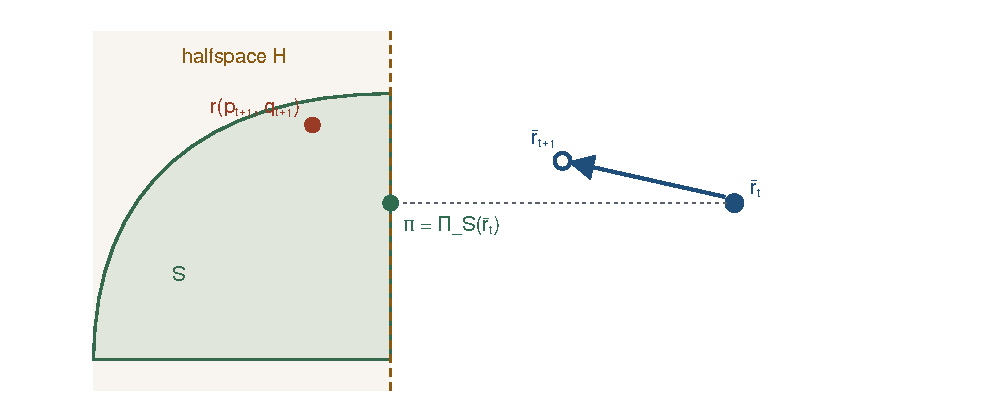
\includegraphics[width=\linewidth]{figures/ch15-fig1}
\caption*{\small One step of Blackwell's strategy. The new payoff is forced into the halfspace $H$ that supports $S$ at the projection $\pi$, so it lies on the far side of the tangent line from $\bar r_t$. The new average $\bar r_{t+1}$ moves a fraction $\frac1{t+1}$ of the way toward it, which makes its distance to $S$ shrink.}
\end{figure}

\begin{proof}[Proof of the rate]
Let $\pi=\Pi_S(\bar r_t)$ and $r=r(p_{t+1},q_{t+1})$. Since $\bar r_{t+1}=\frac{t}{t+1}\bar r_t+\frac1{t+1}r$,

\[d(\bar r_{t+1},S)^2\le\norm{\bar r_{t+1}-\pi}^2=\Big(\frac t{t+1}\Big)^2\norm{\bar r_t-\pi}^2+\frac{\norm{r-\pi}^2}{(t+1)^2}+\frac{2t}{(t+1)^2}\ip{\bar r_t-\pi}{r-\pi}.\]

The cross term is $\le0$ because $r\in H$. Multiplying by $(t+1)^2$: $(t+1)^2d_{t+1}^2\le t^2d_t^2+B^2$. Telescoping, $T^2d_T^2\le TB^2$.
\end{proof}

\section*{15.4 No-regret learning is approachability}\addcontentsline{toc}{section}{15.4 No-regret learning is approachability}\label{ch15-regret}

For the experts problem, let the learner pick $w\in\simplex_N$, the adversary pick $\ell\in[0,1]^N$, and set

\[r(w,\ell)=\big(\ip{w}{\ell}-\ell_1,\ \dots,\ \ip{w}{\ell}-\ell_N\big)\in\R^N,\qquad S=\R^N_{\le0}.\]

Coordinate $i$ of $\bar r_T$ is the average regret against expert $i$, so approaching the negative orthant is exactly vanishing regret. The response condition holds trivially: if you knew $\ell$ you would pick $e_{\argmin\ell}$. Blackwell's strategy then gives a no-regret algorithm. Working it out, the projection onto the orthant clips positive coordinates, and the forcing $p$ turns out to be $p_{t+1,i}\propto(R_{t,i})_+$: play each expert in proportion to its positive cumulative regret. This is Hart and Mas-Colell's \emph{regret matching}, the algorithm behind counterfactual regret minimisation for poker. Its regret is $O(\sqrt{NT})$ from the rate $B/\sqrt T$ with $B=O(\sqrt N)$; other potentials give Hedge's $\sqrt{T\ln N}$.

\section*{15.5 Approachability from OCO}\addcontentsline{toc}{section}{15.5 Approachability from OCO}\label{ch15-oco}

The converse direction also holds: any no-regret OCO algorithm yields an approachability strategy (Abernethy, Bartlett and Hazan 2011). The key is a dual description of distance.

\begin{bthm}{Lemma 15.5}
With support function $h_S(\theta)=\sup_{s\in S}\ip\theta s$, for every $x$: $\;d(x,S)=\max_{\norm\theta_2\le1}\big\{\ip\theta x-h_S(\theta)\big\}$.
\end{bthm}

\begin{proof}
For $\norm\theta\le1$ and any $s\in S$, $\ip{\theta}{x}-h_S(\theta)\le\ip\theta{x-\Pi_S(x)}\le d(x,S)$. For $x\notin S$ take $\theta=\frac{x-\Pi_S(x)}{d(x,S)}$; the projection optimality condition gives $\ip\theta{s-\Pi_S(x)}\le0$ for all $s\in S$, so $h_S(\theta)=\ip\theta{\Pi_S(x)}$ and equality holds. For $x\in S$ take $\theta=0$.
\end{proof}

\begin{balg}{Algorithm 15.6 \emph{(approachability via OCO)}}
\begin{algo}
maintain \ensuremath{\theta}\_t in the unit ball \ensuremath{\cap} dom(h\_S), updated by any OCO algorithm (e.g. OGD)
    \# for a cone S, dom(h\_S) is the polar cone \{\ensuremath{\theta} : \ensuremath{\langle}\ensuremath{\theta},s\ensuremath{\rangle} \ensuremath{\le} 0 for all s \ensuremath{\in} S\}
for t = 1, 2, …:
    play p\_t with \ensuremath{\langle}\ensuremath{\theta}\_t, r(p\_t, q)\ensuremath{\rangle} \ensuremath{\le} h\_S(\ensuremath{\theta}\_t) for all q     \# halfspace-forcing
    observe q\_t;  feed the OCO algorithm the convex loss
        f\_t(\ensuremath{\theta}) = h\_S(\ensuremath{\theta}) \ensuremath{-} \ensuremath{\langle}\ensuremath{\theta}, r(p\_t, q\_t)\ensuremath{\rangle}
\end{algo}
\end{balg}

Averaging, $\frac1T\sum_tf_t(\theta)=h_S(\theta)-\ip\theta{\bar r_T}$, so by Lemma 15.5, $\min_\theta\frac1T\sum_tf_t(\theta)=-d(\bar r_T,S)$. By the forcing step, $f_t(\theta_t)\ge0$. Hence $d(\bar r_T,S)\le\frac1T\big(\sum_tf_t(\theta_t)-\min_\theta\sum_tf_t(\theta)\big)=\frac{\Reg_T}{T}$. With OGD over this bounded convex domain, on which $f_t$ is convex and Lipschitz, $O(1/\sqrt T)$.

So Blackwell's theorem, no-regret learning and OCO are three presentations of one idea. Blackwell's projection strategy corresponds to running Follow the Leader on the losses $f_t$; other OCO algorithms give other approachability strategies with different constants and geometry.

\begin{bfin}{In finance}
Many portfolio mandates are sets of linear constraints on \emph{average} outcomes: tracking error to several benchmarks at once, average exposure to sectors within bands, average turnover below a cap. Each is a target set $S$ for a vector of running averages, and the market is the adversary. Blackwell's theorem gives a clean criterion: if for every market scenario there is a portfolio satisfying the mandate against that scenario, then there is an adaptive policy satisfying it on average against every sequence of scenarios, at rate $1/\sqrt T$. When the criterion fails, some scenario defeats every portfolio, and no policy can meet the mandate in the worst case. Multi-objective risk budgeting fits this framework directly.
\end{bfin}

\begin{takeaways}
\begin{itemize}
\item Vector minimax fails in one shot but holds on average: response-satisfiable convex sets are approachable.
\item Blackwell's strategy forces each new payoff into the supporting halfspace at the projection; distance falls as $B/\sqrt T$.
\item No-regret learning is approachability of the negative orthant (regret matching), and OCO algorithms give approachability strategies.
\end{itemize}
\end{takeaways}

\section*{Exercises}\addcontentsline{toc}{section}{Exercises}\label{ch15-ex}

\exercise{15.1}{\extag{easy}{warm-up}}{\hypertarget{sol-15.1}{}In the regret game of §15.4, show that for $\bar r_t\notin S$ with positive part $v=(\bar r_t)_+$, the halfspace-forcing condition is $\ip{v}{r(p,\ell)}\le0$ for all $\ell$, and that $p\propto v$ satisfies it.}

\exercise{15.2}{\extag{med}{core}}{\hypertarget{sol-15.2}{}Show that a closed convex $S$ that is not response-satisfiable is \emph{excludable}: the adversary can keep $\bar r_T$ at distance bounded below from $S$. (Blackwell's dichotomy for convex sets.)}

\exercise{15.3}{\extag{med}{core}}{\hypertarget{sol-15.3}{}Run Blackwell's strategy on Example 15.1 (the diagonal). Show that it plays $p_{t+1}=0$ when the learner's running average exceeds the adversary's, and $p_{t+1}=1$ when it is below. Compare with the strategy $p_t=q_{t-1}$.}

\subsection*{Solutions}
\begin{solutions}
\sol{15.1}{$\Pi_S(\bar r_t)=\bar r_t-v$ and $\ip{v}{\Pi_S(\bar r_t)}=0$, so $H=\{x:\ip vx\le0\}$. With $p=v/\norm v_1$: $\ip{v}{r(p,\ell)}=\sum_iv_i(\ip p\ell-\ell_i)=\norm v_1\ip p\ell-\ip v\ell=0$.}
\sol{15.2}{Some $q_0$ has $\{r(p,q_0)\}$ disjoint from $S$, with a strictly separating halfspace $\{x:\ip vx\ge c+\delta\}$ containing it while $S\subseteq\{\ip vx\le c\}$. Playing $q_0$ forever keeps every payoff, hence the average, in the first halfspace, at distance at least $\delta/\norm v$ from $S$.}
\sol{15.3}{Write $\bar r_t=(\bar x,\bar y)$. Its projection onto the diagonal is $\pi=(m,m)$ with $m=\frac{\bar x+\bar y}2$, and $v=\bar r_t-\pi=(a,-a)$ with $a=\frac{\bar x-\bar y}2$. The forcing condition $\ip{v}{(p,q)-\pi}=a(p-q)\le0$ for all $q\in[0,1]$ requires $p=0$ if $a>0$ and $p=1$ if $a<0$. Blackwell's strategy is a bang-bang controller that only looks at the averages, while $p_t=q_{t-1}$ copies the last move. Both approach the diagonal, at rates $O(1/\sqrt T)$ and $O(1/T)$ respectively.}
\end{solutions}

\chapter[Calibration and correlated equilibria]{Calibration, Internal Regret and Correlated Equilibria}\label{ch16}
\chapsource{Based on Lectures 23–24 (Dec 2 and 4, 2013) · \href{https://web.eecs.umich.edu/~jabernet/eecs598course/fall2013/web/notes/lec23_120213.pdf}{notes 23} · \href{https://web.eecs.umich.edu/~jabernet/eecs598course/fall2013/web/notes/lec24_120413.pdf}{notes 24}}

\begin{goals}
\begin{itemize}
\item What it means for probability forecasts to be calibrated, and why a forecaster facing an adversary must randomise.
\item Calibration from approachability, and approachability from calibration.
\item Internal (swap) regret, and how it makes independent learners converge to correlated equilibria.
\end{itemize}
\end{goals}

\section*{16.1 Calibrated forecasts}\addcontentsline{toc}{section}{16.1 Calibrated forecasts}\label{ch16-cal}

A weather forecaster says ``70\% chance of rain''. We cannot judge a single forecast, but we can check the long run: on the days she said about 70\%, did it rain on about 70\% of them?

\begin{bdef}{Definition 16.1 \emph{($\eps$-calibration)}}
Forecasts $p_t\in[0,1]$, outcomes $y_t\in\{0,1\}$. Fix a grid $q_1,\dots,q_N$ of spacing $\eps$ and forecasts on the grid. The forecaster is $\eps$-calibrated if the \emph{$\ell_1$ calibration score}

\[C_T=\sum_{i=1}^N\Big\lvert\frac1T\sum_{t=1}^T(q_i-y_t)\,\ind[p_t=q_i]\Big\rvert\]

satisfies $\limsup_TC_T\le c\,\eps$ for a constant $c$. Each term is the frequency of forecast $q_i$ times the gap between $q_i$ and the empirical frequency of $y=1$ on those days.
\end{bdef}

Calibration alone is a weak requirement: the forecaster who always announces the long-run base rate is calibrated on a stationary sequence and useless. It becomes interesting because it can be achieved on \emph{every} sequence, and because (as §16.2 shows) it is strong enough to derive equilibria.

\begin{bwarn}{Deterministic forecasters cannot be calibrated}
If $p_t$ is a deterministic function of the past, Nature sets $y_t=0$ when $p_t>\tfrac12$ and $y_t=1$ otherwise. Every forecast is then off by at least $\tfrac12$ on every day it is used, so $C_T\ge\tfrac12$ (Oakes 1985; Dawid 1985). The forecaster must randomise, and Nature must not see the coin flip before choosing $y_t$.
\end{bwarn}

\begin{bthm}{Theorem 16.2 \emph{(Foster and Vohra 1998)}}
There is a randomised forecaster that is $\eps$-calibrated in expectation against every adversary, for every $\eps>0$.
\end{bthm}

\begin{proof}[Proof via approachability]
The forecaster picks $\sigma\in\simplex_N$ and announces $q_I$ with $I\sim\sigma$. Nature picks $\alpha\in[0,1]$ and $y\sim\mathrm{Bernoulli}(\alpha)$. Define the vector payoff

\[r(\sigma,\alpha)=\big(\sigma_1(q_1-\alpha),\ \dots,\ \sigma_N(q_N-\alpha)\big)\in\R^N.\]

It is biaffine (so Nature's move can be taken to be the realised $y_t\in\{0,1\}$, and $r$ is computable), and each coordinate of $\bar r_T$ is the conditional expectation of the corresponding term of $C_T$; by Azuma–Hoeffding the realised terms are within $O(1/\sqrt T)$ of them, so $\E C_T\le\norm{\bar r_T}_1+O(N/\sqrt T)$. Target $S=\{x:\norm x_1\le\eps\}$, which is convex. Response condition: given $\alpha$, put all mass on the grid point nearest $\alpha$; then $r=(q_{i^*}-\alpha)e_{i^*}$ has $\ell_1$ norm at most $\eps$. By Theorem 15.3, $S$ is approachable.
\end{proof}

\section*{16.2 Calibration implies equilibrium}\addcontentsline{toc}{section}{16.2 Calibration implies equilibrium}\label{ch16-games}

Calibration generalises from $[0,1]$ to any compact convex set $Y$: partition $Y$ into $N$ cells of diameter $\eps$ with representatives $q_i$, and require that on the rounds when $q_i$ was forecast, the average outcome is within $c\eps$ of $q_i$. Now play a game by forecasting your opponent and best-responding to the forecast.

\begin{balg}{Algorithm 16.3 \emph{(calibrated best response, zero-sum game $M$)}}
\begin{algo}
for t = 1, …, T:
    forecast the opponent's mixed strategy:  q\_\{i\_t\} \ensuremath{\in} \ensuremath{\Delta}\_m  (calibrated forecaster)
    play x\_t \ensuremath{\leftarrow} argmin\_x  x\ensuremath{^{\top}} M q\_\{i\_t\}            \# best response to the forecast
    observe y\_t
\end{algo}
\end{balg}

\begin{bthm}{Theorem 16.4}
Against any sequence $y_1,y_2,\dots$, Algorithm 16.3 has average loss at most $\max_y\min_xx^\top My+O(\eps)$.
\end{bthm}

\begin{proof}
Group rounds by forecast. Let $n_i$ be the number of rounds with forecast $q_i$, and $\bar y_i$ the average of $y_t$ on them. Then

\[\frac1T\sum_tx_t^\top My_t=\sum_i\frac{n_i}{T}\,x(q_i)^\top M\bar y_i=\sum_i\frac{n_i}T\,x(q_i)^\top M(q_i+O(\eps))\le\sum_i\frac{n_i}T\min_xx^\top Mq_i+O(\eps),\]

and each $\min_xx^\top Mq_i\le\max_y\min_xx^\top My$.
\end{proof}

Combined with the trivial direction, this is another proof of the minimax theorem. The same argument with a general vector payoff (best-respond to a calibrated forecast of the opponent's move) proves Blackwell's theorem: the average payoff is a convex combination of points $r(x(q_i),q_i)\in S$, up to $O(\eps)$. So calibration and approachability are equivalent.

\section*{16.3 Correlated equilibria and internal regret}\addcontentsline{toc}{section}{16.3 Correlated equilibria and internal regret}\label{ch16-ce}

In a game with $k$ players, player $i$ picks $j_i\in[M_i]$ and suffers $C_i(j_1,\dots,j_k)$.

\begin{bdef}{Definition 16.5 \emph{(correlated equilibrium, Aumann 1974)}}
A joint distribution $\mu$ over action profiles is a correlated equilibrium if, for every player $i$ and every \emph{swap} $\varphi:[M_i]\to[M_i]$,

\[\E_{j\sim\mu}\,C_i(j)\;\le\;\E_{j\sim\mu}\,C_i\big(\varphi(j_i),j_{-i}\big).\]

Interpretation: a mediator draws $j\sim\mu$ and privately tells each player their component; no player gains by deviating from the recommendation, even as a function of it. It is an $\eps$-CE if the inequalities hold up to $\eps$.
\end{bdef}

Every Nash equilibrium (a product distribution) is a CE, but the set of CEs is a polytope defined by linear inequalities, so CEs can be computed by linear programming. In the game of Chicken, a traffic light that tells one driver ``go'' and the other ``stop'' at random is a CE that is fairer than either pure Nash equilibrium and better for both drivers than the mixed one (Exercise 16.2).

\begin{bdef}{Definition 16.6 \emph{(internal and swap regret)}}
External regret compares with always playing one fixed action. \textbf{Swap regret} compares with the best modification of one's own play by a fixed function $\varphi$:

\[\Reg^{\mathrm{swap}}_T=\max_{\varphi}\sum_{t=1}^T\sum_ip_{t,i}\big(\ell_{t,i}-\ell_{t,\varphi(i)}\big).\]

\textbf{Internal regret} restricts to $\varphi$ that changes one action $i\mapsto j$ and leaves the others alone; the two notions differ by at most a factor $N$.
\end{bdef}

External regret can be small while swap regret is linear: a learner that alternates between two actions, playing $A$ exactly when $B$ would have been better and vice versa, can match the best fixed action on average while the swap ``$A\to B,\ B\to A$'' would have been perfect.

\begin{bthm}{Theorem 16.7 \emph{(Foster and Vohra 1997; Hart and Mas-Colell 2000)}}
If every player uses an algorithm with swap regret $o(T)$, the empirical distribution of joint play $\bar\mu_T=\frac1T\sum_t\mu_t$ converges to the set of correlated equilibria. With swap regret $R_T$, $\bar\mu_T$ is an $R_T/T$-correlated equilibrium.
\end{bthm}

\begin{proof}
Player $i$'s losses on round $t$ are induced by the others' play. Its swap-regret bound reads $\frac1T\sum_t\big(C_i(\mu_t)-C^\varphi_i(\mu_t)\big)\le R_T/T$ for every $\varphi$. Both $C_i(\mu)$ and $C_i^\varphi(\mu)$ are linear in $\mu$, so this is $C_i(\bar\mu_T)\le C_i^\varphi(\bar\mu_T)+R_T/T$.
\end{proof}

\subsection*{Getting low swap regret}

\emph{Via approachability.} Use the $N^2$-dimensional payoff $r(w,\ell)_{(i,j)}=w_i(\ell_i-\ell_j)$ with target the negative orthant. Coordinate $(i,j)$ of the average is the regret for the swap $i\mapsto j$. The response condition holds with $w=e_{\argmin\ell}$, so Blackwell's theorem gives $o(T)$ internal regret.

\emph{Via external regret (Blum and Mansour 2007).} Run $N$ copies $A_1,\dots,A_N$ of Hedge. Each outputs a distribution $q^{(i)}_t$; stack them as the rows of a stochastic matrix $Q_t$ and play its stationary distribution $p_t=p_tQ_t$. Feed copy $A_i$ the loss vector $p_{t,i}\ell_t$. Then

\[\Reg^{\mathrm{swap}}_T\;\le\;\sum_{i=1}^N\Reg_T(A_i)\;=\;O\big(\sqrt{NT\ln N}\big).\]

The stationarity condition $p_t=p_tQ_t$ is what makes ``play $p_t$'' and ``let copy $i$ choose where action $i$'s mass goes'' the same thing.

\section*{16.4 The map of the course}\addcontentsline{toc}{section}{16.4 The map of the course}\label{ch16-map}

\begin{figure}[htbp]
\centering
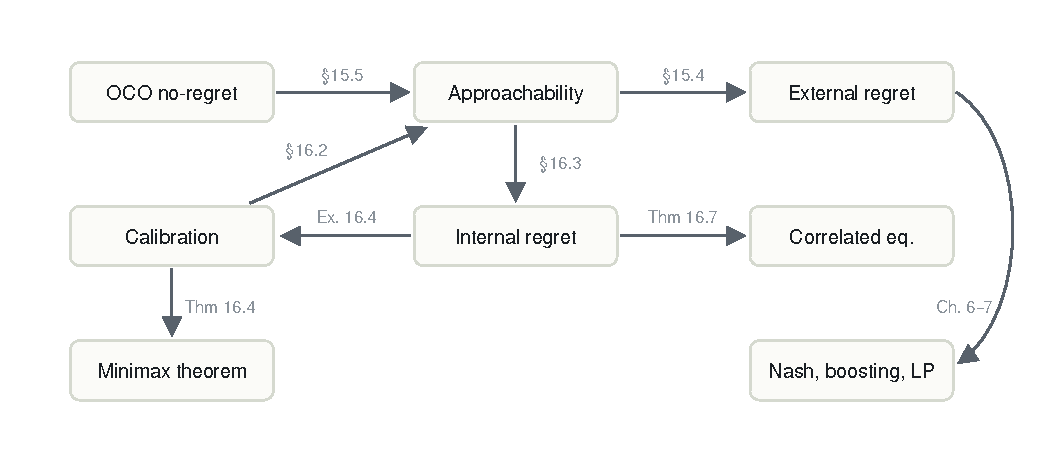
\includegraphics[width=\linewidth]{figures/ch16-fig1}
\caption*{\small How the main results of the course imply one another. An arrow from A to B means an algorithm for A yields an algorithm or constructive proof for B.}
\end{figure}

\begin{bfin}{In finance}
Calibration is the everyday test of probability forecasts in finance: are 2\%-PD obligors defaulting at 2\%? Do option-implied probabilities of a 10\% move match realised frequencies? Rating agencies and model validators publish exactly the reliability tables of Definition 16.1. Theorem 16.2 has a sobering reading: calibration on its own can be achieved by a forecaster who knows nothing about credit, just by adjusting forecasts to past frequencies with randomisation. So calibration is necessary but far from sufficient, and good forecasts must also be \emph{sharp} (discriminating), as measured by a proper scoring rule such as the Brier or log score (Chapter 3). Prediction markets aggregate beliefs through the same scoring rules: a market maker using a logarithmic market scoring rule (Hanson) is running a cost function equal to the softmin potential of Chapter 3, which connects market making to online learning (Abernethy, Chen and Wortman Vaughan 2013).
\end{bfin}

\begin{takeaways}
\begin{itemize}
\item Calibration is achievable against any adversary, but only by randomised forecasters.
\item Calibration \ensuremath{\Leftrightarrow} approachability, and best-responding to calibrated forecasts proves the minimax theorem.
\item Swap (internal) regret is the right notion for multi-player games: when all players have low swap regret, play converges to the set of correlated equilibria.
\item Blum–Mansour turns any $N$ external-regret algorithms into one with low swap regret.
\end{itemize}
\end{takeaways}

\section*{Exercises}\addcontentsline{toc}{section}{Exercises}\label{ch16-ex}

\exercise{16.1}{\extag{easy}{warm-up}}{\hypertarget{sol-16.1}{}A forecaster announces $0.3$ on $100$ days (rain on $36$) and $0.8$ on $50$ days (rain on $36$). Compute $C_T$.}

\exercise{16.2}{\extag{med}{core}}{\hypertarget{sol-16.2}{}In Chicken, each driver chooses Go or Stop. Losses: both Go $10$; Go vs Stop: $0$ for Go and $2$ for Stop; both Stop $3$. Find the mixed Nash equilibrium, and show the ``traffic light'' distribution $\mu=\frac12(\text{Go},\text{Stop})+\frac12(\text{Stop},\text{Go})$ is a correlated equilibrium with lower expected loss.}

\exercise{16.3}{\extag{med}{core}}{\hypertarget{sol-16.3}{}Prove the Blum–Mansour bound. Hint: copy $i$'s regret against action $j$ is $\sum_tp_{t,i}(\ip{q^{(i)}_t}{\ell_t}-\ell_{t,j})$, and stationarity gives $\sum_ip_{t,i}\ip{q^{(i)}_t}{\ell_t}=\ip{p_tQ_t}{\ell_t}=\ip{p_t}{\ell_t}$.}

\exercise{16.4}{\extag{hard}{challenge}}{\hypertarget{sol-16.4}{}(Lecture 24.) Show that no-internal-regret implies calibration: treat grid points as experts with loss $(q_i-y_t)^2$, and show that a miscalibrated forecast bin can be profitably swapped to the grid point nearest its empirical frequency.}

\subsection*{Solutions}
\begin{solutions}
\sol{16.1}{$T=150$. Terms: $\frac{100}{150}\abs{0.3-0.36}=0.04$ and $\frac{50}{150}\abs{0.8-0.72}=0.0267$. $C_T\approx0.067$.}
\sol{16.2}{Mixed Nash: if the other goes with probability $g$, Go costs $10g$ and Stop costs $2g+3(1-g)=3-g$. Indifference gives $g=3/11$ and expected loss $30/11\approx2.73$ each. Under $\mu$, a player told Stop knows the other goes: Stop costs $2$, Go costs $10$, so obey. A player told Go knows the other stops: Go costs $0$, Stop costs $3$, so obey. Expected loss is $\frac12(0)+\frac12(2)=1$ each.}
\sol{16.3}{For any $\varphi$, sum copy $i$'s regret against $\varphi(i)$ over $i$: $\sum_i\sum_tp_{t,i}(\ip{q_t^{(i)}}{\ell_t}-\ell_{t,\varphi(i)})=\sum_t\ip{p_t}{\ell_t}-\sum_t\sum_ip_{t,i}\ell_{t,\varphi(i)}$, which is the swap regret for $\varphi$. Each copy has regret $O(\sqrt{T\ln N})$ on losses in $[0,1]$ (scaled by $p_{t,i}\le1$), and a sharper analysis using $\sum_i\sqrt{\sum_tp_{t,i}}\le\sqrt{NT}$ gives $O(\sqrt{NT\ln N})$.}
\end{solutions}

\def\thepartblurb{Two chapters that take the theory to the trading desk: learning rates that tune themselves, and what regret bounds do and do not promise a portfolio.}\part{Online Learning for Investors}\label{part7}

\chapter[Adaptive learning rates and AdaHedge]{Adaptive Learning Rates and AdaHedge}\label{ch17}
\chapsource{Beyond the course · de Rooij, van Erven, Grünwald and Koolen, ``Follow the leader if you can, Hedge if you must'', \emph{JMLR} 2014 · Cesa-Bianchi, Mansour and Stoltz, ``Improved second-order bounds for prediction with expert advice'', \emph{Machine Learning} 2007}

\begin{goals}
\begin{itemize}
\item Why every Hedge bound so far needed a quantity you do not have: $T$, $L^*$, or the variance of the losses.
\item The mix loss and the mixability gap: a decomposition of Hedge's loss that works for any sequence of learning rates.
\item AdaHedge, which sets $\eta_t=\ln N/\Delta_{t-1}$ from the gaps it has already paid, and its parameter-free regret bound.
\item What adaptivity buys when the ``experts'' are trading signals.
\end{itemize}
\end{goals}

\section*{17.1 The tuning problem}\addcontentsline{toc}{section}{17.1 The tuning problem}\label{ch17-tuning}

Every bound for exponential weights has come with a learning rate to tune. Theorem 2.4 wants $\eps^*=\sqrt{2\ln N/M_T(i)}$; Corollary 3.5 wants $L^*$; Theorem 3.8 wants $T$. Two fixes were mentioned in Chapter 2: the \emph{doubling trick} (Exercise 2.4), which guesses $T$, restarts each time the guess is exceeded and pays a factor $\frac{\sqrt2}{\sqrt2-1}\approx3.4$; and a \emph{time-varying rate} $\eta_t\propto1/\sqrt t$, which we have not yet analysed because the potential argument of Chapter 3 needs a fixed $\eta$. Neither fix addresses the real issue: on easy data (one signal clearly best, or losses that vary little) the right $\eta$ is large and the regret should be far below $\sqrt{T\ln N}$, while on hard data it should be small. A tuning rule that looks only at $T$ cannot tell the two apart.

\begin{bfin}{In finance: a learning rate is a memory length}
Weights $\propto e^{-\eta L_{i,t}}$ forget nothing, but $\eta$ decides how much a unit of past loss matters. With $\eta$ large the allocation snaps to the current leader after a few days: short memory, fast reaction, and whipsaw when signals trade places. With $\eta$ small it takes hundreds of days of outperformance to move the weights: long memory, slow reaction. Practitioners tune this by backtest, which is the data-snooping problem of Chapter 5 in another guise. An algorithm that sets $\eta$ from what the data have already cost it removes one knob from the backtest.
\end{bfin}

\section*{17.2 Mix loss and the mixability gap}\addcontentsline{toc}{section}{17.2 Mix loss and the mixability gap}\label{ch17-mix}

Return to the Hedge setting (Protocol 3.6): losses $\ell_{t,i}\in[0,1]$, cumulative losses $L_{i,t}=\sum_{s\le t}\ell_{s,i}$, and the learner plays $p_t$ with $p_{t,i}\propto e^{-\eta_tL_{i,t-1}}$ for a rate $\eta_t>0$ that may now change with $t$. The learner pays $h_t=\ip{p_t}{\ell_t}$. The key device is to compare $h_t$ with a quantity that telescopes.

\begin{bdef}{Definition 17.1 \emph{(mix loss, mixability gap)}}
With weights $p_t$ and learning rate $\eta_t$, the \textbf{mix loss} and the \textbf{mixability gap} of round $t$ are

\[m_t=-\frac1{\eta_t}\ln\sum_{i=1}^Np_{t,i}e^{-\eta_t\ell_{t,i}},\qquad \delta_t=h_t-m_t,\]

with cumulative versions $M_T=\sum_{t\le T}m_t$, $H_T=\sum_{t\le T}h_t$ and $\Delta_T=\sum_{t\le T}\delta_t$. So $H_T=M_T+\Delta_T$. (For $\eta_t=\infty$ the weights sit uniformly on the current leaders and $m_t$ is the smallest loss among them.)
\end{bdef}

The mix loss is what the learner would pay if it could ``mix'' the experts' losses through the exponential rather than average them: it is the log-loss of a Bayesian mixture (Exercise 3.5), and in the proof of Theorem 3.4 it is exactly the increase of the softmin potential, $m_t=\Phi_{\eta_t}(L_t)-\Phi_{\eta_t}(L_{t-1})$. Two facts about it do all the work.

\begin{bthm}{Lemma 17.2 \emph{(mix loss telescopes)}}
If $\eta_1\ge\eta_2\ge\dots\ge\eta_T$, then for every expert $i$,

\[M_T\;\le\;L_{i,T}+\frac{\ln N}{\eta_T}.\]

\end{bthm}

\begin{proof}
Write $\Phi_t(\eta)=-\frac1\eta\ln\frac1N\sum_ie^{-\eta L_{i,t}}$ for the softmin of Section 3.3 with the uniform prior, so $\Phi_0(\eta)=0$ and $m_t=\Phi_t(\eta_t)-\Phi_{t-1}(\eta_t)$. Then

\[M_T=\Phi_T(\eta_T)+\sum_{t=1}^{T-1}\big[\Phi_t(\eta_t)-\Phi_t(\eta_{t+1})\big].\]

$\Phi_t(\eta)$ is nonincreasing in $\eta$ (Exercise 17.2: it interpolates between the mean of the $L_{i,t}$ at $\eta\to0$ and their minimum at $\eta\to\infty$), and $\eta_{t+1}\le\eta_t$, so every bracket is $\le0$. Finally $\Phi_T(\eta_T)\le-\frac1{\eta_T}\ln\frac1Ne^{-\eta_TL_{i,T}}=L_{i,T}+\frac{\ln N}{\eta_T}$.
\end{proof}

With a fixed $\eta$ this is the potential argument of Chapter 3 in one line. The point is that it survives a decreasing learning rate at no cost: only the last $\eta_T$ appears.

\begin{bthm}{Lemma 17.3 \emph{(the gap is small)}}
For losses in $[0,1]$ and any $\eta_t>0$, with $s_t=\sum_ip_{t,i}\ell_{t,i}^2$:

\begin{enumerate}
\item $0\le\delta_t\le1$;
\item $\delta_t\le\eta_t/8$;
\item $\delta_t\le\tfrac12\eta_t\,s_t\le\tfrac12\eta_t\,h_t$.
\end{enumerate}
\end{bthm}

\begin{proof}
Let $X$ take the value $\ell_{t,i}$ with probability $p_{t,i}$, so $h_t=\E X$ and $m_t=-\frac1{\eta}\ln\E e^{-\eta X}$ (writing $\eta$ for $\eta_t$). (1) Jensen gives $\E e^{-\eta X}\ge e^{-\eta\E X}$, i.e. $m_t\le h_t$; and $m_t\ge\min_i\ell_{t,i}\ge0$, $h_t\le1$. (2) Hoeffding's lemma (Lemma 3.7) with $s=-\eta$: $\ln\E e^{-\eta(X-\E X)}\le\eta^2/8$, i.e. $m_t\ge h_t-\eta/8$. (3) For $x\ge0$, $e^{-x}\le1-x+x^2/2$, so $\E e^{-\eta X}\le1-\eta h_t+\tfrac12\eta^2s_t=:u$. Then $m_t=-\frac1\eta\ln u\ge-\frac1\eta(u-1)=h_t-\tfrac12\eta s_t$ by (I2). Since $\ell^2\le\ell$ on $[0,1]$, $s_t\le h_t$.
\end{proof}

Putting the two lemmas together: for any nonincreasing rates, $\Reg_T=H_T-L^*_T\le\frac{\ln N}{\eta_T}+\Delta_T$. The first term wants $\eta_T$ large, the gap wants the $\eta_t$ small, and the bounds on $\delta_t$ say how the two trade off. The simplest use is the time-varying rate.

\begin{bthm}{Corollary 17.4 \emph{(time-varying Hedge)}}
Hedge with $\eta_t=\sqrt{8\ln N/t}$ has, simultaneously for every $T$,

\[\Reg_T\;\le\;\Big(\frac1{2\sqrt2}+\frac1{\sqrt2}\Big)\sqrt{T\ln N}\;<\;1.07\sqrt{T\ln N}.\]

\end{bthm}

\begin{proof}
$\frac{\ln N}{\eta_T}=\sqrt{T\ln N/8}$, and by Lemma 17.3(2), $\Delta_T\le\frac18\sum_{t\le T}\sqrt{8\ln N/t}\le\frac{\sqrt{8\ln N}}8\cdot2\sqrt T=\sqrt{T\ln N/2}$.
\end{proof}

That is $1.5$ times the tuned constant of Theorem 3.8, with no knowledge of $T$ and no restarts. But it still ignores the data: $\eta_t$ falls like $1/\sqrt t$ whether the gaps have been large or zero.

\section*{17.3 AdaHedge}\addcontentsline{toc}{section}{17.3 AdaHedge}\label{ch17-adahedge}

The regret bound $\frac{\ln N}{\eta_T}+\Delta_T$ suggests balancing the two terms \emph{as they are realised}: choose $\eta_t$ so that $\ln N/\eta_t$ equals the gap already accumulated.

\begin{balg}{Algorithm 17.5 \emph{(AdaHedge, de Rooij, van Erven, Grünwald and Koolen 2014)}}
\begin{algo}
\ensuremath{\Delta}\_0 \ensuremath{\leftarrow} 0
for t = 1, 2, …:
    \ensuremath{\eta}\_t \ensuremath{\leftarrow} ln N / \ensuremath{\Delta}\_\{t\ensuremath{-}1\}            \# \ensuremath{\eta}\_1 = \ensuremath{\infty}: Follow the Leader, uniform over leaders
    p\_\{t,i\} \ensuremath{\propto} exp(\ensuremath{-}\ensuremath{\eta}\_t L\_\{i,t\ensuremath{-}1\})
    observe \ensuremath{\ell}\_t;  h\_t \ensuremath{\leftarrow} \ensuremath{\Sigma}\_i p\_\{t,i\} \ensuremath{\ell}\_\{t,i\}
    m\_t \ensuremath{\leftarrow} \ensuremath{-}(1/\ensuremath{\eta}\_t) ln \ensuremath{\Sigma}\_i p\_\{t,i\} exp(\ensuremath{-}\ensuremath{\eta}\_t \ensuremath{\ell}\_\{t,i\})
    \ensuremath{\Delta}\_t \ensuremath{\leftarrow} \ensuremath{\Delta}\_\{t\ensuremath{-}1\} + (h\_t \ensuremath{-} m\_t)
\end{algo}

$\Delta_t$ is nondecreasing, so $\eta_t$ is nonincreasing and Lemma 17.2 applies. The cost per round is $O(N)$, the same as Hedge.
\end{balg}

\begin{bthm}{Theorem 17.6 \emph{(AdaHedge regret)}}
For losses in $[0,1]$, AdaHedge satisfies, with $S_T=\sum_{t\le T}\sum_ip_{t,i}\ell_{t,i}^2\le H_T\le T$,

\[\Reg_T\;\le\;2\Delta_T\;\le\;2\sqrt{S_T\ln N}+2\;\le\;2\sqrt{T\ln N}+2.\]

\end{bthm}

\begin{proof}
By Lemma 17.2 and the choice of $\eta_T$, $\Reg_T\le\frac{\ln N}{\eta_T}+\Delta_T=\Delta_{T-1}+\Delta_T\le2\Delta_T$. To bound $\Delta_T$, look at how $\Delta_t^2$ grows:

\[\Delta_t^2-\Delta_{t-1}^2=2\Delta_{t-1}\delta_t+\delta_t^2\;\le\;2\Delta_{t-1}\cdot\frac{\eta_ts_t}{2}+\delta_t\;=\;s_t\ln N+\delta_t,\]

using Lemma 17.3(3) for the first term (when $\Delta_{t-1}=0$ the first term is $0$ anyway) and $\delta_t^2\le\delta_t$ from Lemma 17.3(1). Summing over $t$, $\Delta_T^2\le S_T\ln N+\Delta_T$. A number $x\ge0$ with $x^2-x\le c$ satisfies $x\le\frac{1+\sqrt{1+4c}}2\le1+\sqrt c$, which gives $\Delta_T\le\sqrt{S_T\ln N}+1$.
\end{proof}

\begin{bthm}{Corollary 17.7 \emph{(parameter-free small-loss bound)}}
For losses in $[0,1]$, AdaHedge has $\;\Reg_T\le2\sqrt{L^*_T\ln N}+5\ln N+4$, where $L^*_T=\min_iL_{i,T}$.
\end{bthm}

\begin{proof}
$S_T\le H_T=L^*_T+\Reg_T$, so Theorem 17.6 gives $\Reg_T\le2\sqrt{(L^*_T+\Reg_T)\ln N}+2$: the regret appears on both sides, and solving the quadratic (Exercise 17.5) gives the claim.
\end{proof}

Compare Corollary 3.5, $\sqrt{2L^*\ln N}+\ln N$, which needed $L^*$ in advance: AdaHedge gets the same $\sqrt{L^*\ln N}$ shape with no input at all. When one expert is perfect ($L^*=0$) the regret is $O(\ln N)$, like Halving; when every expert is mediocre it is $O(\sqrt{T\ln N})$, like tuned Hedge; and the algorithm did not need to be told which case it was in. De Rooij et al. prove a sharper version of Lemma 17.3 in terms of the \emph{variance} $v_t$ of the loss under $p_t$ rather than the second moment, giving $\Reg_T\le2\sqrt{V_T\ln N}+\frac43\ln N+2$ with $V_T=\sum_tv_t\le T/4$: within a factor $\sqrt2$ of the tuned constant on hard data, and much better whenever the experts agree.

\begin{bwarn}{What AdaHedge is not}
It is not a doubling trick: it never restarts and never discards data. It is not a fixed schedule: $\eta_t$ is a function of the losses, and on easy sequences it stays large (the algorithm behaves like Follow the Leader). And it is not free of assumptions: the bounds use $\ell\in[0,1]$, so losses must be scaled, and a single huge loss will shrink $\eta$ for a long time. De Rooij et al. also give FlipFlop, which alternates between AdaHedge and Follow the Leader and inherits the better of the two guarantees.
\end{bwarn}

\begin{figure}[htbp]
\centering
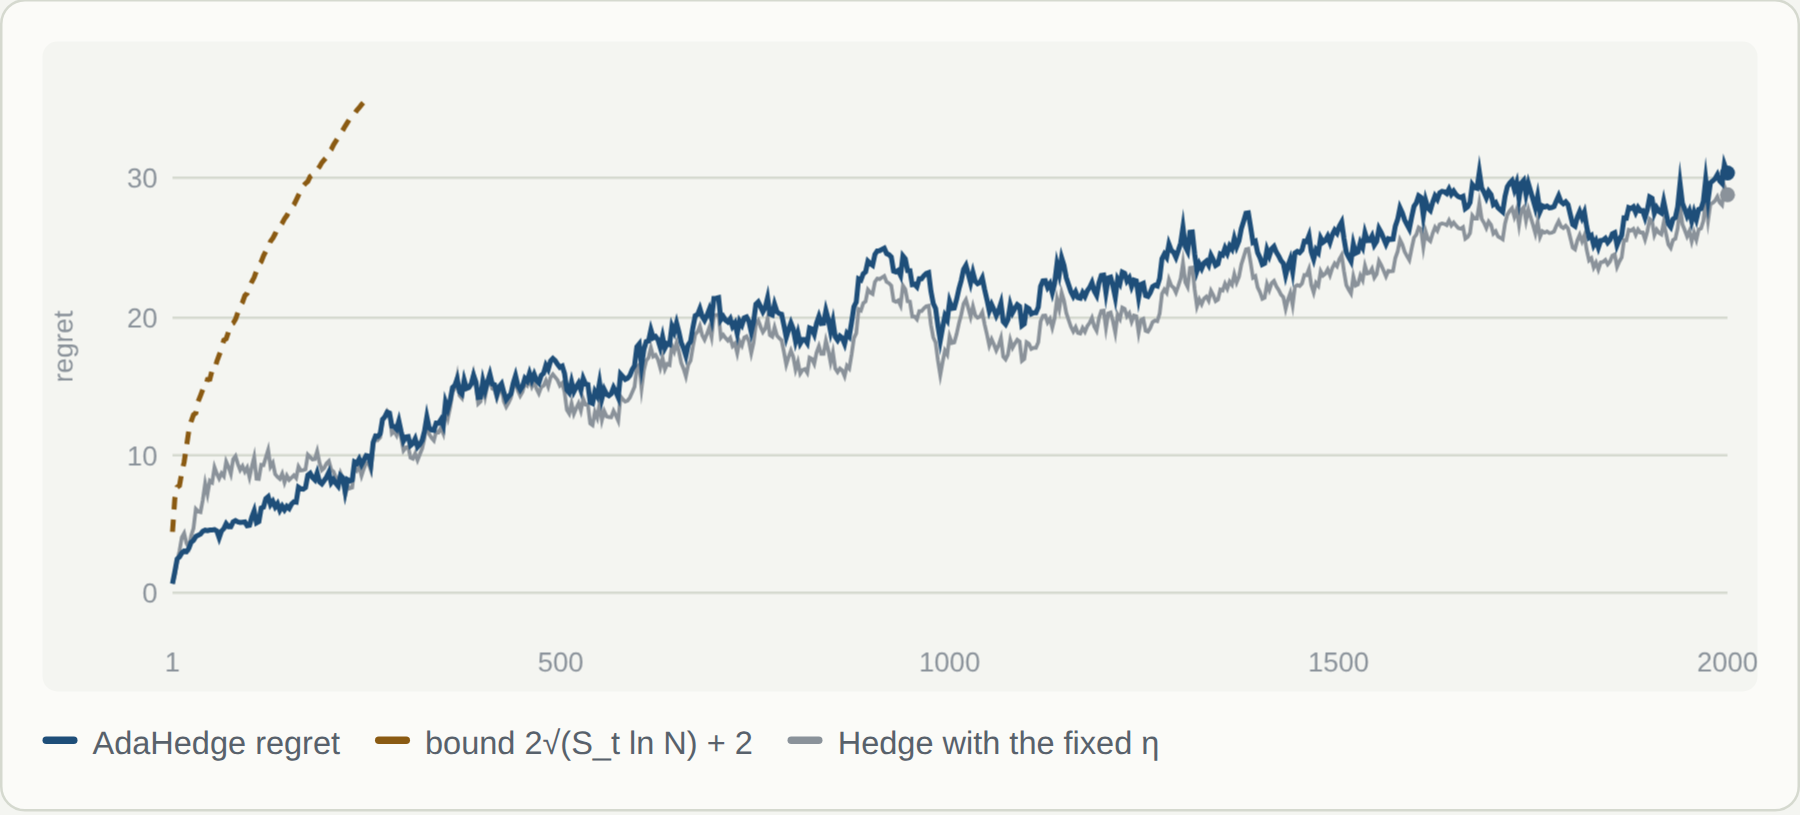
\includegraphics[width=\linewidth]{figures/demo-ada}
\caption*{\small The same simulated market as the Chapter 3 demo ($N$ signals, $T=2000$ days, drifting Bernoulli losses, the current leader periodically punished). Move the slider to see how sensitive fixed-rate Hedge is to $\eta$; AdaHedge has no slider. Its learning rate at the end of the run is shown in the readout: on this market it usually lands near the rate you would have tuned by hand, without being told $T$. \emph{(A static snapshot at the default settings; the HTML edition has live sliders.)}}
\end{figure}

\section*{17.4 Beyond AdaHedge}\addcontentsline{toc}{section}{17.4 Beyond AdaHedge}\label{ch17-beyond}

AdaHedge is one member of a family of \emph{parameter-free} or \emph{adaptive} methods that has grown rapidly since the course was given. Three are worth knowing.

\begin{itemize}
\item \textbf{Second-order bounds.} Cesa-Bianchi, Mansour and Stoltz (2007) obtain regret $O\big(\sqrt{\sum_t\mathrm{Var}_{p_t}(\ell_t)\,\ln N}+\ln N\big)$ with a tuned rate; AdaHedge achieves it without tuning. When all signals have similar daily losses, as diversified strategies often do, the variance term is far below $T/4$.
\item \textbf{Quantile and Squint bounds.} Koolen and van Erven (2015) replace $\ln N$ by $\ln(1/\pi(\text{good experts}))$: if a constant fraction of a large library is nearly as good as the best, the regret does not grow with the library size at all. Chapter 5's data-snooping haircut $\sqrt{(T/2)\ln N}$ is then an overestimate.
\item \textbf{Coin betting.} Orabona and Pál (2016) turn parameter-free OCO into a betting problem: a learner that bets on the sign of the gradients with a Kelly-like fraction (Chapter 11) achieves $O\big(\norm u\sqrt{T\ln(1+\norm uT)}\big)$ regret against every comparator $u$ at once, with no step size. It is the online-learning counterpart of the ``bet a fraction of wealth'' rule and closes a loop between Parts III and IV.
\end{itemize}

\begin{bfin}{In finance: a fund of signals}
Suppose a desk runs $N$ forecasting models for tomorrow's return, each producing a number in $[-1,1]$, and scores them by a bounded loss such as $\ell(f,r)=\tfrac12\abs{f-\mathrm{sign}(r)}$ or a clipped squared error. AdaHedge on these losses is a model-combination rule with no lookback window and no learning rate to backtest, and Corollary 17.7 says its cumulative score is within $2\sqrt{L^*\ln N}+O(\ln N)$ of the best model in hindsight. If the models are strategies that reinvest wealth, the natural loss is $-\ln(\text{wealth relative})$ and the natural combination is buy-and-hold across strategies (Exercise 17.4), which is AdaHedge's fixed point at $\eta=1$: for log loss the mixability gap is zero (Exercise 3.5), so no learning rate needs to be learned. Regime changes are still Fixed Share's job (Chapter 4); the two ideas combine, with AdaHedge choosing $\eta$ and the switching prior choosing $\alpha$.
\end{bfin}

\begin{takeaways}
\begin{itemize}
\item Hedge's loss splits as $H_T=M_T+\Delta_T$: a mix loss that telescopes to $L^*+\ln N/\eta_T$ for any nonincreasing rates, plus a gap $\delta_t\le\min\{1,\eta_t/8,\eta_th_t/2\}$.
\item Setting $\eta_t=\ln N/\Delta_{t-1}$ balances the two terms online. AdaHedge's regret is at most $2\Delta_T\le2\sqrt{S_T\ln N}+2$, hence $2\sqrt{L^*\ln N}+O(\ln N)$, with nothing to tune.
\item Adaptivity means paying for the difficulty the data actually had, not the difficulty they might have had.
\end{itemize}
\end{takeaways}

\section*{Exercises}\addcontentsline{toc}{section}{Exercises}\label{ch17-ex}

\exercise{17.1}{\extag{easy}{warm-up}}{\hypertarget{sol-17.1}{}For finite $\eta_t$, show that $\delta_t=0$ if and only if every expert with positive weight has the same loss in round $t$. What does this say about the sequences on which AdaHedge keeps $\eta_t=\infty$ forever?}

\exercise{17.2}{\extag{med}{core}}{\hypertarget{sol-17.2}{}Prove that $\Phi(\eta)=-\frac1\eta\ln\frac1N\sum_ie^{-\eta L_i}$ is nonincreasing in $\eta>0$, with limits $\frac1N\sum_iL_i$ as $\eta\to0$ and $\min_iL_i$ as $\eta\to\infty$.}

\exercise{17.3}{\extag{med}{core}}{\hypertarget{sol-17.3}{}(Realizable case.) One expert has loss $0$ in every round. Use Corollary 17.7 to bound AdaHedge's regret and compare with Halving (Theorem 1.4) and with Hedge at the rate $\eta=\sqrt{8\ln N/T}$.}

\exercise{17.4}{\extag{fin}{finance}}{\hypertarget{sol-17.4}{}(A fund of strategies.) $K$ strategies have wealth paths $W_{k,t}$, all starting at $1$. Split capital equally and let each run with no transfers (``buy and hold across strategies''). (a) Show that the fund's wealth satisfies $\ln W_T\ge\max_k\ln W_{k,T}-\ln K$. (b) Show this is EWA with $\eta=1$ on the losses $\ell_{t,k}=-\ln(W_{k,t}/W_{k,t-1})$, and that its mixability gap is zero. (c) In the Chapter 11 demo the universal portfolio is exactly this fund over $K=201$ grid CRPs. Compare $\ln 201$ with the guarantee $1+\ln(T+1)$ of Theorem 11.4 for $T=2520$, and explain what the fund's bound does not cover.}

\exercise{17.5}{\extag{hard}{challenge}}{\hypertarget{sol-17.5}{}Derive Corollary 17.7: show that $R\le2\sqrt{(L+R)a}+2$ with $a=\ln N$ implies $R\le2\sqrt{La}+5a+4$.}

\subsection*{Solutions}
\begin{solutions}
\sol{17.1}{$\delta_t=0$ is equality in Jensen's inequality $\E e^{-\eta X}\ge e^{-\eta\E X}$, which holds for the strictly convex exponential iff $X$ is constant on the support of $p_t$. With $\eta_1=\infty$ the weights are uniform over the current leaders; $\Delta$ stays $0$ exactly as long as all leaders take the same loss each round, so Follow the Leader is played until the first round in which the leaders disagree.}
\sol{17.2}{For $0<\eta<\eta'$, the map $u\mapsto u^{\eta'/\eta}$ is convex, so by Jensen $\big(\frac1N\sum_ie^{-\eta L_i}\big)^{\eta'/\eta}\le\frac1N\sum_ie^{-\eta'L_i}$. Taking $-\frac1{\eta'}\ln$ of both sides reverses the inequality: $\Phi(\eta)\ge\Phi(\eta')$. The limits: $-\frac1\eta\ln\E e^{-\eta L}=\E L-\frac\eta2\mathrm{Var}(L)+O(\eta^2)$ as $\eta\to0$, and $\frac1N e^{-\eta\min L}\le\frac1N\sum e^{-\eta L_i}\le e^{-\eta\min L}$ gives $\min L\le\Phi(\eta)\le\min L+\frac{\ln N}\eta$.}
\sol{17.3}{$L^*=0$, so AdaHedge's regret (here, its total loss) is at most $5\ln N+4=O(\ln N)$, the same order as Halving's $\log_2N$ mistakes, though Halving is deterministic and exploits the realizability. Hedge tuned for the worst case pays up to $\sqrt{(T/2)\ln N}$, which for $T=2000$, $N=10$ is about $48$ versus AdaHedge's $15.5$. The first-order bound is what recovers the easy case; AdaHedge gets it without being told the case is easy.}
\sol{17.4}{(a) $W_T=\frac1K\sum_kW_{k,T}\ge\frac1K\max_kW_{k,T}$. (b) The fund's weight on strategy $k$ at time $t$ is $W_{k,t-1}/\sum_jW_{j,t-1}=e^{-L_{k,t-1}}/\sum_je^{-L_{j,t-1}}$, which is EWA with $\eta=1$. Its per-round loss is $-\ln(W_t/W_{t-1})=-\ln\sum_kp_{t,k}e^{-\ell_{t,k}}=m_t$: the mix loss itself, so $\delta_t=0$ and Lemma 17.2 gives (a) again. (c) $\ln201\approx5.3$ against $1+\ln2521\approx8.8$. The fund's bound is against the best \emph{grid} CRP; the continuous best CRP can be slightly better than its nearest grid point, and that discretization error, not the $\ln K$, is what Theorem 11.4's integral handles.}
\sol{17.5}{If $R<2$ there is nothing to prove; otherwise set $x=R-2\ge0$. Squaring, $x^2\le4a(L+x+2)$, i.e. $x^2-4ax-(4aL+8a)\le0$, so $x\le2a+\sqrt{4a^2+4aL+8a}\le2a+2a+2\sqrt{aL}+\sqrt{8a}$, using $\sqrt{u+v+w}\le\sqrt u+\sqrt v+\sqrt w$. Finally $\sqrt{8a}=2\sqrt{2a}\le a+2$ by AM–GM, so $R\le2\sqrt{aL}+5a+4$.}
\end{solutions}

\chapter[Portfolio selection in practice]{Portfolio Selection in Practice}\label{ch18}
\chapsource{Beyond the course · Cover and Ordentlich, ``Universal portfolios with side information'', \emph{IEEE Trans. Inf. Theory} 1996 · Blum and Kalai, ``Universal portfolios with and without transaction costs'', \emph{Machine Learning} 1999 · MacLean, Thorp and Ziemba (eds.), \emph{The Kelly Capital Growth Investment Criterion}, 2011}

\begin{goals}
\begin{itemize}
\item How to read a regret bound for a portfolio: what $(n-1)\ln T$ promises over ten years of daily data, and why the realised gap is far smaller.
\item Transaction costs: a back-of-the-envelope rule for when rebalancing pays, and what survives of the universal guarantee.
\item Side information and regime switches: the tools of Chapters 4 and 11 combined.
\item Risk: log-optimal is not risk-free, fractional Kelly, and why Sharpe ratios have no regret theory.
\item A checklist for using online learning on a trading desk.
\end{itemize}
\end{goals}

\section*{18.1 Reading the guarantee}\addcontentsline{toc}{section}{18.1 Reading the guarantee}\label{ch18-reading}

Theorem 11.4 promises $\ln W_T(x^*)-\ln W_T(\mathrm{UP})\le(n-1)\ln(T+1)+1$ on every sequence. Put in numbers: ten years of daily data is $T=2520$, and with $n=10$ assets the bound is $9\ln2521+1\approx71.5$ nats. That is a factor $e^{71}$ in wealth, or $7$ nats per year: as a promise about a decade it is empty. Even the minimax-optimal Dirichlet$(\tfrac12)$ version, $\frac{n-1}2\ln(T+1)+\ln2\approx36$, is empty. Yet the Chapter 11 demo, with $n=2$ and a guarantee of $1+\ln2521\approx8.8$, shows a realised gap of a few hundredths. Both facts are true, and the difference between them is the whole art of using these bounds.

The worst-case bound is attained only by sequences that make the best CRP extremely sharp: price relatives that swing by factors of two, so that a small move away from $x^*$ costs a large fraction of wealth every day. Real daily price relatives lie within a percent or two of $1$, and then $\ln W_T(x)$ is a very flat function of $x$. Exercise 11.5 makes this quantitative by Laplace's method: near an interior maximiser, $\ln W_T(x)\approx\ln W_T(x^*)-\tfrac T2(x-x^*)^\top\Sigma(x-x^*)$ with $\Sigma$ the sample covariance of the price relatives, and averaging $W_T(x)$ over the simplex gives

\[\ln W_T(x^*)-\ln W_T(\mathrm{UP})\;\approx\;\frac{n-1}2\ln\frac{T\sigma^2}{2\pi}+O(1),\]

where $\sigma^2$ is the scale of the daily variance. The effective horizon is not $T$ but $T\sigma^2$, the number of days times the daily variance: for equities $\sigma\approx1.5\%$ per day, so $T\sigma^2\approx0.57$ over the decade and the logarithm is not even positive. The universal portfolio is within $O(1)$ nats of the best CRP on realistic data, because the best CRP is barely identifiable from the data in the first place.

\begin{bwarn}{Two readings of one bound}
As a \emph{guarantee}, $(n-1)\ln T$ says: whatever happens, including a crash engineered against you, you lose at most this much log-wealth to the best rebalancing rule. As a \emph{prediction} of the realised gap on ordinary data it is useless, and should not be used to size positions or set expectations. The same is true of every bound in this book: they are insurance, and the premium is that the algorithm hedges across comparators it will not need. Whether the insurance is worth its price is an empirical question about your market, not a theorem.
\end{bwarn}

\section*{18.2 Transaction costs}\addcontentsline{toc}{section}{18.2 Transaction costs}\label{ch18-costs}

A CRP trades every day, so the benchmark of Chapter 11 is itself expensive. To see when rebalancing pays, take two assets, cash and a stock with weight $b$, and a proportional cost $c$ per unit of wealth traded (a round trip of $10$ basis points is $c=0.001$). If the stock's price relative is $x$, the stock weight drifts to $bx/(1-b+bx)$ and restoring it trades a fraction

\[\tau(x)=\frac{b(1-b)\,\abs{x-1}}{1-b+bx}\;\approx\;b(1-b)\abs{x-1}\]

of wealth (Exercise 18.3). Over an interval of length $\Delta t$ years with annual volatility $\sigma$, $\abs{x-1}$ is about $\sigma\sqrt{\Delta t}\,\abs Z$ with $Z$ standard normal and $\E\abs Z=\sqrt{2/\pi}$, so rebalancing every $\Delta t$ costs about $c\,b(1-b)\sigma\sqrt{2/\pi}/\sqrt{\Delta t}$ per year. Against this, the volatility-pumping gain of Example 11.3 in continuous time is the \emph{excess growth rate} $\tfrac12b(1-b)\sigma^2$ per year, which to first order does not depend on how often you rebalance. Rebalancing therefore pays when

\[\tfrac12b(1-b)\sigma^2\;>\;\frac{c\,b(1-b)\sigma\sqrt{2/\pi}}{\sqrt{\Delta t}}\quad\Longleftrightarrow\quad\Delta t\;>\;\frac{8c^2}{\pi\sigma^2}.\]

\begin{bexample}{Example 18.1 \emph{(how often to rebalance)}}
With $\sigma=25\%$: at $c=10$ bp the threshold is $\Delta t\approx0.01$ trading days, so daily rebalancing is comfortably profitable (cost $\approx0.08\%$ of the $0.78\%$ annual pumping gain at $b=\tfrac12$). At $c=1\%$, which is realistic for small stocks or retail spreads, the threshold is $\Delta t\approx1$ trading day: daily rebalancing exactly breaks even and weekly is better. The first-order model says ``rebalance as rarely as possible'', which is wrong at long horizons because the weights then drift far from $b$ and the excess growth is lost. The practical compromise is a no-trade band: rebalance only when a weight drifts more than some threshold from target, which is what the continuous-time analysis of Davis and Norman (1990) recommends for proportional costs.
\end{bexample}

What survives of universality? Blum and Kalai (1999) showed that Cover's mixture still works with proportional costs: charge every sub-account its own costs and hold the wealth-weighted average, and the regret against the best CRP \emph{net of its own costs} stays $O(n\ln T)$, with a constant that grows with $c$. Two practical remarks. First, the comparator changes: against a cost-aware benchmark, buy-and-hold (which never trades) becomes competitive, and a universal algorithm over the pair \{best CRP, buy-and-hold\} hedges the question of whether pumping beats costs. Second, the FTRL view of Chapter 10 gives a cleaner handle: a regularizer that penalises $\norm{x_{t+1}-x_t}_1$, the turnover, is a transaction-cost model, and the learning rate $\eta$ is literally a turnover budget (Section 10.4's finance box).

\section*{18.3 Side information and regimes}\addcontentsline{toc}{section}{18.3 Side information and regimes}\label{ch18-side}

Investors condition on things: the level of volatility, the sign of last month's return, the state of the yield curve. Cover and Ordentlich (1996) showed that universality survives conditioning at a price linear in the number of states.

\begin{bthm}{Proposition 18.2 \emph{(side information)}}
Let $y_t\in\{1,\dots,k\}$ be a state announced before day $t$'s prices. Run a separate universal portfolio for each state, applied on the days that state occurs. Against the best state-dependent CRP $\{x^*_y\}_{y\le k}$,

\[\sum_y\ln W_{T_y}(x^*_y)-\ln W_T(\mathrm{UP}_{\text{side}})\;\le\;k(n-1)\ln\Big(\frac Tk+1\Big)+k,\]

where $T_y$ is the number of days in state $y$.
\end{bthm}

\begin{proof}
Wealth multiplies day by day, so both the side-information algorithm and the state-dependent CRP have final wealth equal to the product over states of the wealth earned on that state's subsequence. Theorem 11.4 on each subsequence gives regret at most $(n-1)\ln(T_y+1)+1$; sum over $y$ and use concavity of $\ln$ with $\sum_yT_y=T$.
\end{proof}

With $k$ states the effective sample per state shrinks, so the price of conditioning is the same ``$\ln$ of the number of hypotheses'' that runs through the book. A large $k$ is a large library of hypotheses, and Chapter 5's warning applies: the best state-dependent CRP in hindsight will look better than it is by roughly the regret bound.

\emph{Regime switches} are the dual situation: the state is not announced, and the best portfolio changes at unknown times. Chapter 4's Fixed Share over a grid of CRPs (or Cover's mixture with a switching prior, Singer 1997) competes with the best sequence of CRPs that switches $k$ times at a cost of order $k\,n\ln T$: each switch costs the $\ln(\text{grid size})$ of choosing a new CRP plus the $\ln T$ of choosing when. Exercise 17.4 shows the grid mixture is a fund of strategies; Fixed Share adds a slow leak of capital from every strategy to every other, which is the cost of staying ready for a change.

\section*{18.4 Log-optimal is not risk-free}\addcontentsline{toc}{section}{18.4 Log-optimal is not risk-free}\label{ch18-risk}

Maximising growth (Proposition 11.1) is the right objective for a very long horizon and an investor who cares only about terminal wealth. Along the way it is violent. Take a stock with excess drift $\mu$ and volatility $\sigma$, so the Sharpe ratio is $\theta=\mu/\sigma$; the Kelly investor holds the fraction $\mu/\sigma^2$ in the stock, the log-wealth then has drift $\tfrac12\theta^2$ and volatility $\theta$, and a fraction $\varphi$ of the Kelly position (``fractional Kelly'') has drift $(\varphi-\tfrac12\varphi^2)\theta^2$ and volatility $\varphi\theta$.

\begin{bthm}{Proposition 18.3 \emph{(drawdown of fractional Kelly)}}
Under this model, the probability that a fractional-Kelly investor's wealth ever falls to a fraction $a\in(0,1)$ of its starting value is $a^{(2-\varphi)/\varphi}$, and the growth rate is the fraction $\varphi(2-\varphi)$ of the Kelly rate.
\end{bthm}

\begin{proof}
Log-wealth is a Brownian motion with drift $\nu=(\varphi-\tfrac12\varphi^2)\theta^2>0$ and volatility $s=\varphi\theta$. The probability that such a process ever reaches the level $\ln a<0$ is $e^{-2\nu\abs{\ln a}/s^2}=a^{2\nu/s^2}$ (the gambler's-ruin formula, from the martingale $e^{-2\nu X_t/s^2}$ and optional stopping), and $2\nu/s^2=(2\varphi-\varphi^2)/\varphi^2=(2-\varphi)/\varphi$. The growth rate is $\nu$, and $\nu/(\tfrac12\theta^2)=\varphi(2-\varphi)$.
\end{proof}

\begin{center}\small
\begin{tabularx}{\linewidth}{YYll}
\toprule
\textbf{Kelly fraction $\varphi$} & \textbf{Growth (share of Kelly)} & \textbf{P(ever halve)} & \textbf{P(ever lose 90\%)} \\
\midrule
1 (full Kelly) & 100\% & 50\% & 10\% \\
1/2 & 75\% & 12.5\% & 0.1\% \\
1/4 & 44\% & 0.8\% & $10^{-7}$ \\
\bottomrule
\end{tabularx}
\end{center}

Full Kelly halves its money with probability one half at some point. Half Kelly keeps three quarters of the growth and cuts that risk to one in eight, which is why practitioners who use the criterion at all mostly use a fraction of it (Thorp 2006). Everything in Chapter 11 applies to fractional Kelly: mixing the universal portfolio with cash in fixed proportion is still a CRP-type strategy, and the regret bound is unchanged because the comparator class shrinks with it.

\begin{bwarn}{No regret bounds for Sharpe ratios}
Regret theory works because losses add up over rounds, so a per-round potential can control the sum. A Sharpe ratio, mean over standard deviation, is not additive: adding a round can raise it or lower it depending on all the previous rounds. Even-Dar, Kearns and Wortman (2006) showed that no algorithm can guarantee vanishing regret in Sharpe ratio against the best expert on every sequence, though mean–variance objectives admit weaker guarantees. When a mandate is written in Sharpe ratios, online learning can be used for the pieces (forecasts, allocations, growth) but not for the ratio itself.
\end{bwarn}

\section*{18.5 Heuristics that beat the theory in backtests}\addcontentsline{toc}{section}{18.5 Heuristics that beat the theory in backtests}\label{ch18-heuristics}

The algorithms with the best published backtests on the classical datasets (NYSE 1962–84, TSE, S\&P 500 subsets) are not the ones with guarantees. Anticor (Borodin, El-Yaniv and Gogan 2004) moves capital from stocks that went up to correlated stocks that went down; PAMR (Li, Zhao, Hoi and Gopalkrishnan 2012) and OLMAR (Li and Hoi 2012) are passive-aggressive and moving-average versions of the same mean-reversion bet, and report wealth multiples in the thousands over two decades of daily data. They are OCO algorithms in form (a projection step on the simplex each day) with no regret guarantee in substance, because the loss they optimise is a prediction of tomorrow's price relative rather than the realised one. Three cautions from the same literature: the returns collapse under realistic transaction costs, because the strategies turn over most of the portfolio daily; the classical datasets are survivorship-biased; and mean reversion at the daily horizon is exactly the kind of regularity that disappears once it is widely traded. They are worth knowing as the empirical foil to Chapter 11: universality buys robustness, not the best backtest.

\section*{18.6 A checklist}\addcontentsline{toc}{section}{18.6 A checklist}\label{ch18-checklist}

\begin{enumerate}
\item \textbf{Choose the comparator before the algorithm.} Best single asset, best CRP, best of $K$ strategies, best sequence with $k$ switches: each is a different regret bound and a different insurance policy, and the bound tells you the premium.
\item \textbf{Price the library.} The $\ln N$ (or $\ln$ of the number of hypotheses) is the data-snooping haircut of Chapter 5; it is the same whether you select by backtest or by an online algorithm, but the online algorithm pays it honestly.
\item \textbf{Combine strategies by buy-and-hold, signals by AdaHedge.} Reinvesting strategies are mixed at $\eta=1$ (Exercise 17.4); bounded-loss forecasts are mixed with a learned rate (Chapter 17). Add Fixed Share when regimes matter (Chapter 4).
\item \textbf{Model costs as regularization.} Turnover is $\norm{x_{t+1}-x_t}_1$; FTRL with the matching regularizer and a no-trade band is the implementable version of Section 18.2.
\item \textbf{Use curvature when you have it.} Log-wealth is exp-concave, so ONS (Section 11.4) gets $O(n\ln T)$ at $O(n^2)$ per day; that is the right tool once $n$ is in the hundreds.
\item \textbf{Size positions by risk, not by the bound.} Fractional Kelly and drawdown constraints (Section 18.4) come first; the online algorithm chooses the mix within the risk budget.
\item \textbf{Treat the realised gap as the object of study.} Regret is measurable after the fact. Plot it, as the demos do; a strategy whose regret against a simple comparator is negative and growing is telling you the comparator was the wrong one.
\end{enumerate}

\begin{takeaways}
\begin{itemize}
\item $(n-1)\ln T$ is insurance, not a forecast; on real data the effective horizon is $T\sigma^2$ and the realised gap is $O(1)$.
\item Rebalancing every $\Delta t$ pays iff $\Delta t\gtrsim8c^2/(\pi\sigma^2)$; universality survives costs, with a cost-aware comparator.
\item Side information costs a factor $k$; regime switches cost $k\,n\ln T$.
\item Full Kelly halves your money with probability $\tfrac12$; fractional Kelly trades growth for drawdown at a known rate. Sharpe ratios have no regret theory.
\end{itemize}
\end{takeaways}

\section*{Exercises}\addcontentsline{toc}{section}{Exercises}\label{ch18-ex}

\exercise{18.1}{\extag{fin}{finance}}{\hypertarget{sol-18.1}{}For $n=3$ ETFs and twenty years of daily data, compute the Theorem 11.4 guarantee in nats and as an annualised growth-rate gap. Then estimate the Laplace approximation of Section 18.1 with $\sigma=1\%$ per day. Which number would you show an investment committee?}

\exercise{18.2}{\extag{med}{core}}{\hypertarget{sol-18.2}{}Prove that the bound of Proposition 18.2 is maximised, for fixed $T$, when the states are equally frequent, and show how the same argument gives a side-information version of any of the regret bounds in this book.}

\exercise{18.3}{\extag{fin}{finance}}{\hypertarget{sol-18.3}{}Derive the turnover formula $\tau(x)=b(1-b)\abs{x-1}/(1-b+bx)$, and redo Example 18.1 for a bond ETF with $\sigma=6\%$ and $c=5$ bp.}

\exercise{18.4}{\extag{fin}{finance}}{\hypertarget{sol-18.4}{}A strategy has Sharpe ratio $\theta=0.8$ per year. (a) What Kelly fraction $\varphi$ keeps the probability of ever losing $30\%$ below $5\%$? (b) What share of the Kelly growth rate does it retain, and what is that growth rate in percent per year?}

\exercise{18.5}{\extag{hard}{challenge}}{\hypertarget{sol-18.5}{}(Effective horizon.) Two assets, price relatives $r_t=(1,x_t)$ with $x_t=1+\eps_t$, $\abs{\eps_t}\ll1$. Show that $\ln W_T(b)=\sum_t\ln(1+b\eps_t)\approx b\sum_t\eps_t-\tfrac{b^2}2\sum_t\eps_t^2$, that the best CRP is $b^*\approx\sum\eps_t/\sum\eps_t^2$ (clipped to $[0,1]$), and that if $b^*$ is interior the universal portfolio's regret is $\approx\tfrac12\ln\big(\tfrac{T\hat\sigma^2}{2\pi}\big)$ with $\hat\sigma^2=\tfrac1T\sum\eps_t^2$. What happens when $b^*$ sits at the boundary?}

\subsection*{Solutions}
\begin{solutions}
\sol{18.1}{$T=5040$: the guarantee is $2\ln5041+1\approx18.1$ nats, or $0.9$ nats ($e^{0.9}\approx2.5\times$) per year. Laplace: $T\sigma^2=0.504$, so $\ln(0.504/2\pi)<0$ and the approximation says the gap is $O(1)$, in practice a few tenths of a nat over the whole period. Show the committee the realised regret from a backtest with costs, and quote the $18.1$ only as the worst case the strategy is insured against.}
\sol{18.2}{$\sum_y\ln(T_y+1)$ is a concave function of $(T_y)$ on the simplex $\sum T_y=T$, so it is maximised at $T_y=T/k$. In general, if an algorithm has regret $\rho(T)$ with $\rho$ concave, running one copy per state gives regret at most $\sum_y\rho(T_y)\le k\rho(T/k)$ against the best state-dependent comparator; for $\rho(T)=\sqrt{(T/2)\ln N}$ this is $\sqrt{kT\ln N/2}$, the familiar $\sqrt k$ price of conditioning.}
\sol{18.3}{After the move the stock is worth $bx$ out of $1-b+bx$, so its weight is $b'=bx/(1-b+bx)$ and the trade needed is $\abs{b-b'}=\frac{\abs{b(1-b+bx)-bx}}{1-b+bx}=\frac{b(1-b)\abs{1-x}}{1-b+bx}$. Threshold: $8c^2/(\pi\sigma^2)=8\cdot(5\times10^{-4})^2/(\pi\cdot0.0036)\approx1.8\times10^{-4}$ years, about $0.04$ trading days: at this volatility and cost, daily rebalancing pays easily, but the whole pumping gain at $b=\tfrac12$ is only $\tfrac12\cdot\tfrac14\cdot0.0036=0.045\%$ per year, so nothing much is at stake either way.}
\sol{18.4}{(a) Need $0.7^{(2-\varphi)/\varphi}\le0.05$, i.e. $(2-\varphi)/\varphi\ge\ln0.05/\ln0.7=8.40$, so $\varphi\le2/9.40=0.213$. (b) Growth share $\varphi(2-\varphi)=0.38$; the Kelly rate is $\tfrac12\theta^2=0.32$ per year, so the strategy grows at about $12\%$ per year (in the model, before costs), with volatility $\varphi\theta=17\%$.}
\sol{18.5}{Second-order Taylor expansion of $\ln(1+b\eps)$ gives the quadratic; its maximiser is the stated ratio. Writing $Q=\sum\eps_t^2=T\hat\sigma^2$, $\ln W_T(b)\approx\ln W_T(b^*)-\tfrac Q2(b-b^*)^2$, so $W_T(\mathrm{UP})=\int_0^1W_T(b)\,db\approx W_T(b^*)\sqrt{2\pi/Q}$ when the Gaussian bump fits inside $[0,1]$, giving regret $\tfrac12\ln(Q/2\pi)$. If $b^*$ is at $0$ or $1$ the integral covers only half a bump (or a tail), the regret is larger by $\ln2$ or grows like $\ln(Q\cdot\text{slope})$ instead; this is the ``concentrated best CRP'' case of Chapter 11's reality check, where the universal portfolio must keep hedging toward an asset that never pays.}
\end{solutions}

\def\thepartblurb{The probabilistic and convex-analytic facts used throughout, and where to go next.}\part{Toolkit, Reading and Projects}\label{part8}

\appendix

\chapter[Mathematical toolkit]{Mathematical Toolkit}\label{appA}

\section*{A.1 Hoeffding's lemma and inequality}\addcontentsline{toc}{section}{A.1 Hoeffding's lemma and inequality}\label{appA-hoeff}

\begin{bthm}{Lemma A.1 \emph{(Hoeffding's lemma)}}
If $X\in[a,b]$ almost surely, then for all $s\in\R$, $\;\ln\E e^{s(X-\E X)}\le\frac{s^2(b-a)^2}{8}$.
\end{bthm}

\begin{proof}
Shift so that $\E X=0$ (then $a\le0\le b$). By convexity of $e^{sx}$ on $[a,b]$, $e^{sX}\le\frac{b-X}{b-a}e^{sa}+\frac{X-a}{b-a}e^{sb}$. Taking expectations, $\E e^{sX}\le\frac{b}{b-a}e^{sa}-\frac{a}{b-a}e^{sb}=e^{\psi(u)}$, where $u=s(b-a)$, $\theta=\frac{-a}{b-a}\in[0,1]$ and $\psi(u)=-\theta u+\ln(1-\theta+\theta e^u)$. Now $\psi(0)=\psi'(0)=0$ and $\psi''(u)=\rho(1-\rho)\le\frac14$ with $\rho=\frac{\theta e^u}{1-\theta+\theta e^u}$. By Taylor's theorem, $\psi(u)\le\frac{u^2}{8}$.
\end{proof}

\begin{bthm}{Theorem A.2 \emph{(Hoeffding's inequality)}}
If $Z_1,\dots,Z_m$ are independent with $Z_j\in[0,1]$ and $\bar Z=\frac1m\sum_jZ_j$, then $\Pr[\bar Z-\E\bar Z\ge\eps]\le e^{-2m\eps^2}$, and the same bound holds for the lower tail.
\end{bthm}

\begin{proof}
By Markov's inequality and independence, for $s>0$, $\Pr[\bar Z-\E\bar Z\ge\eps]\le e^{-sm\eps}\prod_j\E e^{s(Z_j-\E Z_j)}\le e^{-sm\eps+ms^2/8}$. Choose $s=4\eps$.
\end{proof}

The same proof gives the Azuma–Hoeffding inequality for martingale differences bounded in $[a_t,b_t]$, which is what one uses to turn the expected-regret bounds of this book into high-probability bounds.

\section*{A.2 Norms, duality and strong convexity}\addcontentsline{toc}{section}{A.2 Norms, duality and strong convexity}\label{appA-convex}

\begin{itemize}
\item \textbf{Dual norm.} $\norm{g}_*=\sup_{\norm x\le1}\ip gx$. Examples: $\ell_2$ is self-dual; the dual of $\ell_1$ is $\ell_\infty$; the dual of $\ell_p$ is $\ell_q$ with $\frac1p+\frac1q=1$. Hölder's inequality: $\ip gx\le\norm g_*\norm x$.
\item \textbf{Strong convexity.} $R$ is $\alpha$-strongly convex w.r.t. $\norm\cdot$ if $R(y)\ge R(x)+\ip{\nabla R(x)}{y-x}+\frac\alpha2\norm{y-x}^2$.
\item \textbf{Pinsker's inequality.} $\KL(p\,\|\,q)\ge\frac12\norm{p-q}_1^2$ for distributions $p,q$. Equivalently, negative entropy is $1$-strongly convex w.r.t. $\norm\cdot_1$ on the simplex.
\item \textbf{Fenchel conjugate.} $R^*(\theta)=\sup_x\{\ip\theta x-R(x)\}$. The conjugate of negative entropy restricted to the simplex is $\ln\sum_ie^{\theta_i}$ (log-sum-exp), and $\nabla R^*$ is softmax. This is why FTRL with entropy is Hedge: $x_t=\nabla R^*(-\eta L_{t-1})$.
\item \textbf{Exp-concavity.} $f$ is $\alpha$-exp-concave iff $\nabla^2f\succeq\alpha\nabla f\nabla f^\top$.
\end{itemize}

\section*{A.3 Entropy and KL divergence}\addcontentsline{toc}{section}{A.3 Entropy and KL divergence}\label{appA-kl}

For distributions on a finite set, $H(p)=-\sum_ip_i\ln p_i\in[0,\ln N]$ and $\KL(p\,\|\,q)=\sum_ip_i\ln\frac{p_i}{q_i}\ge0$ (Gibbs' inequality, from Jensen). For Bernoulli distributions, $\KL(\mathrm{Ber}(a)\,\|\,\mathrm{Ber}(b))\le\frac{(a-b)^2}{b(1-b)}$, which is the fact behind bandit lower bounds: distinguishing $\tfrac12$ from $\tfrac12+\eps$ needs about $1/\eps^2$ samples.

\section*{A.4 Regret bounds at a glance}\addcontentsline{toc}{section}{A.4 Regret bounds at a glance}\label{appA-cheat}

\begin{center}\small
\begin{tabularx}{\linewidth}{YYYl}
\toprule
\textbf{Setting} & \textbf{Algorithm} & \textbf{Regret} & \textbf{Chapter} \\
\midrule
Realizable experts, mistakes & Halving & $\log_2N$ & 1 \\
Experts, mistakes & Weighted Majority & $2(1+\eps)M^*+\frac{2\ln N}\eps$ & 2 \\
Experts, convex loss & EWA & $\sqrt{2L^*\ln N}+\ln N$ & 3 \\
Hedge, $[0,1]$ losses & Hedge & $\sqrt{(T/2)\ln N}$ (optimal) & 3, 5 \\
Log loss / mixable & EWA, $\eta=1$ & $\ln N$ & 3 \\
$k$-switch tracking & Fixed Share & $O(\sqrt{Tk\ln(NT)})$ & 4 \\
Separable classification & Perceptron & $1/\gamma^2$ mistakes & 8 \\
OCO, Lipschitz & OGD & $DG\sqrt T$ & 9 \\
OCO, $\alpha$-strongly convex & OGD, $\eta_t=\frac1{\alpha t}$ & $\frac{G^2}{2\alpha}(1+\ln T)$ & 9 \\
OCO, general norm & FTRL / mirror descent & $2BG\sqrt T$ & 10 \\
Portfolios vs best CRP & Universal portfolio & $(n-1)\ln T+O(1)$ & 11 \\
Stochastic bandit & UCB1 & $\sum_j\frac{8\ln T}{\Delta_j}+O(\sum_j\Delta_j)$ & 13 \\
Adversarial bandit & EXP3 & $\sqrt{2NT\ln N}$ & 14 \\
Bandit linear optimization & SCRiBLe & $O(d\sqrt{\theta T\ln T})$ & 14 \\
Approachability & Blackwell & distance $B/\sqrt T$ & 15 \\
Swap regret & Blum–Mansour & $O(\sqrt{NT\ln N})$ & 16 \\
Hedge, no tuning & AdaHedge & $2\sqrt{L^*\ln N}+5\ln N+4$ & 17 \\
\bottomrule
\end{tabularx}
\end{center}

\chapter[Reading and projects]{Further Reading and Projects}\label{appB}

\section*{B.1 Books}\addcontentsline{toc}{section}{B.1 Books}\label{appB-books}

\begin{itemize}
\item N. Cesa-Bianchi and G. Lugosi, \emph{Prediction, Learning, and Games}, Cambridge University Press, 2006. The course's main text. Chapters 2–4 (experts), 7 (games), 9–10 (log loss, portfolios), 6 (bandits).
\item G. Shafer and V. Vovk, \emph{Probability and Finance: It's Only a Game!}, Wiley, 2001; expanded as \emph{Game-Theoretic Foundations for Probability and Finance}, 2019. The source for Chapter 12.
\item E. Hazan, \emph{Introduction to Online Convex Optimization}, 2nd ed., MIT Press, 2022 (free online). The best follow-up to Part III.
\item S. Shalev-Shwartz, ``Online Learning and Online Convex Optimization'', \emph{Foundations and Trends in ML}, 2012.
\item F. Orabona, \emph{A Modern Introduction to Online Learning}, 2019– (arXiv:1912.13213). Clean treatment of FTRL and mirror descent, parameter-free methods.
\item T. Lattimore and C. Szepesvári, \emph{Bandit Algorithms}, Cambridge University Press, 2020 (free online). The reference for Part V.
\item T. Cover and J. Thomas, \emph{Elements of Information Theory}, 2nd ed., Wiley, 2006. Chapters 6 (gambling) and 16 (portfolio theory).
\end{itemize}

\section*{B.2 Key papers by chapter}\addcontentsline{toc}{section}{B.2 Key papers by chapter}\label{appB-papers}

\begin{itemize}
\item \textbf{Ch. 2–3.} Littlestone and Warmuth, ``The weighted majority algorithm'', \emph{Inf. Comput.} 1994. Freund and Schapire, ``A decision-theoretic generalization of on-line learning and an application to boosting'', \emph{JCSS} 1997.
\item \textbf{Ch. 4.} Herbster and Warmuth, ``Tracking the best expert'', \emph{Machine Learning} 1998.
\item \textbf{Ch. 6–7.} Freund and Schapire, ``Adaptive game playing using multiplicative weights'', \emph{GEB} 1999. Arora, Hazan and Kale, ``The multiplicative weights update method: a meta-algorithm and applications'', \emph{Theory of Computing} 2012.
\item \textbf{Ch. 9–10.} Zinkevich, ``Online convex programming and generalized infinitesimal gradient ascent'', ICML 2003. Hazan, Agarwal and Kale, ``Logarithmic regret algorithms for online convex optimization'', \emph{Machine Learning} 2007. Kalai and Vempala, ``Efficient algorithms for online decision problems'', \emph{JCSS} 2005.
\item \textbf{Ch. 11.} Cover, ``Universal portfolios'', \emph{Mathematical Finance} 1991. Helmbold, Schapire, Singer and Warmuth, ``On-line portfolio selection using multiplicative updates'', \emph{Math. Finance} 1998. Kalai and Vempala, ``Efficient algorithms for universal portfolios'', \emph{JMLR} 2002. Blum and Kalai, ``Universal portfolios with and without transaction costs'', \emph{Machine Learning} 1999.
\item \textbf{Ch. 12.} DeMarzo, Kremer and Mansour, ``Online trading algorithms and robust option pricing'', STOC 2006. Abernethy, Frongillo and Wibisono, ``Minimax option pricing meets Black–Scholes in the limit'', STOC 2012. Abernethy, Bartlett, Frongillo and Wibisono, ``How to hedge an option against an adversary: Black–Scholes pricing is minimax optimal'', NeurIPS 2013.
\item \textbf{Ch. 13–14.} Auer, Cesa-Bianchi and Fischer, ``Finite-time analysis of the multiarmed bandit problem'', \emph{Machine Learning} 2002. Auer, Cesa-Bianchi, Freund and Schapire, ``The nonstochastic multiarmed bandit problem'', \emph{SIAM J. Comput.} 2002. Abernethy, Hazan and Rakhlin, ``Competing in the dark: an efficient algorithm for bandit linear optimization'', COLT 2008.
\item \textbf{Ch. 15–16.} Blackwell, ``An analog of the minimax theorem for vector payoffs'', \emph{Pacific J. Math.} 1956. Abernethy, Bartlett and Hazan, ``Blackwell approachability and no-regret learning are equivalent'', COLT 2011. Foster and Vohra, ``Asymptotic calibration'', \emph{Biometrika} 1998. Hart and Mas-Colell, ``A simple adaptive procedure leading to correlated equilibrium'', \emph{Econometrica} 2000. Blum and Mansour, ``From external to internal regret'', \emph{JMLR} 2007.
\item \textbf{Ch. 17–18.} De Rooij, van Erven, Grünwald and Koolen, ``Follow the leader if you can, Hedge if you must'', \emph{JMLR} 2014. Cesa-Bianchi, Mansour and Stoltz, ``Improved second-order bounds for prediction with expert advice'', \emph{Machine Learning} 2007. Koolen and van Erven, ``Second-order quantile methods for experts and combinatorial games'', COLT 2015. Orabona and Pál, ``Coin betting and parameter-free online learning'', NIPS 2016. Cover and Ordentlich, ``Universal portfolios with side information'', \emph{IEEE Trans. Inf. Theory} 1996. Even-Dar, Kearns and Wortman, ``Risk-sensitive online learning'', ALT 2006. Thorp, ``The Kelly criterion in blackjack, sports betting, and the stock market'', in \emph{Handbook of Asset and Liability Management}, 2006.
\end{itemize}

\section*{B.3 Project ideas with a finance angle}\addcontentsline{toc}{section}{B.3 Project ideas with a finance angle}\label{appB-projects}

The course weighted its final project at 50\%. These ideas extend the book toward finance and would make good self-study projects.

\begin{enumerate}
\item \textbf{Universal portfolios on real data.} Implement Cover's UP (by grid or Kalai–Vempala sampling), EG and ONS. Backtest on a few ETFs with daily rebalancing and proportional transaction costs. Measure regret to the best CRP and to buy-and-hold, and study how costs change the picture.
\item \textbf{Fixed Share for regime switching.} Run Hedge and Fixed Share over a library of factor strategies (momentum, value, carry, low volatility). Plot weights over time and compare tracking regret against the best $k$-switch sequence computed by dynamic programming.
\item \textbf{Model-free option bounds.} Reproduce the DeMarzo–Kremer–Mansour bounds for at-the-money calls as a function of realised quadratic variation, and compare with Black–Scholes prices at the corresponding volatility.
\item \textbf{Bandit order routing.} Simulate venues with fill rates and price impact that drift over time. Compare UCB, Thompson sampling, EXP3 and a sliding-window UCB, and discuss which assumptions each needs.
\item \textbf{Calibration of default forecasts.} Take a public probability-of-default or recession-probability series. Compute reliability diagrams and the $\ell_1$ calibration score over time, and implement a randomised recalibration layer using the approachability forecaster of Chapter 16.
\item \textbf{Equilibrium computation.} Solve Homework 2's $4\times5$ game with the four dynamics of Exercise 6.4, then a large random game, and compare convergence of the averages and of the last iterates, including optimistic Hedge.
\end{enumerate}

\section*{B.4 About the source course}\addcontentsline{toc}{section}{B.4 About the source course}\label{appB-course}

EECS 598-006, \emph{Prediction, Learning, and Games}, University of Michigan, Fall 2013, taught by Jacob Abernethy (with a guest lecture by Ambuj Tewari and a co-taught lecture with Rafael Frongillo). Prerequisites were algorithm analysis, probability, and comfort with calculus and convex analysis; the course described itself as about 90\% theory. Grading: three homeworks (35\%), a final project (50\%) and participation, including scribing lectures (15\%). The homeworks' problems appear throughout this book as exercises: Homework 1 in Chapters 2–3, Homework 2 in Chapters 6, 8 and 10, Homework 3 in Chapters 4, 6 and 14. The \href{https://web.eecs.umich.edu/~jabernet/eecs598course/fall2013/web/}{course website} links the scribe notes (\texttt{notes/lecN\_MMDDYY.pdf}) and homeworks (\texttt{homeworks/hw1.pdf} to \texttt{hw3.pdf}).

\begin{marginnote}
This book was written from the course website, the 24 scribed lecture notes and the three homeworks. Where the scribe notes had gaps or typos, standard statements from the literature were used and the proofs were checked; any remaining errors are ours, not the course's.
\end{marginnote}

\backmatter
\vspace*{\fill}{\small\color{muted}Written for personal study from Jacob Abernethy's EECS 598 (Fall 2013) course materials. Lecture notes were scribed by the course's students; see each chapter's source links.\par}
\end{document}
